\section{Signal region with best exclusion}
\label{app:aux.bestSR}

\begin{figure}[htb!]
\centering
\begin{subfigure}[t]{0.49\textwidth}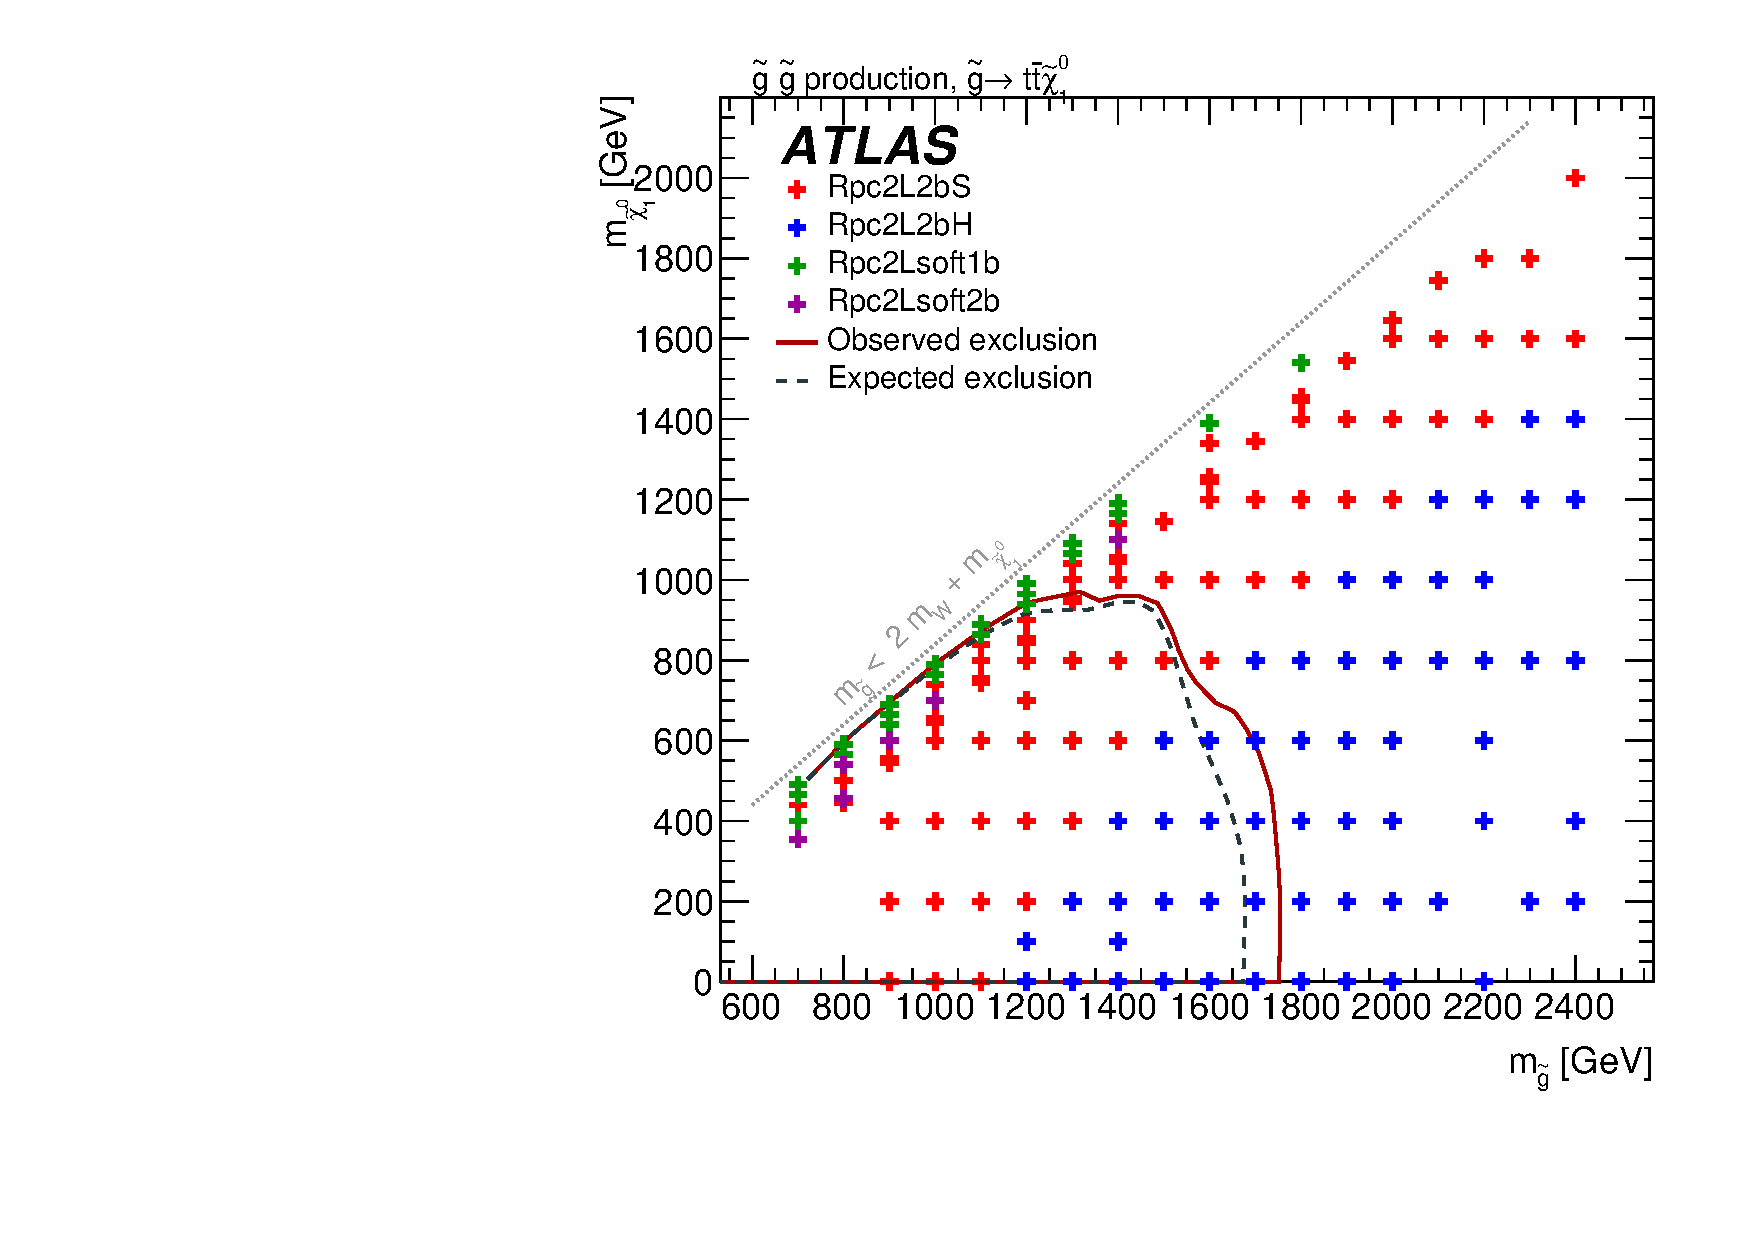
\includegraphics[width=\textwidth]{best_Rpc2L2b}\caption{}\label{fig:best_Rpc2L2b}\end{subfigure}
\begin{subfigure}[t]{0.49\textwidth}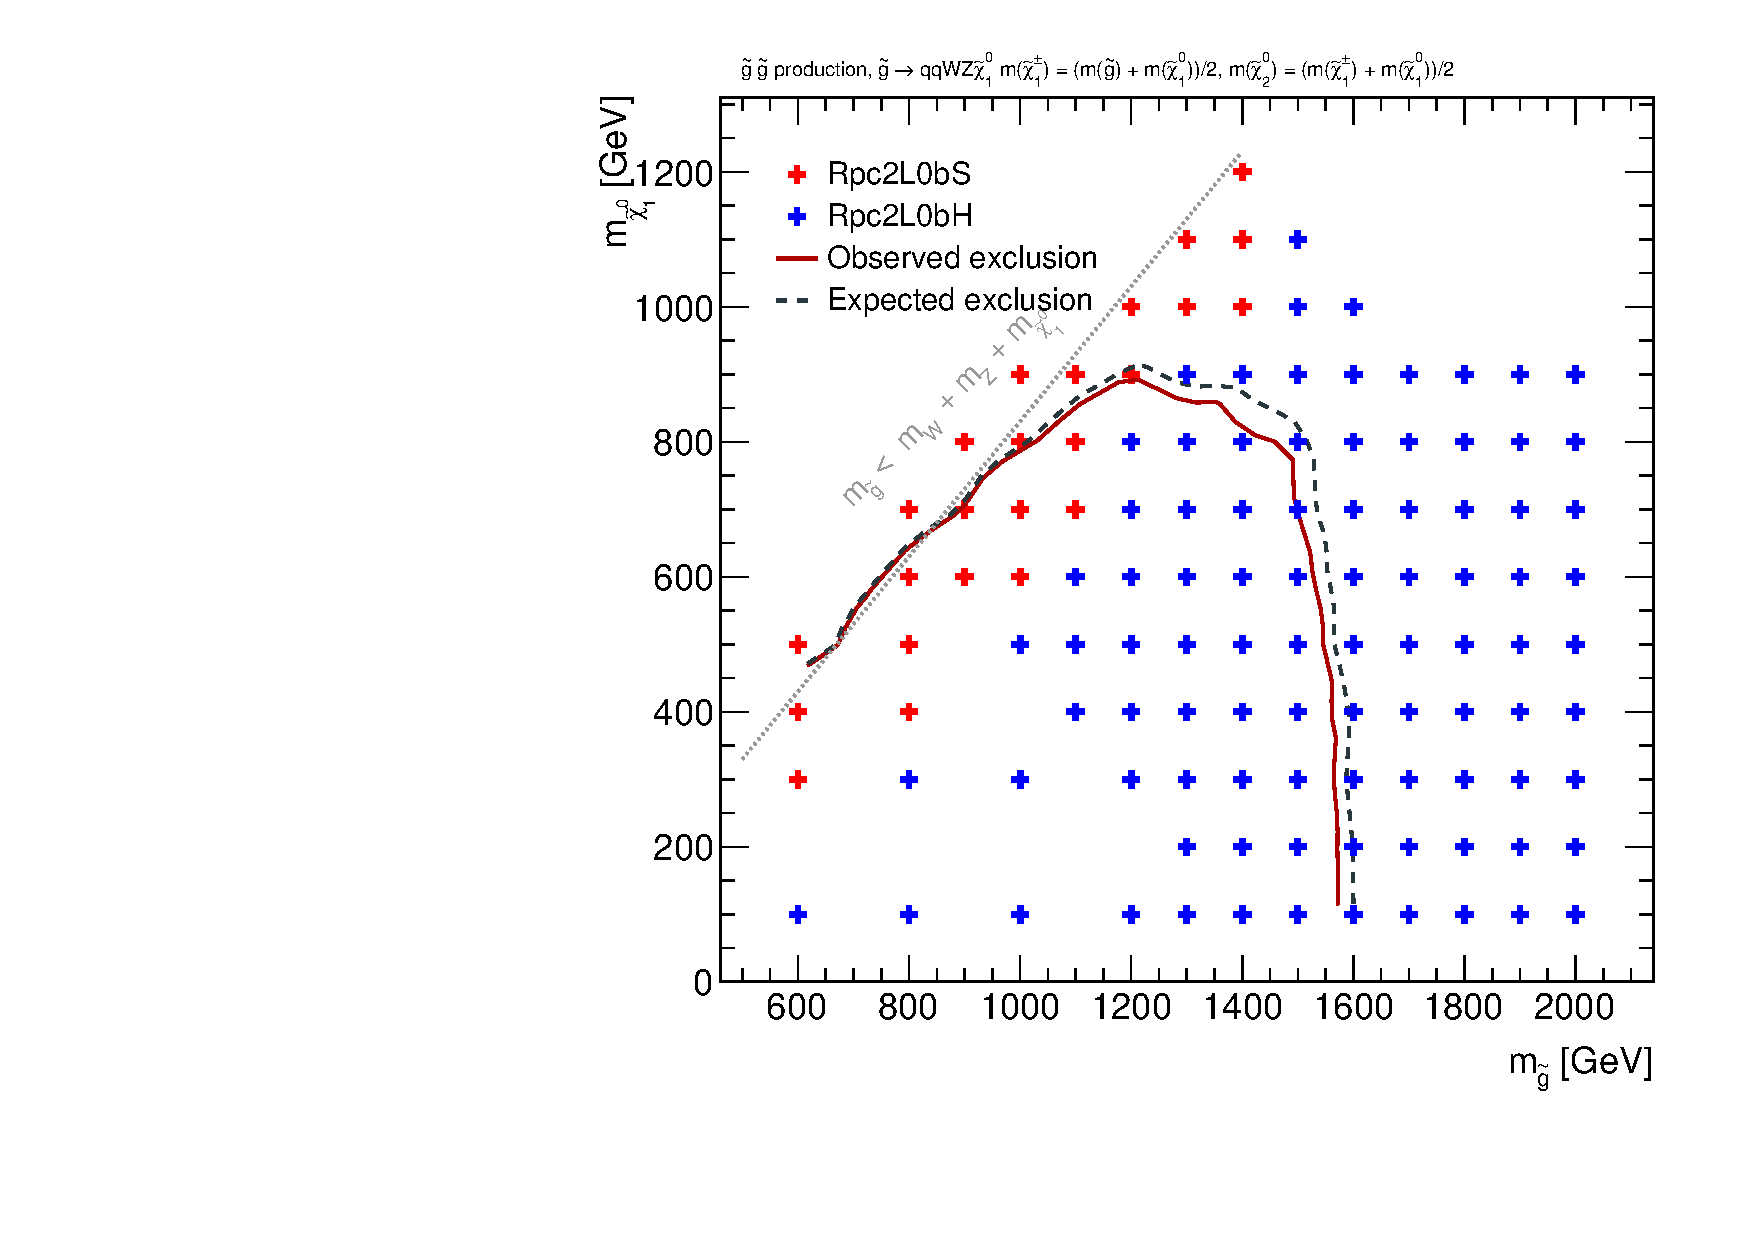
\includegraphics[width=\textwidth]{best_Rpc2L0b}\caption{}\label{fig:best_Rpc2L0b}\end{subfigure}
\caption{Illustration of the best expected signal region per signal grid point for the (a)  
$\gluino\to q\bar q (\ell\ell/\nu\nu)\tilde\chi^0_1$ and (b) $\gluino\to q\bar q' WZ\tilde\chi^0_1$ models. 
This mapping is used for the final combined exclusion limits.}
\label{fig:best_SR1}
\end{figure}

\begin{figure}[htb!]
\centering
\begin{subfigure}[t]{0.49\textwidth}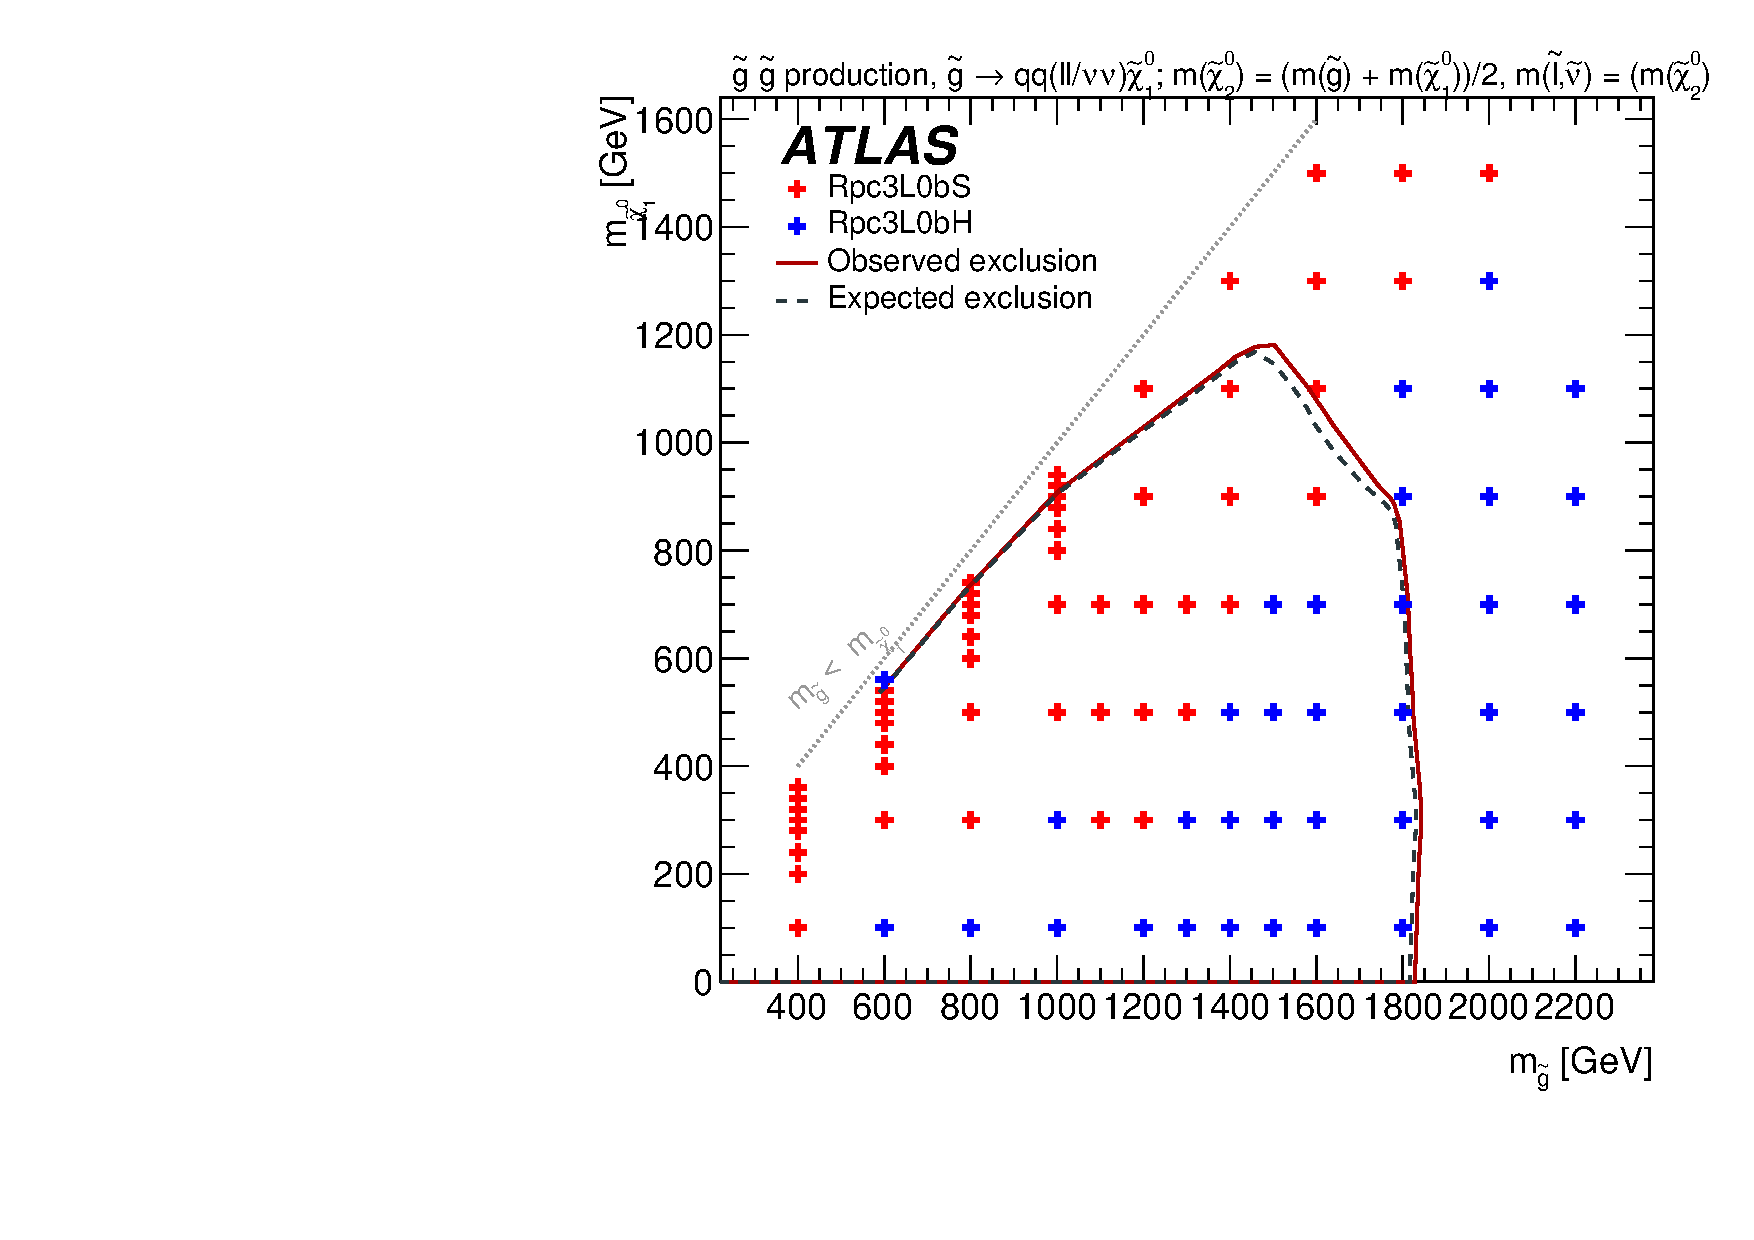
\includegraphics[width=\textwidth]{best_Rpc3L0b}\caption{}\label{fig:best_Rpc3L0b}\end{subfigure}
\begin{subfigure}[t]{0.49\textwidth}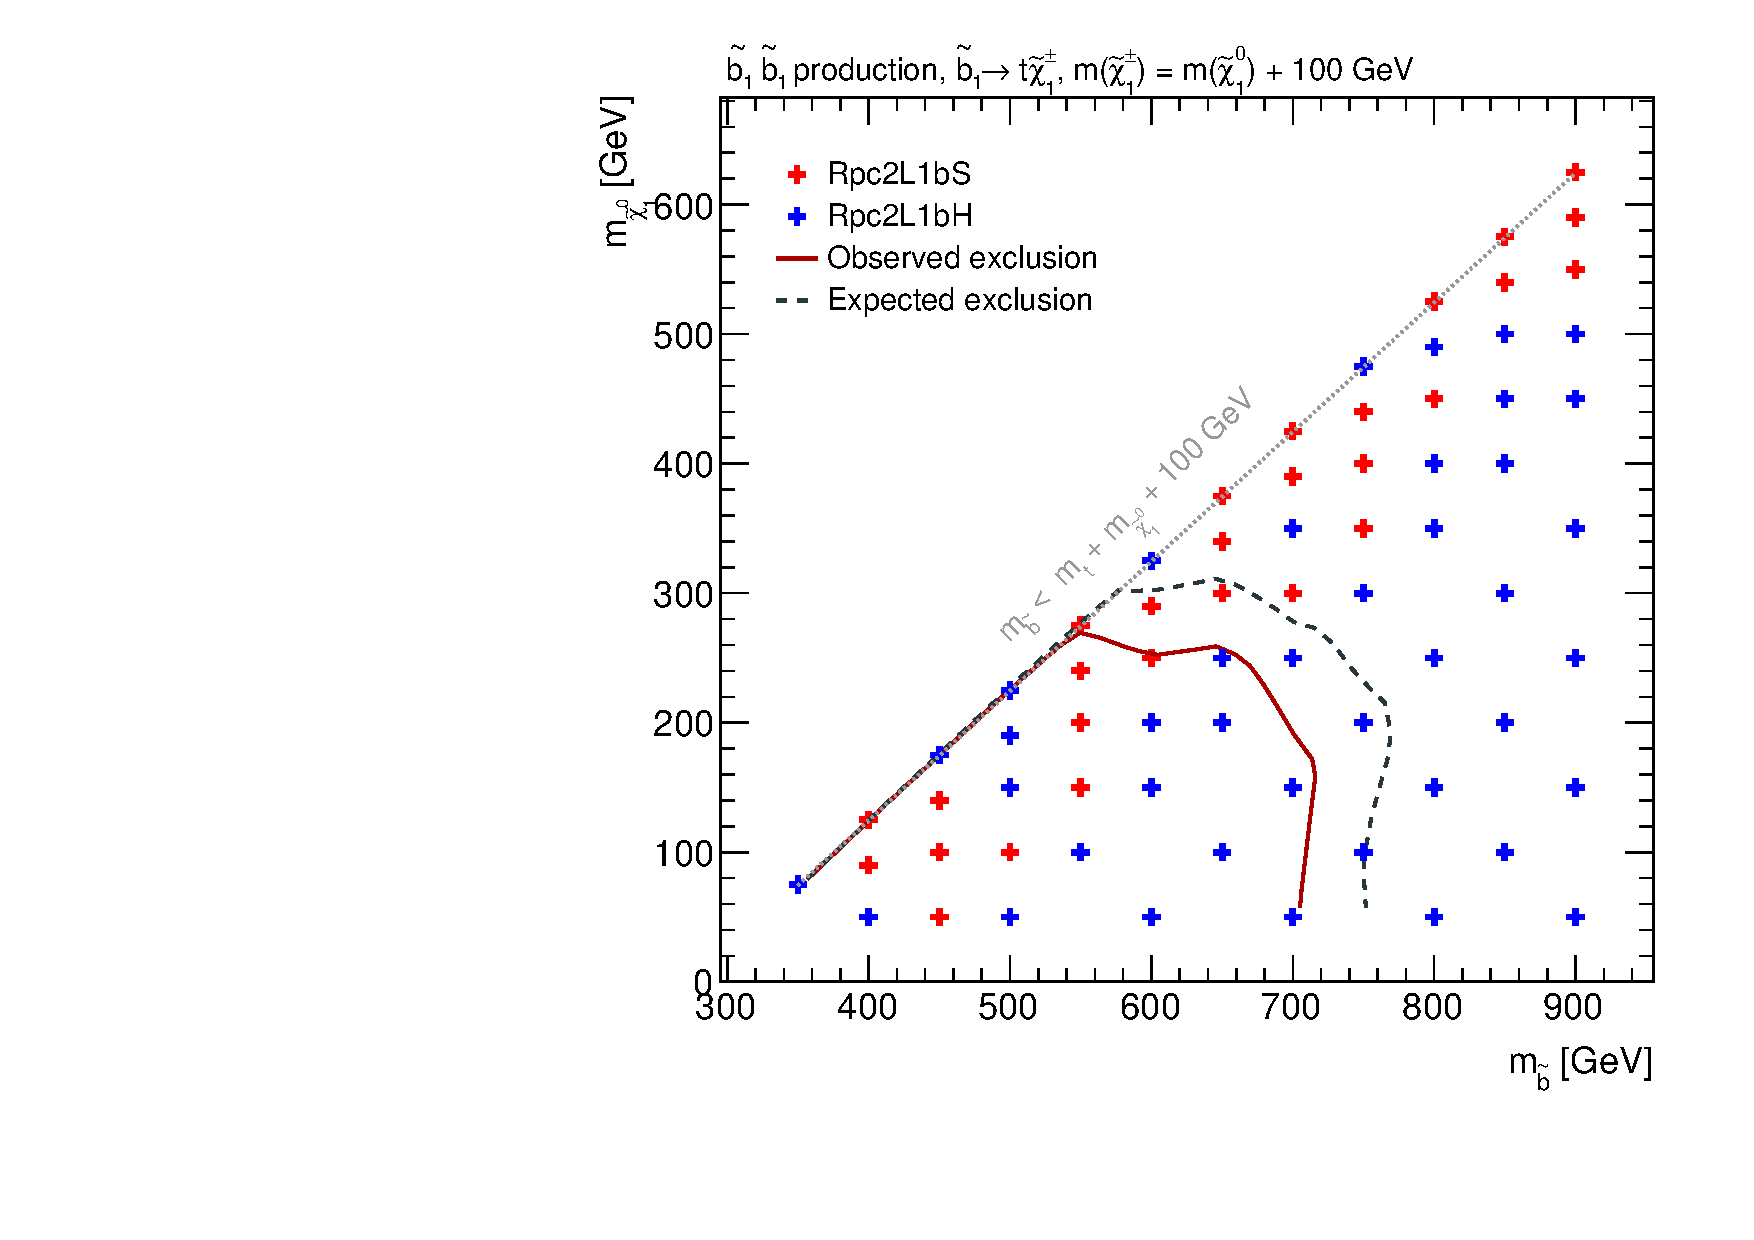
\includegraphics[width=\textwidth]{best_Rpc2L1b}\caption{}\label{fig:best_Rpc2L1b}\end{subfigure}
\caption{Illustration of the best expected signal region per signal grid point for the 
(a) $\gluino\to q\bar q' \ell/\nu \ell/\nu \tilde\chi^0_1$ and (b) $\sbottom\to t W \tilde\chi^0_1$ models. 
This mapping is used for the final combined exclusion limits.}
\label{fig:best_SR2}
\end{figure}

\newpage

\section{Upper limit on cross section}
\label{app:aux.ULcs}

\begin{figure}[htb!]
\centering
\begin{subfigure}[t]{0.49\textwidth}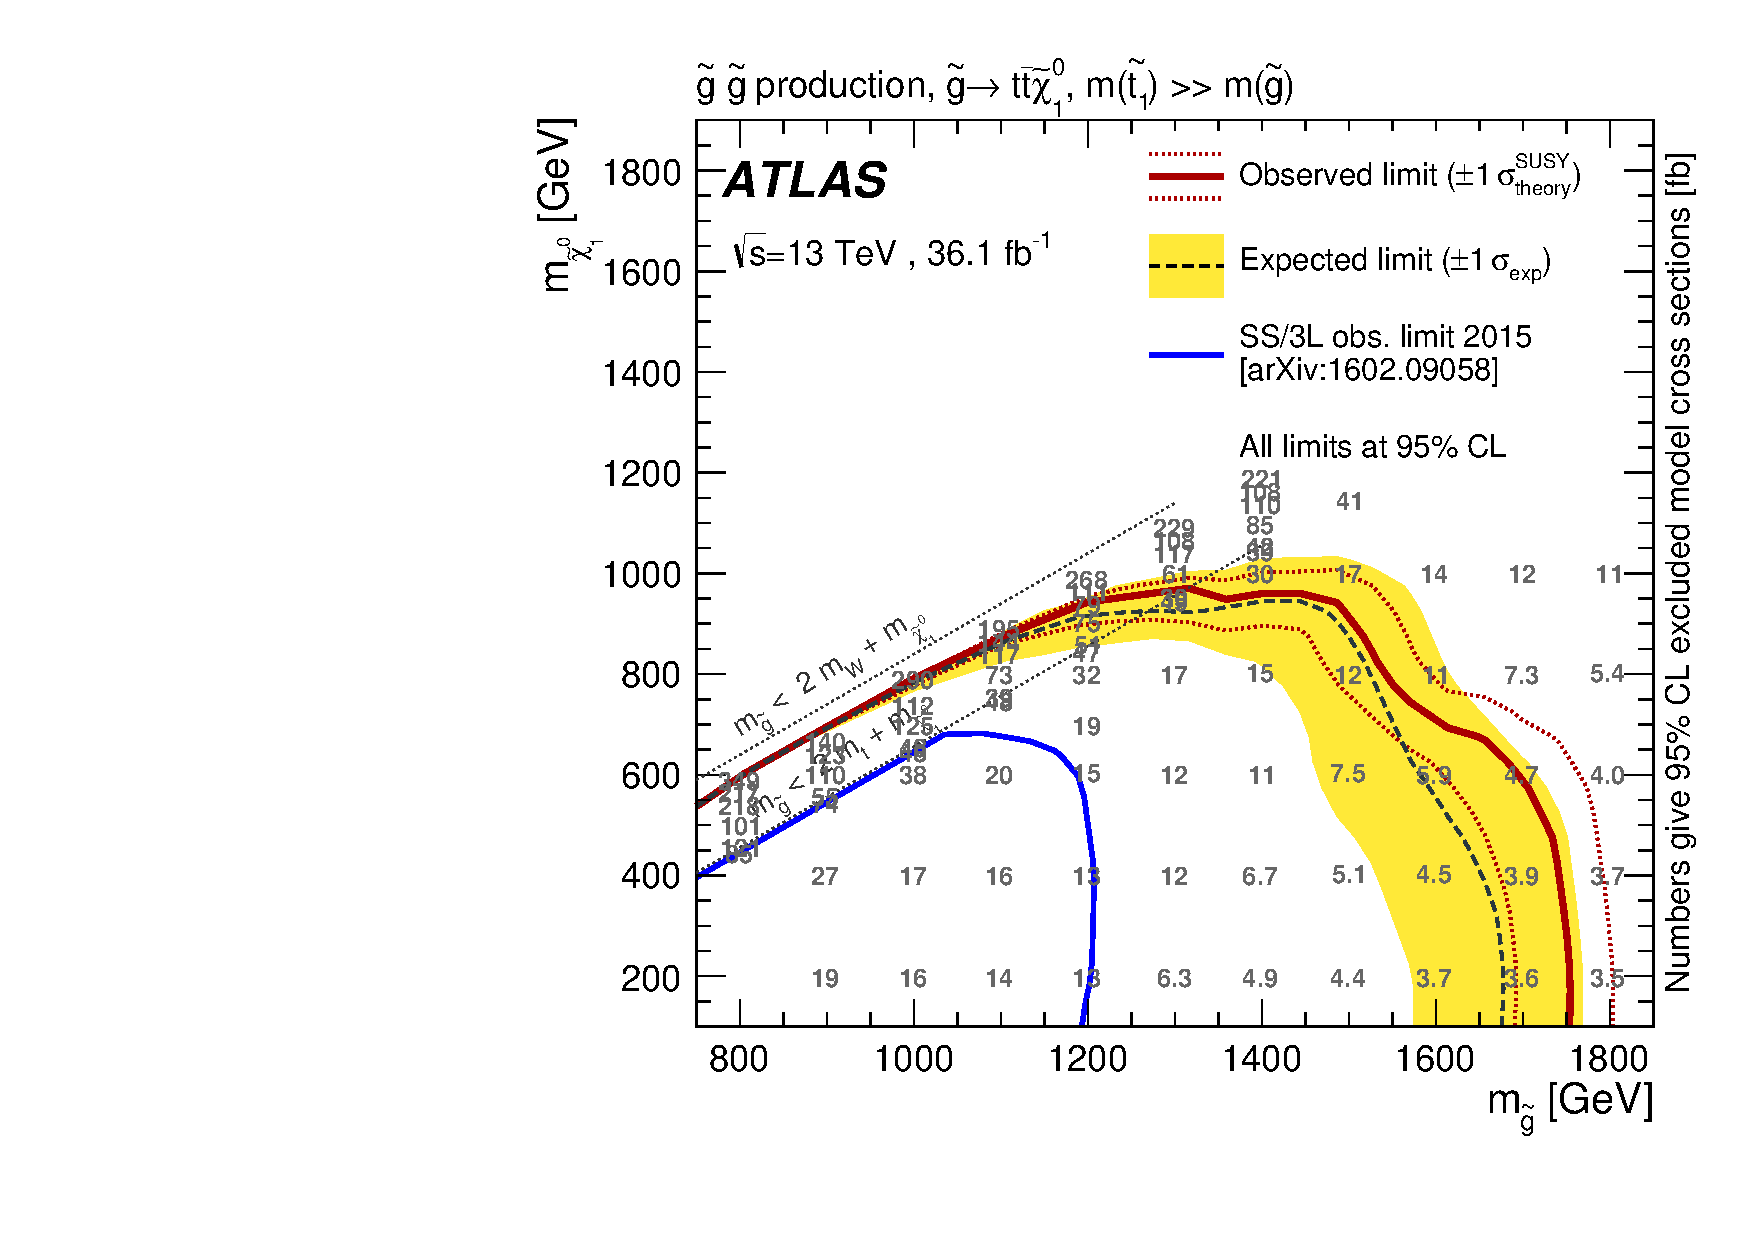
\includegraphics[width=\textwidth]{GreyNumbers/Gtt_SRbest}\caption{Rpc2L2bS/H, Rpc2Lsoft1b/2b}\label{fig:GN_limits_feynman_gtt}\end{subfigure}
\begin{subfigure}[t]{0.49\textwidth}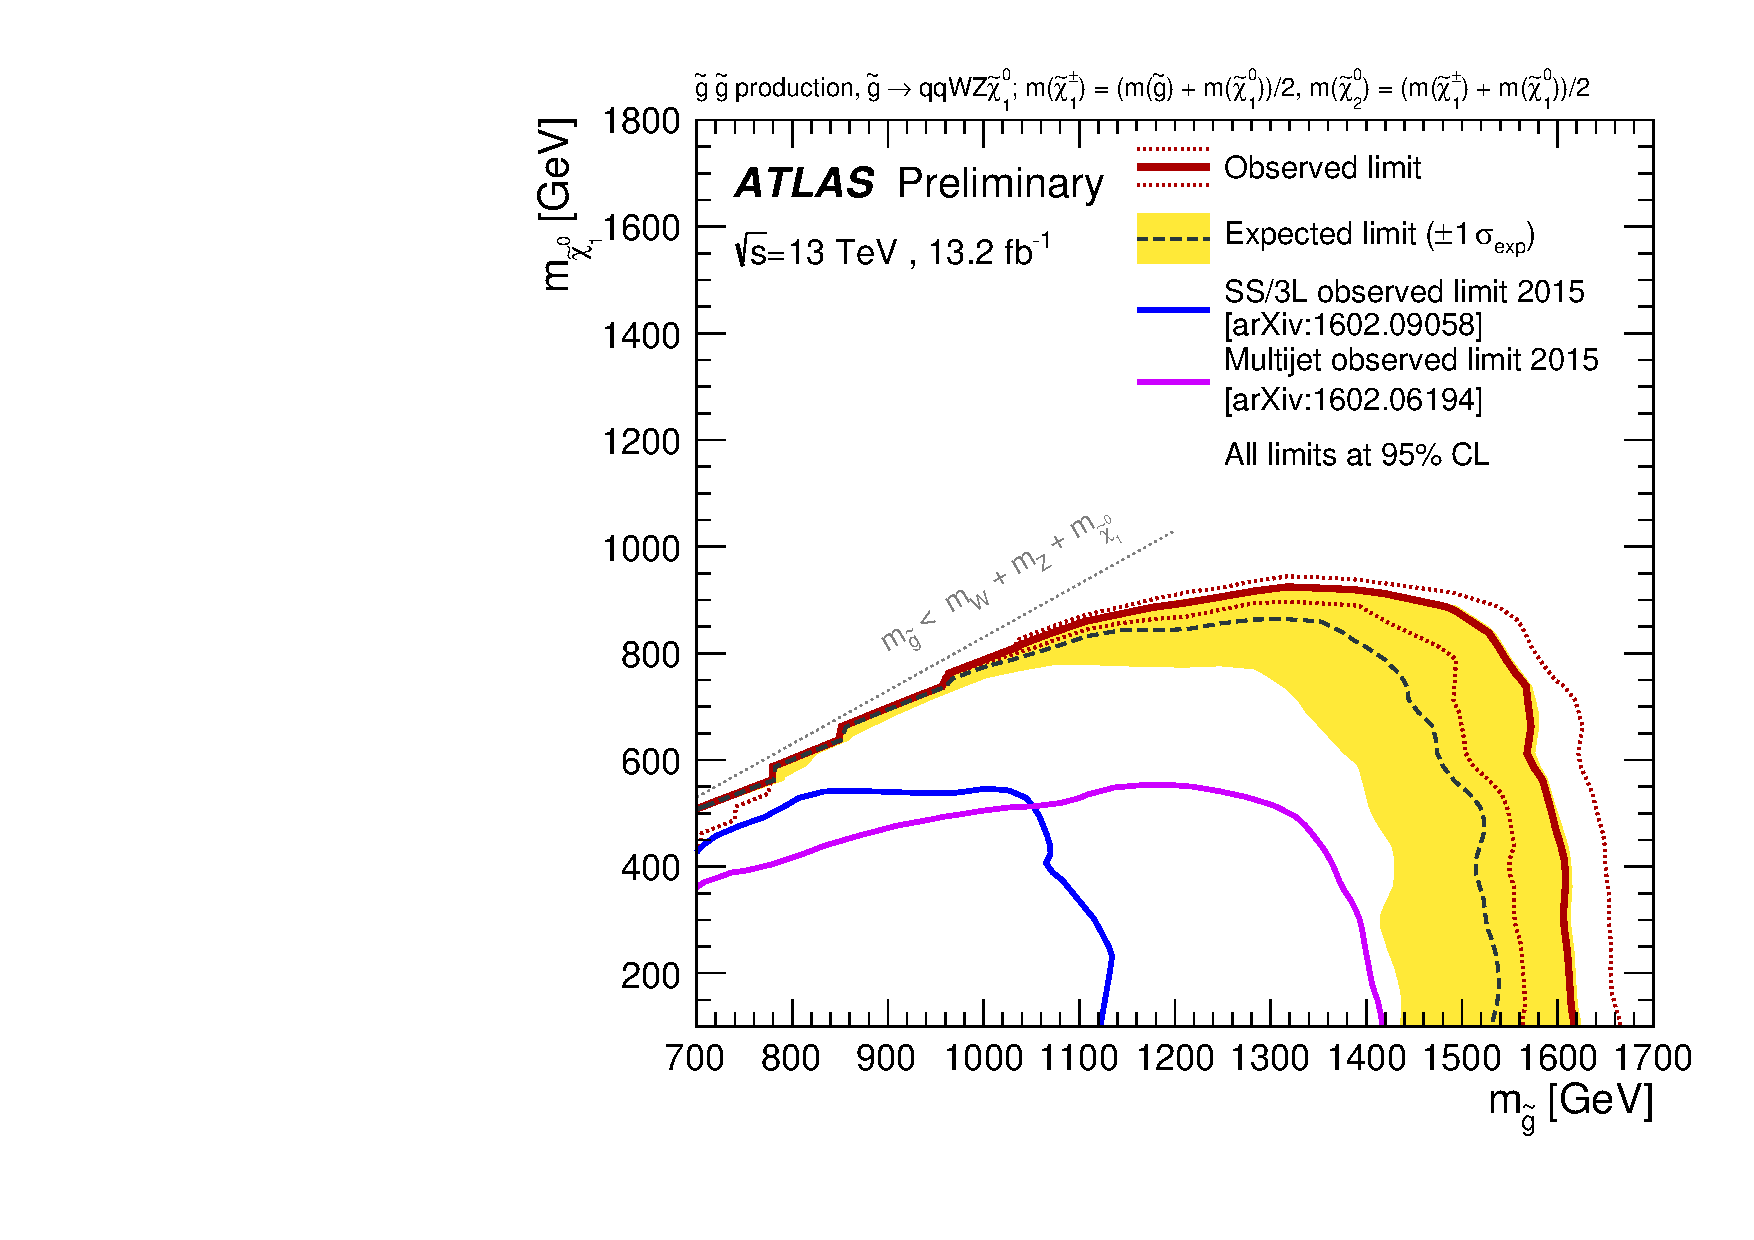
\includegraphics[width=\textwidth]{GreyNumbers/2stepWZ_SRbest}\caption{Rpc2L0bS, Rpc2L0bH}\label{fig:GN_limits_feynman_gg2WZ}\end{subfigure}

\caption{Observed and expected exclusion limits on the $\tilde{g}$ and \ninoone masses 
in the context of RPC SUSY scenarios with simplified mass spectra. The signal regions used to obtain the limits are specified in the subtitle of each scenario. All limits are computed at 95\% CL. 
%Figures~\ref{fig:GN_limits_feynman_gtt}--\ref{fig:GN_limits_feynman_b1b1}, the grey diagonal lines indicate the kinematic limit for the decays in each 
%specified scenario and results are compared with the observed limits obtained by previous ATLAS searches~\cite{paperSS3L,Aad:2016jxj}. 
The grey numbers show 95\% CL upper limits on production cross-sections (in fb) obtained using the signal efficiency and acceptance specific to each model.}
\label{fig:Results_Limits_RPC_GN} 
\end{figure} 

\begin{figure}[htb!]
\centering
\begin{subfigure}[t]{0.49\textwidth}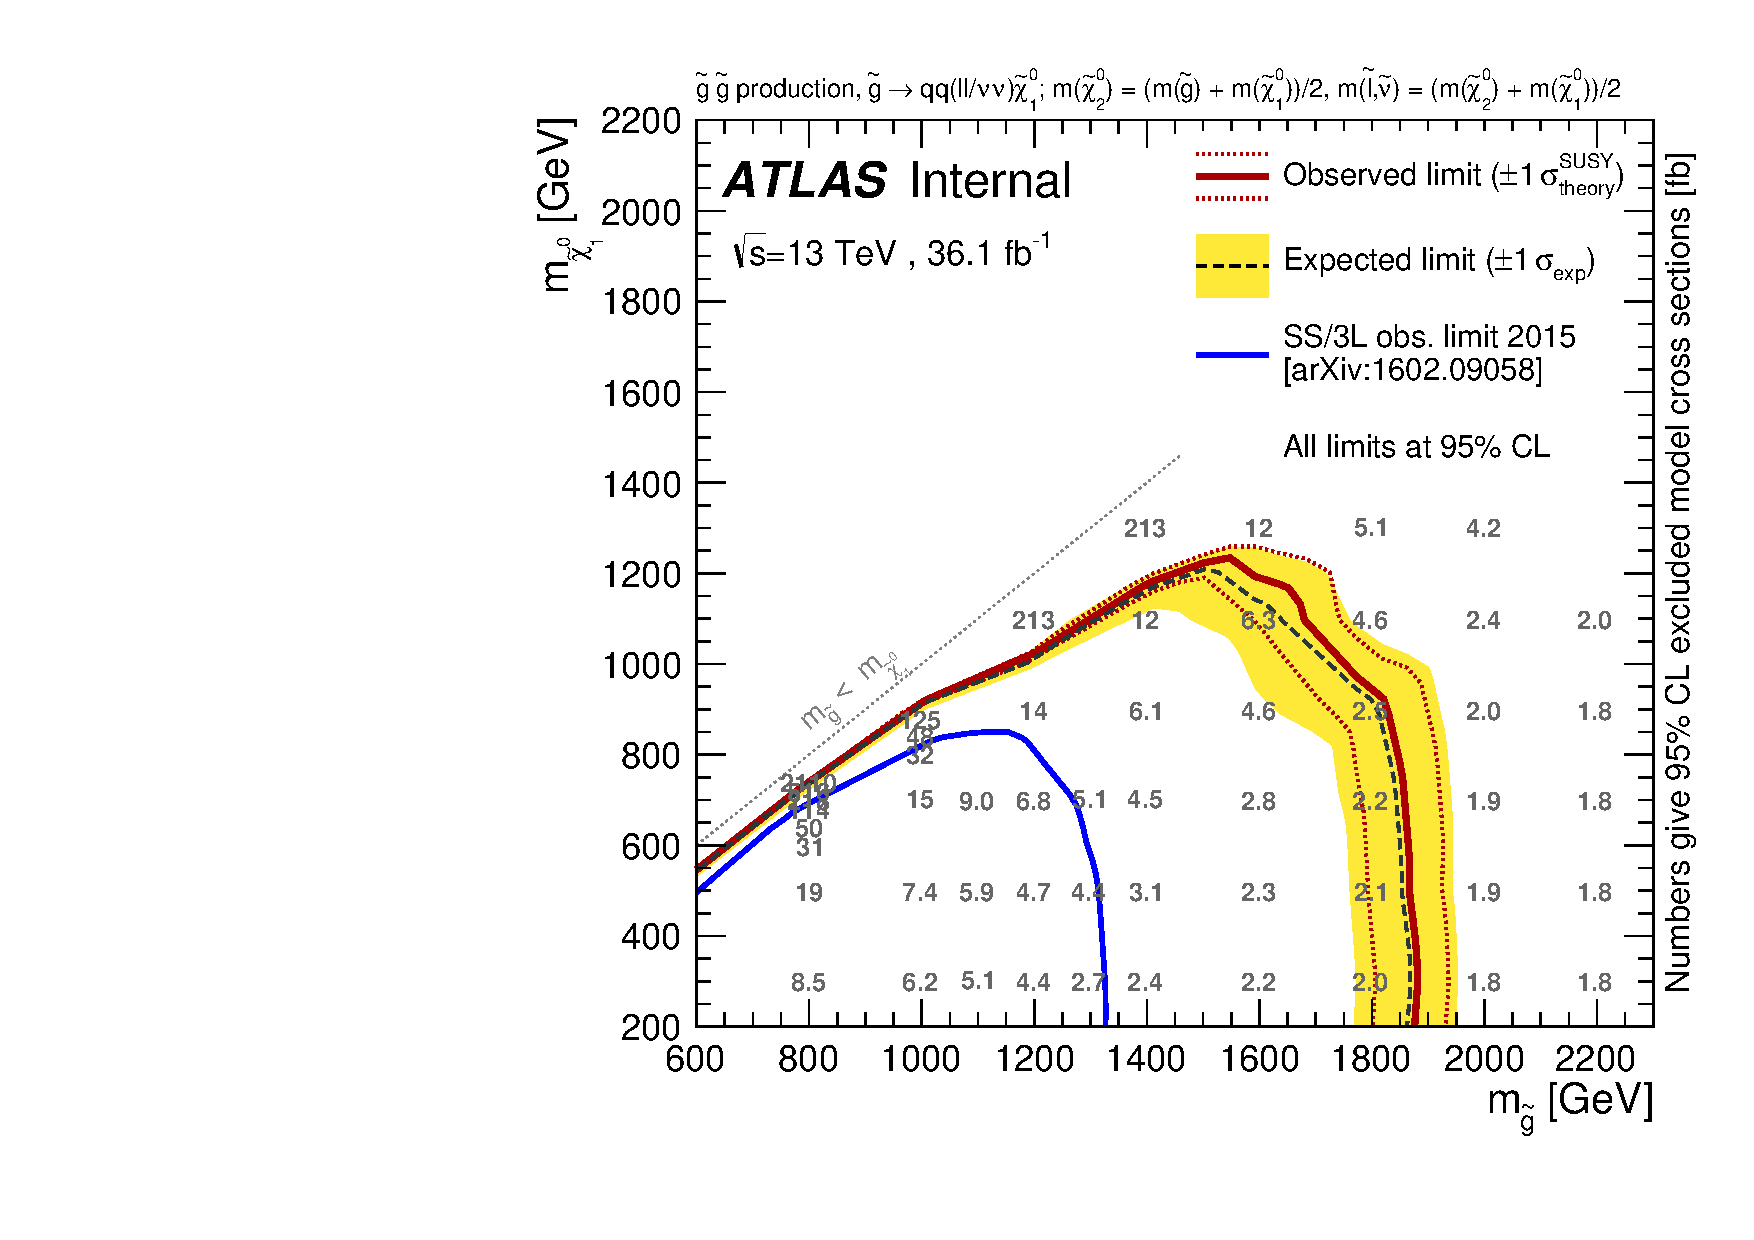
\includegraphics[width=\textwidth]{GreyNumbers/GSL_SRbest.pdf}\caption{Rpc3L0bS, Rpc3L0bH}\label{fig:GN_limits_feynman_gg2sl}\end{subfigure}
\begin{subfigure}[t]{0.49\textwidth}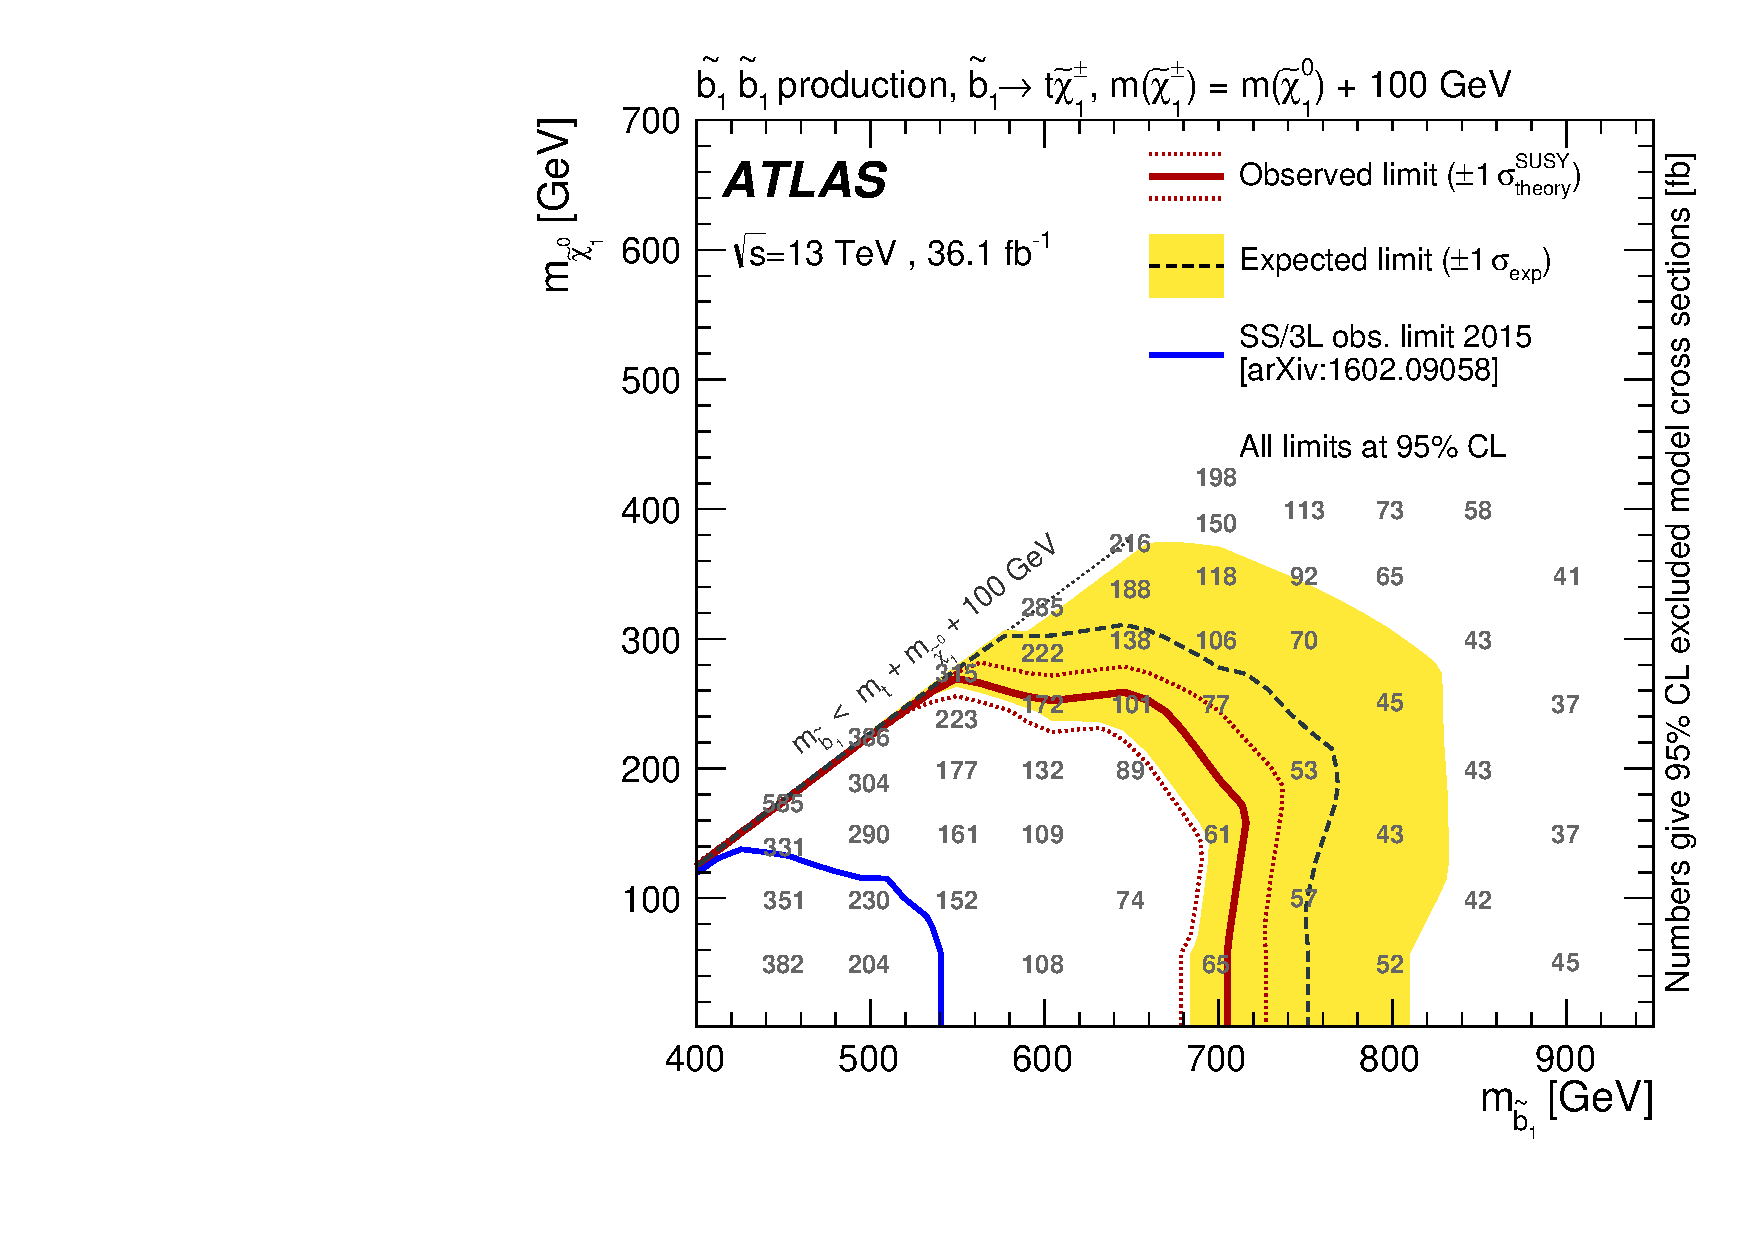
\includegraphics[width=\textwidth]{GreyNumbers/Btt_SRbest.pdf}\caption{Rpc2L1bS, Rpc2L1bH}\label{fig:GN_limits_feynman_b1b1}\end{subfigure}

\caption{Observed and expected exclusion limits on the $\tilde{g}$, \sbottomone, and \ninoone masses 
in the context of RPC SUSY scenarios with simplified mass spectra. The signal regions used to obtain the limits are specified in the subtitle of each scenario. All limits are computed at 95\% CL. 
%Figures~\ref{fig:GN_limits_feynman_gtt}--\ref{fig:GN_limits_feynman_b1b1}, the grey diagonal lines indicate the kinematic limit for the decays in each 
%specified scenario and results are compared with the observed limits obtained by previous ATLAS searches~\cite{paperSS3L,Aad:2016jxj}. 
The grey numbers show 95\% CL upper limits on production cross-sections (in fb) obtained using the signal efficiency and acceptance specific to each model.}
\label{fig:Results_Limits_RPC_GN} 
\end{figure} 


\section{Signal region cutflow}
\label{app:aux.SRcut}

\begin{table}[htb!]\centering\def\arraystretch{1.2}\begin{tabular}{|l|c|}\hline
   \multicolumn{2}{|l|}{Rpc2L2bS,\quad$\gluino\gluino$ production,\quad$\gluino\to \ttbar\ninoone$}\\
   \multicolumn{2}{|l|}{$m_{\gluino}= 1.5 \TeV$, $m_{\ninoone}= 800 \GeV$}\\\hline
   MC events generated  & 98000 \\\hline
   Expected for 36.1 \ifb  & $5.1\times 10^2$ \\
   $\geq 2$ SS leptons ($\pt>20 \GeV$)  & $19.96 \pm 0.35$ \\
   Trigger  & $19.17 \pm 0.35$ \\
   $\ge 2$ $b$-jets ($\pt>20 \GeV$)  & $16.10 \pm 0.32$ \\
   $\ge 6$ jets ($\pt>25 \GeV$)  & $13.11 \pm 0.28$ \\
   $\met>200 \GeV$  & $10.17 \pm 0.26$ \\
   $\meff>0.6 \TeV$  & $10.17 \pm 0.26$ \\
   $\met>0.25\times\meff$  & $5.94 \pm 0.20$ \\
\hline\end{tabular}
\caption{Number of signal events at different stages of the Rpc2L2bS signal region selection. 
Only statistical uncertainties are shown.}
\end{table}

\begin{table}[htb!]\centering\def\arraystretch{1.2}\begin{tabular}{|l|c|}\hline
   \multicolumn{2}{|l|}{Rpc2L2bH,\quad$\gluino\gluino$ production,\quad$\gluino\to \ttbar\ninoone$}\\
   \multicolumn{2}{|l|}{$m_{\gluino}=1.7 \TeV$, $m_{\ninoone}=200 \GeV$}\\\hline
   MC events generated  & 98000 \\\hline
   Expected for 36.1 \ifb  & $1.7\times 10^2$ \\
   $\geq 2$ SS leptons ($\pt>20 \GeV$)  & $7.32 \pm 0.13$ \\
   Trigger  & $7.19 \pm 0.13$ \\
   $\ge 2$ $b$-jets ($\pt>20 \GeV$)  & $5.81 \pm 0.11$ \\
   $\ge 6$ jets ($\pt>40 \GeV$)  & $4.92 \pm 0.11$ \\
   $\meff>1.8 \TeV$  & $3.93 \pm 0.09$ \\
   $\met>0.15\times\meff$  & $3.12 \pm 0.08$ \\
\hline\end{tabular}
\caption{Number of signal events at different stages of the Rpc2L2bH signal region selection. 
Only statistical uncertainties are shown.}\end{table}

\begin{table}[htb!]\centering\def\arraystretch{1.2}\begin{tabular}{|l|c|}\hline
   \multicolumn{2}{|l|}{Rpc2Lsoft1b,\quad$\gluino\gluino$ production,\quad$\gluino\to tWb\ninoone$}\\
   \multicolumn{2}{|l|}{$m_{\gluino}=1.2 \TeV$, $m_{\ninoone}=940 \GeV$}\\\hline
   MC events generated  & 50000 \\\hline
   Expected for 36.1 \ifb  & $3.1\times 10^3$ \\
   $\geq 2$ SS leptons ($100>\pt>20,10$~GeV)  & $101.9 \pm 2.7$ \\
   Trigger  & $89.3 \pm 2.5$ \\
   $\ge 1$ $b$-jet ($\pt>20 \GeV$)  & $75.1 \pm 2.3$ \\
   $\ge 6$ jets ($\pt>25 \GeV$)  & $31.5 \pm 1.5$ \\
   $\met>100 \GeV$  & $23.0 \pm 1.3$ \\
   $\met>0.3\times\meff$  & $6.5 \pm 0.7$ \\
\hline\end{tabular}
\caption{Number of signal events at different stages of the Rpc2Lsoft1b signal region selection. 
Only statistical uncertainties are shown.}\end{table}

\begin{table}[htb!]\centering\def\arraystretch{1.2}\begin{tabular}{|l|c|}\hline
   \multicolumn{2}{|l|}{Rpc2Lsoft2b,\quad$\gluino\gluino$ production,\quad$\gluino\to tWb\ninoone$}\\
   \multicolumn{2}{|l|}{$m_{\gluino}=1.2 \TeV$, $m_{\ninoone}=900 \GeV$}\\\hline
   MC events generated  & 50000 \\\hline
   Expected for 36.1 \ifb  & $3.1\times 10^3$ \\
   $\geq 2$ SS leptons ($100>\pt>20,10$~GeV)  & $91.8 \pm 2.6$ \\
   Trigger  & $79.7 \pm 2.4$ \\
   $\ge 2$ $b$-jets ($\pt>20 \GeV$)  & $41.3 \pm 1.7$ \\
   $\ge 6$ jets ($\pt>25 \GeV$)  & $21.4 \pm 1.2$ \\
   $\met>200 \GeV$  & $8.7 \pm 0.7$ \\
   $\meff>0.6 \TeV$  & $8.7 \pm 0.7$ \\
   $\met>0.25\times\meff$  & $6.7 \pm 0.6$ \\
\hline\end{tabular}
\caption{Number of signal events at different stages of the Rpc2Lsoft2b signal region selection. 
Only statistical uncertainties are shown.}\end{table}

\begin{table}[htb!]\centering\def\arraystretch{1.2}\begin{tabular}{|l|c|}\hline
   \multicolumn{2}{|l|}{Rpc2L0bS,\quad$\gluino\gluino$ production,\quad$\gluino\to q\bar q^{'}WZ\ninoone$}\\
   \multicolumn{2}{|l|}{$m_{\gluino}=1.2 \TeV$, $(m_{\chargino} - 150) = (m_{\tilde\chi_2^0} - 75) = m_{\ninoone}=900 \GeV$}\\\hline
   MC events generated  & 19000 \\\hline
   Expected for 36.1 \ifb  & $3.1\times 10^3$ \\
   $\geq 2$ SS leptons ($\pt>20 \GeV$)  & $64 \pm 4$ \\
   Trigger  & $58.6 \pm 3.3$ \\
   no $b$-jet ($\pt>20 \GeV$)  & $46.3 \pm 3.0$ \\
   $\ge 6$ jets ($\pt>25 \GeV$)  & $26.6 \pm 2.4$ \\
   $\met>150 \GeV$  & $16.3 \pm 2.0$ \\
   $\met>0.25\times\meff$  & $9.0 \pm 1.3$ \\
\hline\end{tabular}
\caption{Number of signal events at different stages of the Rpc2L0bS signal region selection. 
Only statistical uncertainties are shown.}\end{table}

\begin{table}[htb!]\centering\def\arraystretch{1.2}\begin{tabular}{|l|c|}\hline
   \multicolumn{2}{|l|}{Rpc2L0bH,\quad$\gluino\gluino$ production,\quad$\gluino\to q\bar q^{'}WZ\ninoone$}\\
   \multicolumn{2}{|l|}{$m_{\gluino}=1.6 \TeV$, $(m_{\chargino} - 750) = (m_{\tilde\chi_2^0} - 375) = m_{\ninoone}=100 \GeV$}\\\hline
   MC events generated  & 20000 \\\hline
   Expected for 36.1 \ifb  & $2.9\times 10^2$ \\
   $\geq 2$ SS leptons ($\pt>20 \GeV$)  & $12.8 \pm 0.5$ \\
   Trigger  & $12.5 \pm 0.5$ \\
   no $b$-jet ($\pt>20 \GeV$)  & $8.5 \pm 0.4$ \\
   $\ge 6$ jets ($\pt>40 \GeV$)  & $7.12 \pm 0.35$ \\
   $\met>250 \GeV$  & $5.13 \pm 0.29$ \\
   $\meff>0.9 \TeV$  & $5.13 \pm 0.29$ \\
\hline\end{tabular}
\caption{Number of signal events at different stages of the Rpc2L0bH signal region selection. 
Only statistical uncertainties are shown.}\end{table}

\begin{table}[htb!]\centering\def\arraystretch{1.2}\begin{tabular}{|l|c|}\hline
   \multicolumn{2}{|l|}{Rpc3L0bS,\quad$\gluino\gluino$ production,\quad$\gluino\to q\bar q(\tilde\ell\ell/\tilde\nu\nu)$}\\
   \multicolumn{2}{|l|}{$m_{\gluino}=1.4 \TeV$, $(m_{\tilde\chi_2^0} - 150) = (m_{\tilde\ell, \tilde\nu} - 75) = m_{\ninoone}=1100 \GeV$}\\\hline
   MC events generated  & 20000 \\\hline
   Expected for 36.1 \ifb  & $9.1\times 10^2$ \\
   $\geq 3$ leptons ($\pt>20,20,10$~GeV)  & $76.9 \pm 2.1$ \\
   Trigger  & $76.0 \pm 2.0$ \\
   no $b$-jet ($\pt>20 \GeV$)  & $67.5 \pm 1.9$ \\
   $\ge 4$ jets ($\pt>40 \GeV$)  & $31.6 \pm 1.3$ \\
   $\met>200 \GeV$  & $17.1 \pm 1.0$ \\
   $\meff>0.6 \TeV$  & $17.1 \pm 1.0$ \\
\hline\end{tabular}
\caption{Number of signal events at different stages of the Rpc3L0bS signal region selection. 
Only statistical uncertainties are shown.}\end{table}

\begin{table}[htb!]\centering\def\arraystretch{1.2}\begin{tabular}{|l|c|}\hline
   \multicolumn{2}{|l|}{Rpc3L0bH,\quad$\gluino\gluino$ production,\quad$\gluino\to q\bar q(\tilde\ell\ell/\tilde\nu\nu)$}\\
   \multicolumn{2}{|l|}{$m_{\gluino}=1.8 \TeV$, $(m_{\tilde\chi_2^0} - 850) = (m_{\tilde\ell, \tilde\nu} - 375) = m_{\ninoone}=100 \GeV$}\\\hline
   MC events generated  & 20000 \\\hline
   Expected for 36.1 \ifb  & $1.0\times 10^{2}$ \\
   $\geq 3$ leptons ($\pt>20,20,10$~GeV)  & $9.98 \pm 0.25$ \\
   Trigger  & $9.94 \pm 0.25$ \\
   no $b$-jet ($\pt>20 \GeV$)  & $8.44 \pm 0.23$ \\
   $\ge 4$ jets ($\pt>40 \GeV$)  & $7.79 \pm 0.22$ \\
   $\met>200 \GeV$  & $6.58 \pm 0.21$ \\
   $\meff>1.6 \TeV$  & $6.56 \pm 0.21$ \\
\hline\end{tabular}
\caption{Number of signal events at different stages of the Rpc3L0bH signal region selection. 
Only statistical uncertainties are shown.}\end{table}

\begin{table}[htb!]\centering\def\arraystretch{1.2}\begin{tabular}{|l|c|}\hline
   \multicolumn{2}{|l|}{Rpc2L1bS,\quad$\sbottomone\sbottomonebar$ production,\quad$\sbottomone\to t\tilde\chi_1^{-}\to t W^-
\ninoone$}\\
   \multicolumn{2}{|l|}{$m_{\sbottomone}=600 \GeV$, $m_{\chargino} = 350 \GeV$, $m_{\ninoone}=250 \GeV$}\\\hline
   MC events generated  & 10000 \\\hline
   Expected for 36.1 \ifb  & $6.3\times 10^3$ \\
   $\geq 2$ SS leptons ($\pt>20 \GeV$)  & $221 \pm 4$ \\
   Trigger  & $201 \pm 4$ \\
   $\ge 1$ $b$-jet ($\pt>20 \GeV$)  & $173 \pm 4$ \\
   $\ge 6$ jets ($\pt>25 \GeV$)  & $66.3 \pm 2.2$ \\
   $\met>150 \GeV$  & $36.5 \pm 1.7$ \\
   $\meff>0.6 \TeV$  & $36.1 \pm 1.7$ \\
   $\met>0.25\times\meff$  & $15.1 \pm 1.1$ \\
\hline\end{tabular}
\caption{Number of signal events at different stages of the Rpc2L1bS signal region selection. 
Only statistical uncertainties are shown.}\end{table}

\begin{table}[htb!]\centering\def\arraystretch{1.2}\begin{tabular}{|l|c|}\hline
   \multicolumn{2}{|l|}{Rpc2L1bH,\quad$\sbottomone\sbottomonebar$ production,\quad$\sbottomone\to t\tilde\chi_1^{-}$}\\
   \multicolumn{2}{|l|}{$m_{\sbottomone}=750 \GeV$, $m_{\chargino} = 200 \GeV$, $m_{\ninoone}=100 \GeV$}\\\hline
   MC events generated  & 10000 \\\hline
   Expected for 36.1 \ifb  & $1.6\times 10^3$ \\
   $\geq 2$ SS leptons ($\pt>20 \GeV$)  & $71.1 \pm 1.2$ \\
   Trigger  & $66.4 \pm 1.2$ \\
   $\ge 1$ $b$-jet ($\pt>20 \GeV$)  & $56.6 \pm 1.1$ \\
   $\ge 6$ jets ($\pt>25 \GeV$)  & $27.7 \pm 0.7$ \\
   $\met>250 \GeV$  & $12.5 \pm 0.5$ \\
   $\met>0.2\times\meff$  & $9.5 \pm 0.4$ \\
\hline\end{tabular}
\caption{Number of signal events at different stages of the Rpc2L1bH signal region selection. 
Only statistical uncertainties are shown.}\end{table}

\begin{table}[htb!]\centering\def\arraystretch{1.2}\begin{tabular}{|l|c|}\hline
   \multicolumn{2}{|l|}{Rpc3LSS1b,\quad$\stopone\stoponebar$ production,\quad$\stopone\to t\ninotwo\to \tilde t W^\pm \chi_1^\mp$}\\
   \multicolumn{2}{|l|}{$m_{\stopone}=700 \GeV$, $m_{\ninotwo}=525 \GeV$, $m_{\chargino}\approx m_{\ninoone}=425 \GeV$}\\\hline
   MC events generated  & 5000 \\\hline
   Expected for 36.1 \ifb  & $2.4\times 10^3$ \\
   $\geq 3$ SS leptons ($\pt>20,20,10$~GeV), $Z\to e^\pm e^\pm$ veto  & $4.6 \pm 0.5$ \\
   Trigger  & $4.5 \pm 0.5$ \\
   $\ge 1$ $b$-jet ($\pt>20 \GeV$)  & $3.6 \pm 0.4$ \\
\hline\end{tabular}
\caption{Number of signal events at different stages of the Rpc3LSS1b signal region selection. 
Only statistical uncertainties are shown.}\end{table}

\section{Acceptance and Efficiency}
\label{app:aux.AccEff}
\begin{figure}[htb!]
\centering
\begin{subfigure}[t]{0.49\textwidth}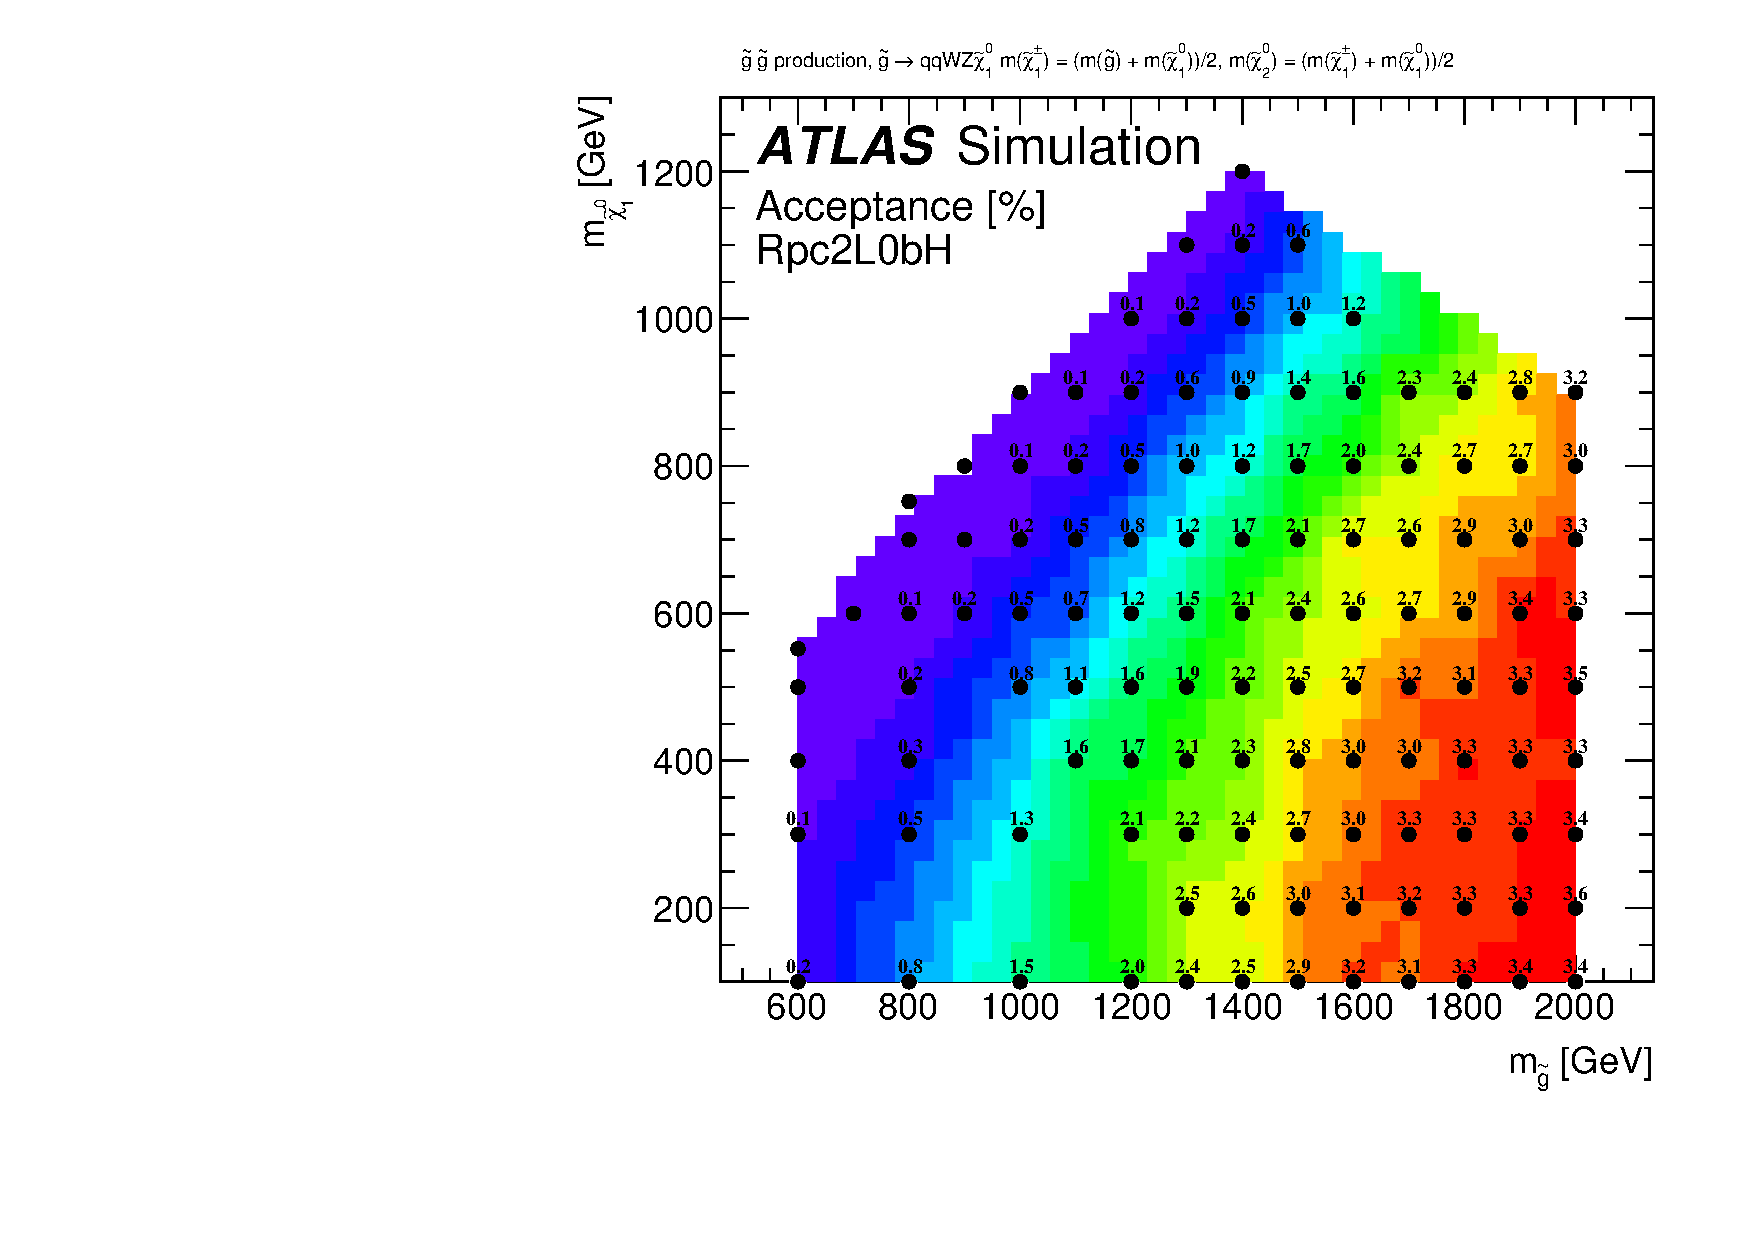
\includegraphics[width=\textwidth]{EffAcc/acceptance_2StepRpc2L0bH}\caption{Rpc2L0bH acceptance}\end{subfigure}
\begin{subfigure}[t]{0.49\textwidth}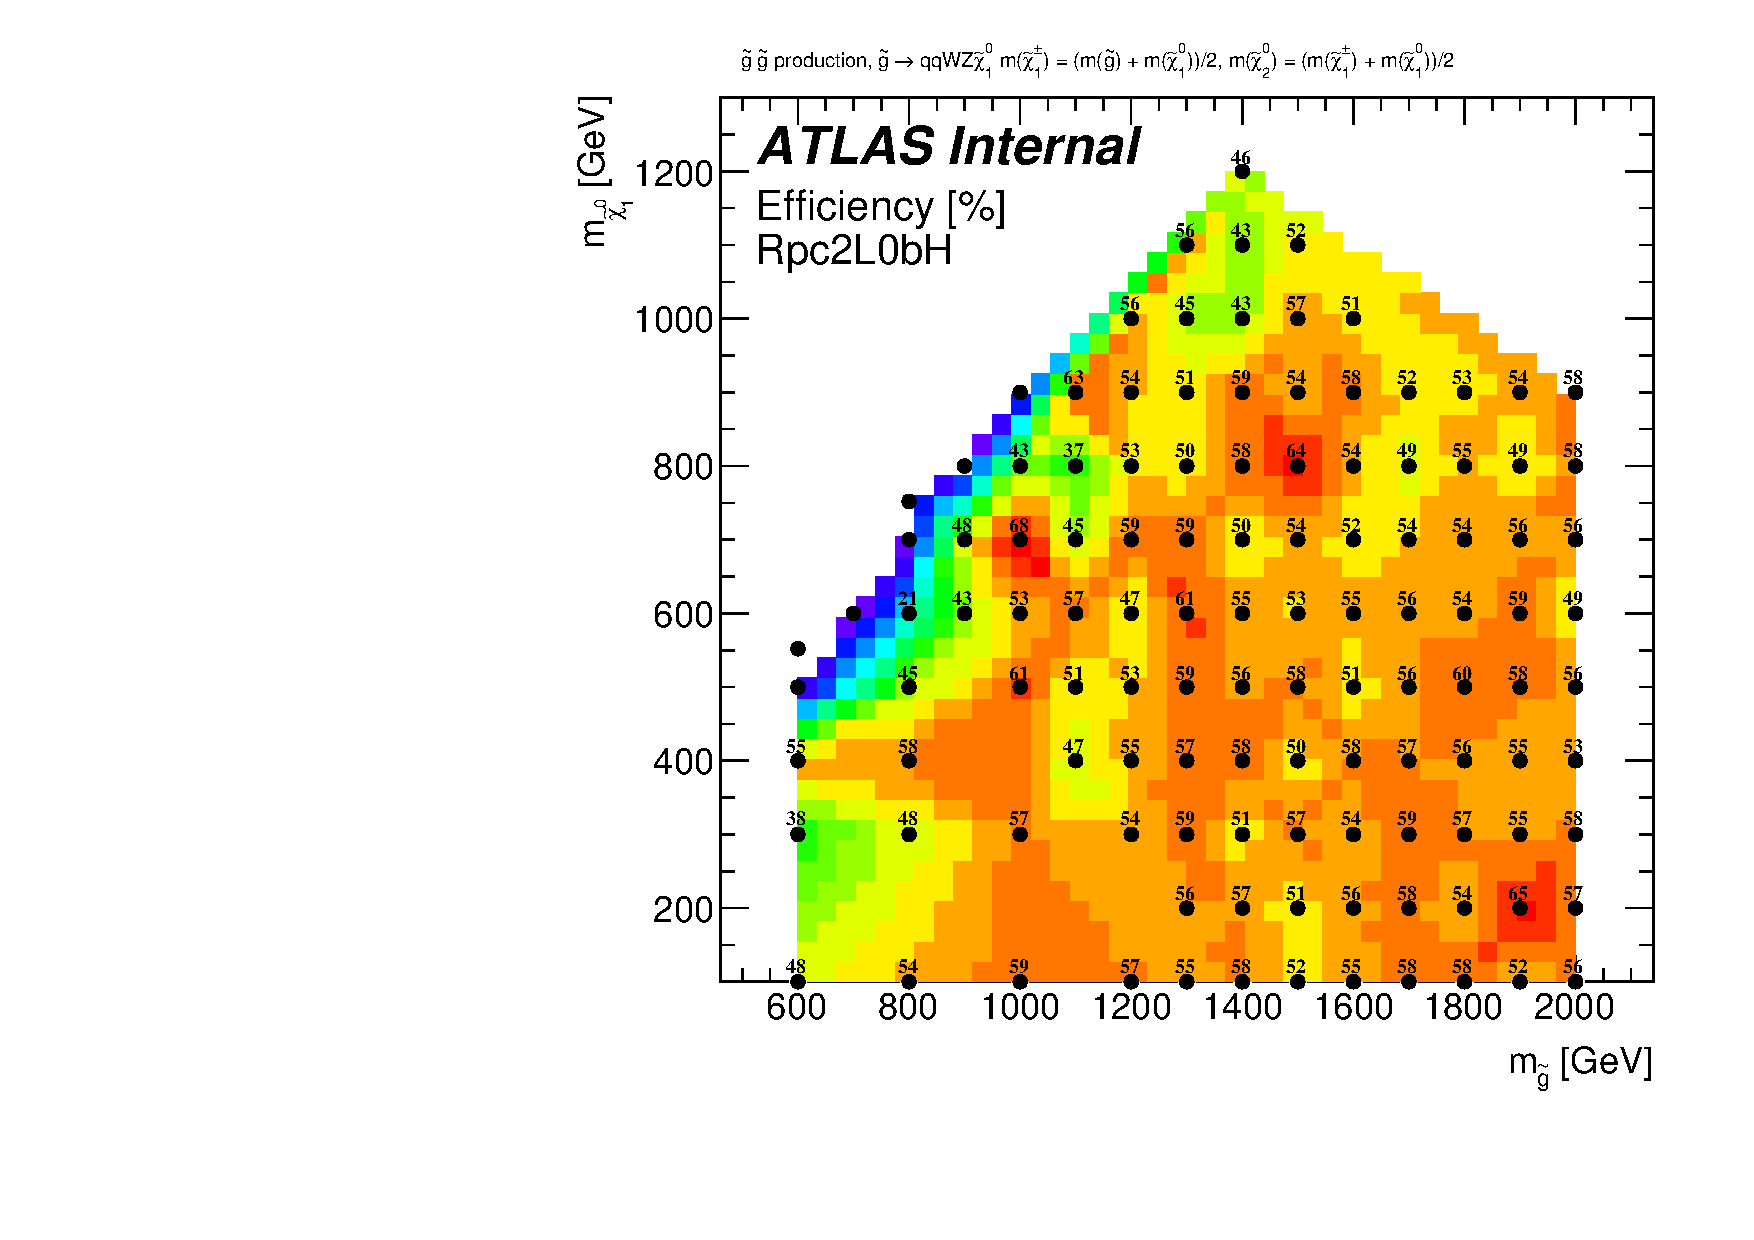
\includegraphics[width=\textwidth]{EffAcc/efficiency_2StepRpc2L0bH}\caption{Rpc2L0bH efficiency}\end{subfigure}
\begin{subfigure}[t]{0.49\textwidth}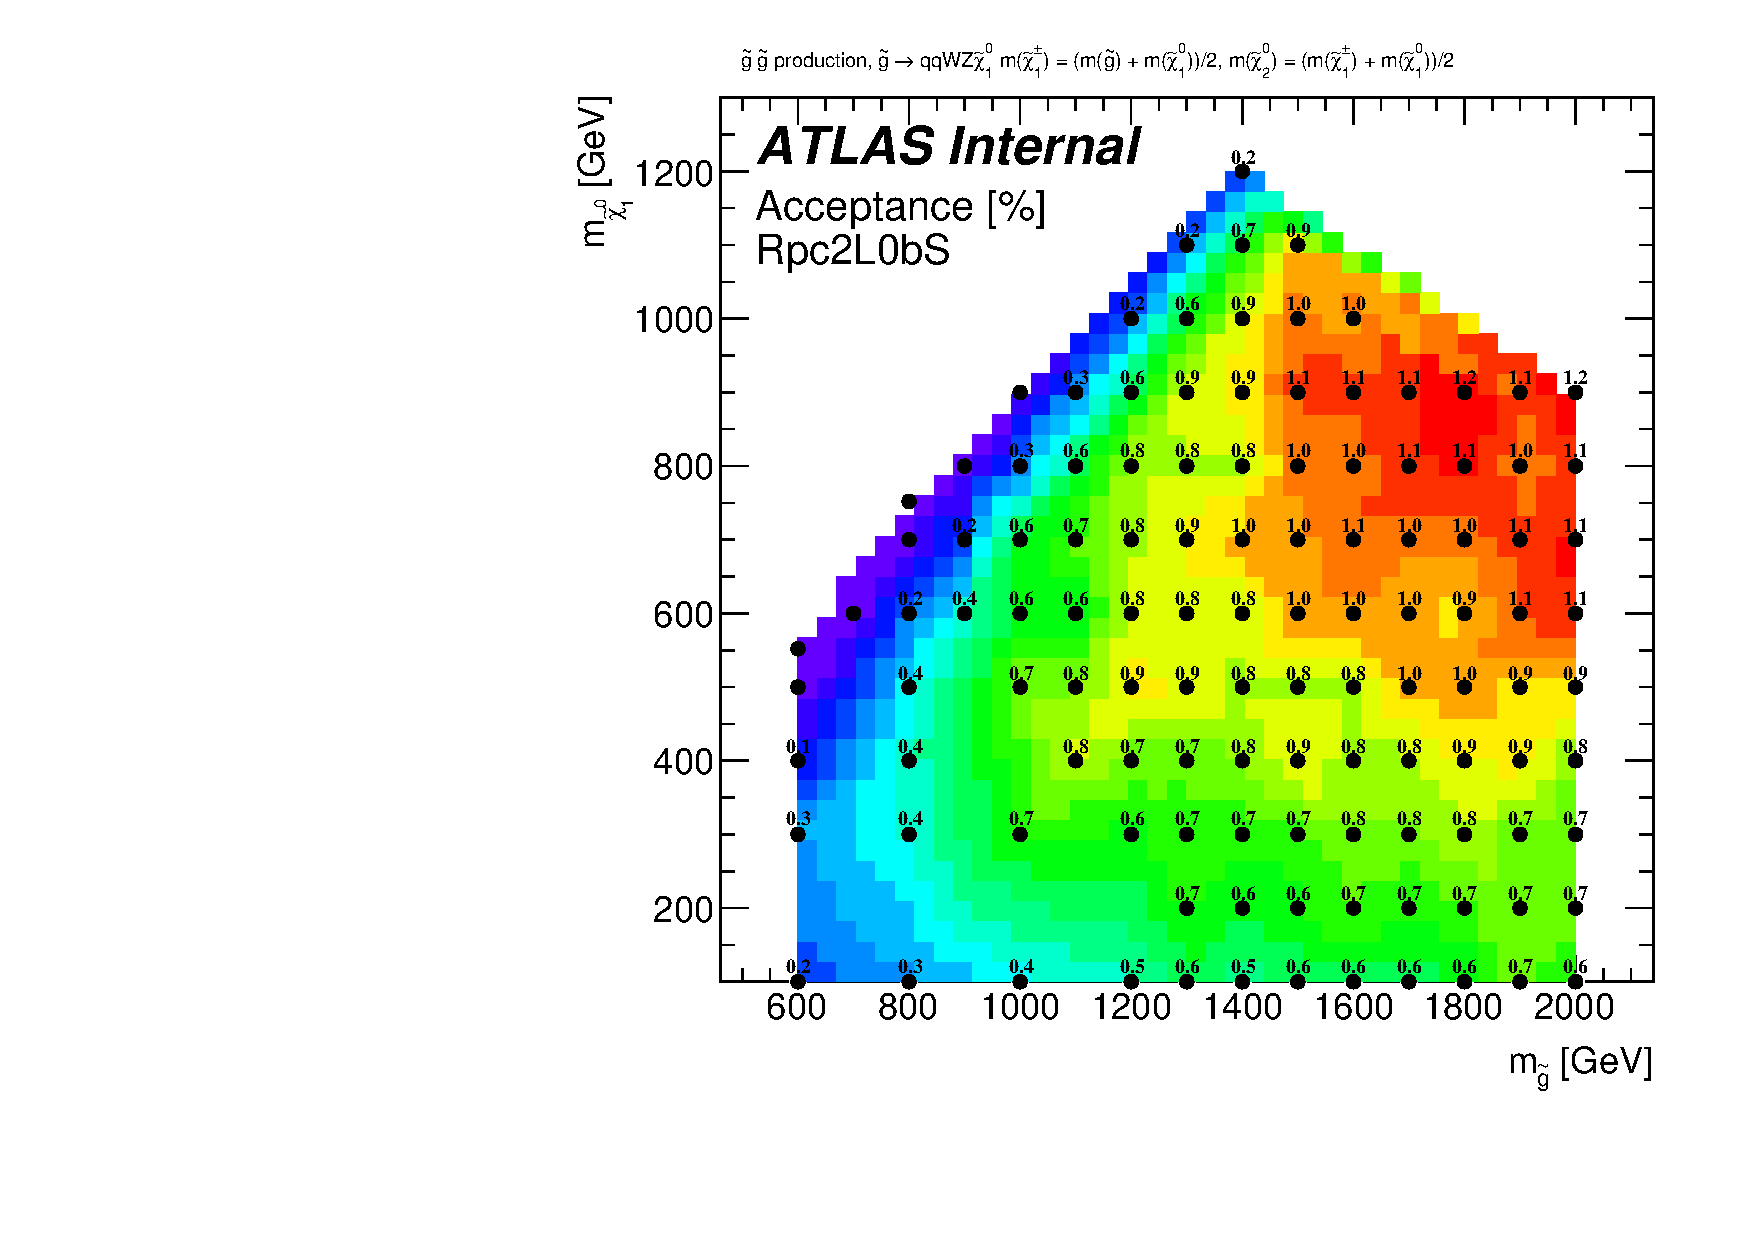
\includegraphics[width=\textwidth]{EffAcc/acceptance_2StepRpc2L0bS}\caption{Rpc2L0bS acceptance}\end{subfigure}
\begin{subfigure}[t]{0.49\textwidth}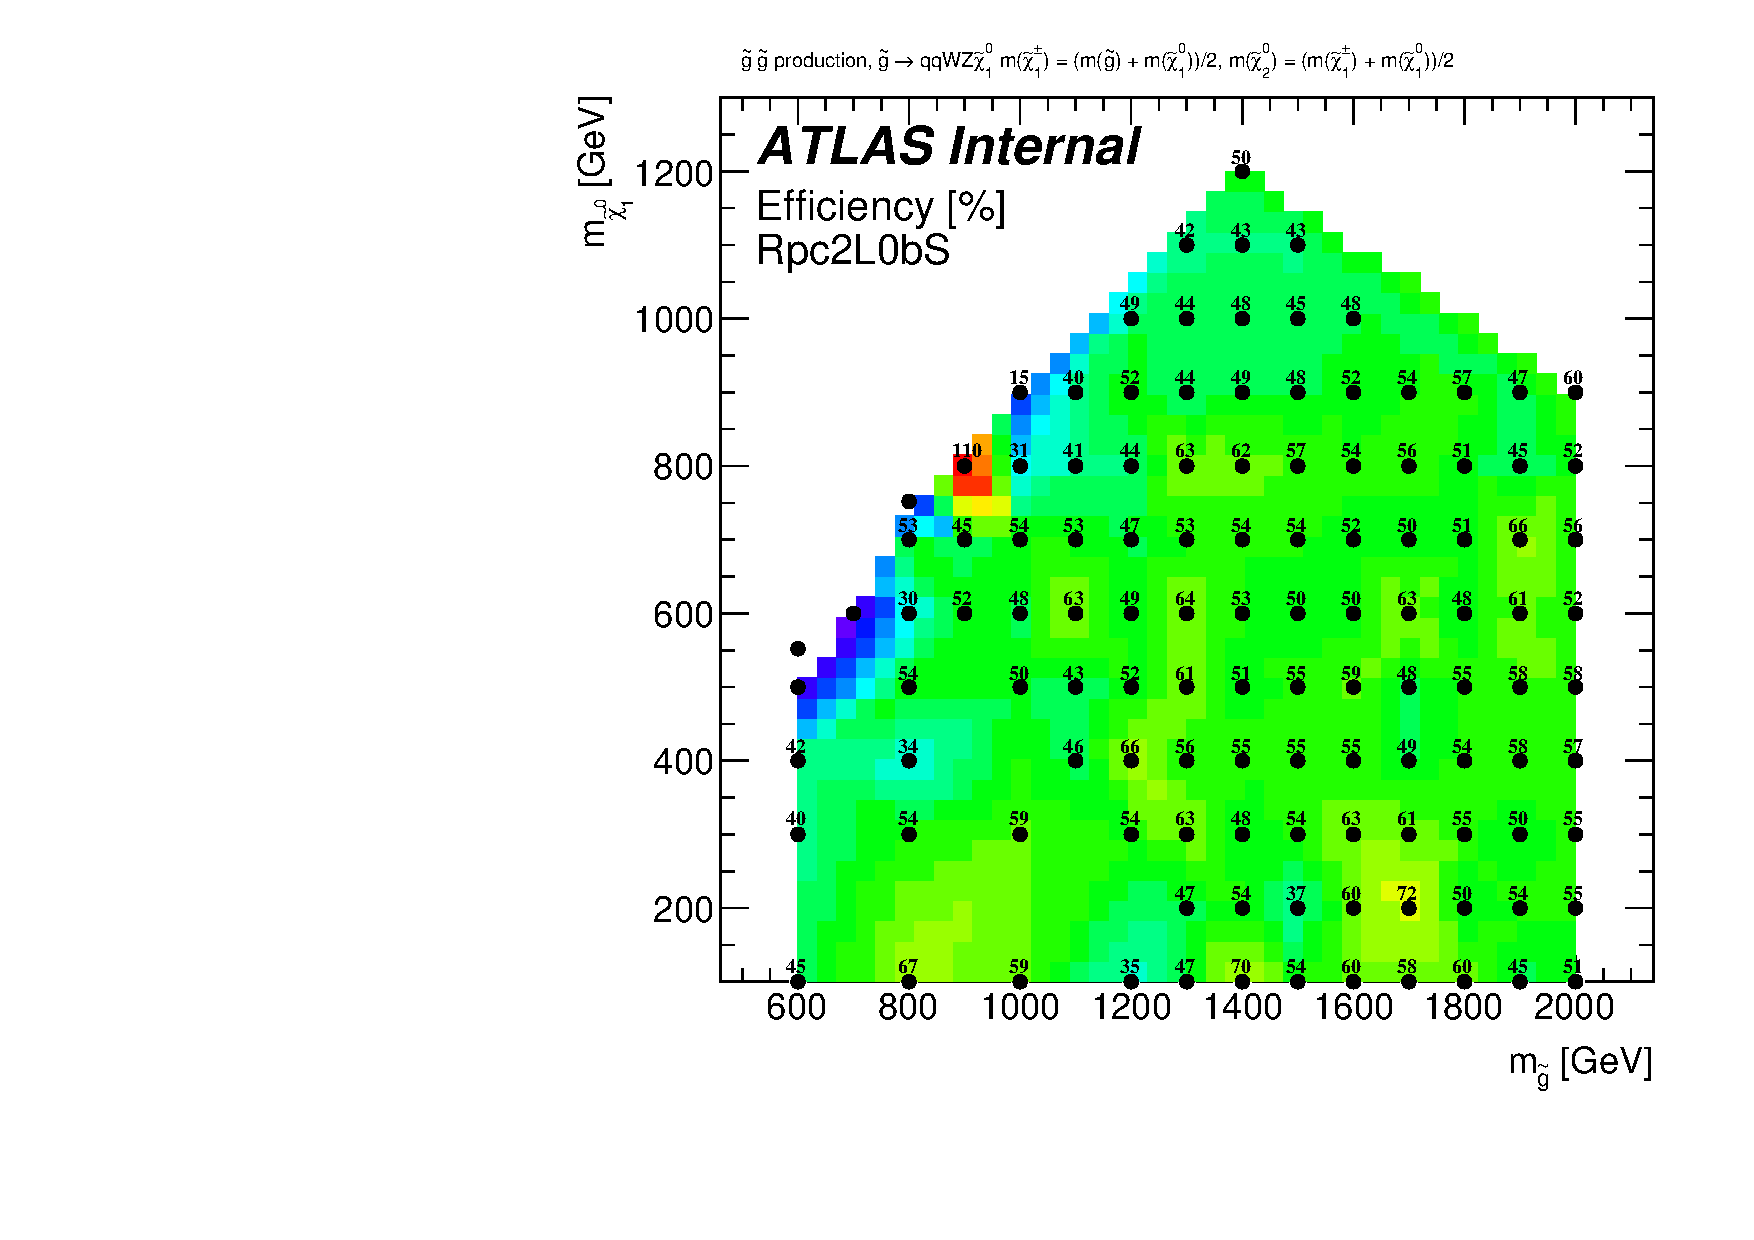
\includegraphics[width=\textwidth]{EffAcc/efficiency_2StepRpc2L0bS}\caption{Rpc2L0bS efficiency}\end{subfigure}
\caption{Signal acceptance (a,c) and reconstruction efficiency (b,d) 
for simplified models of $\gluino\gluino$ production with $\gluino\to q\bar q^{'}WZ\ninoone$ decays, 
in the signal regions Rpc2L0bH (a,b) and Rpc2L0bS (c,d).}
\end{figure}

\begin{figure}[htb!]
\centering
\begin{subfigure}[t]{0.49\textwidth}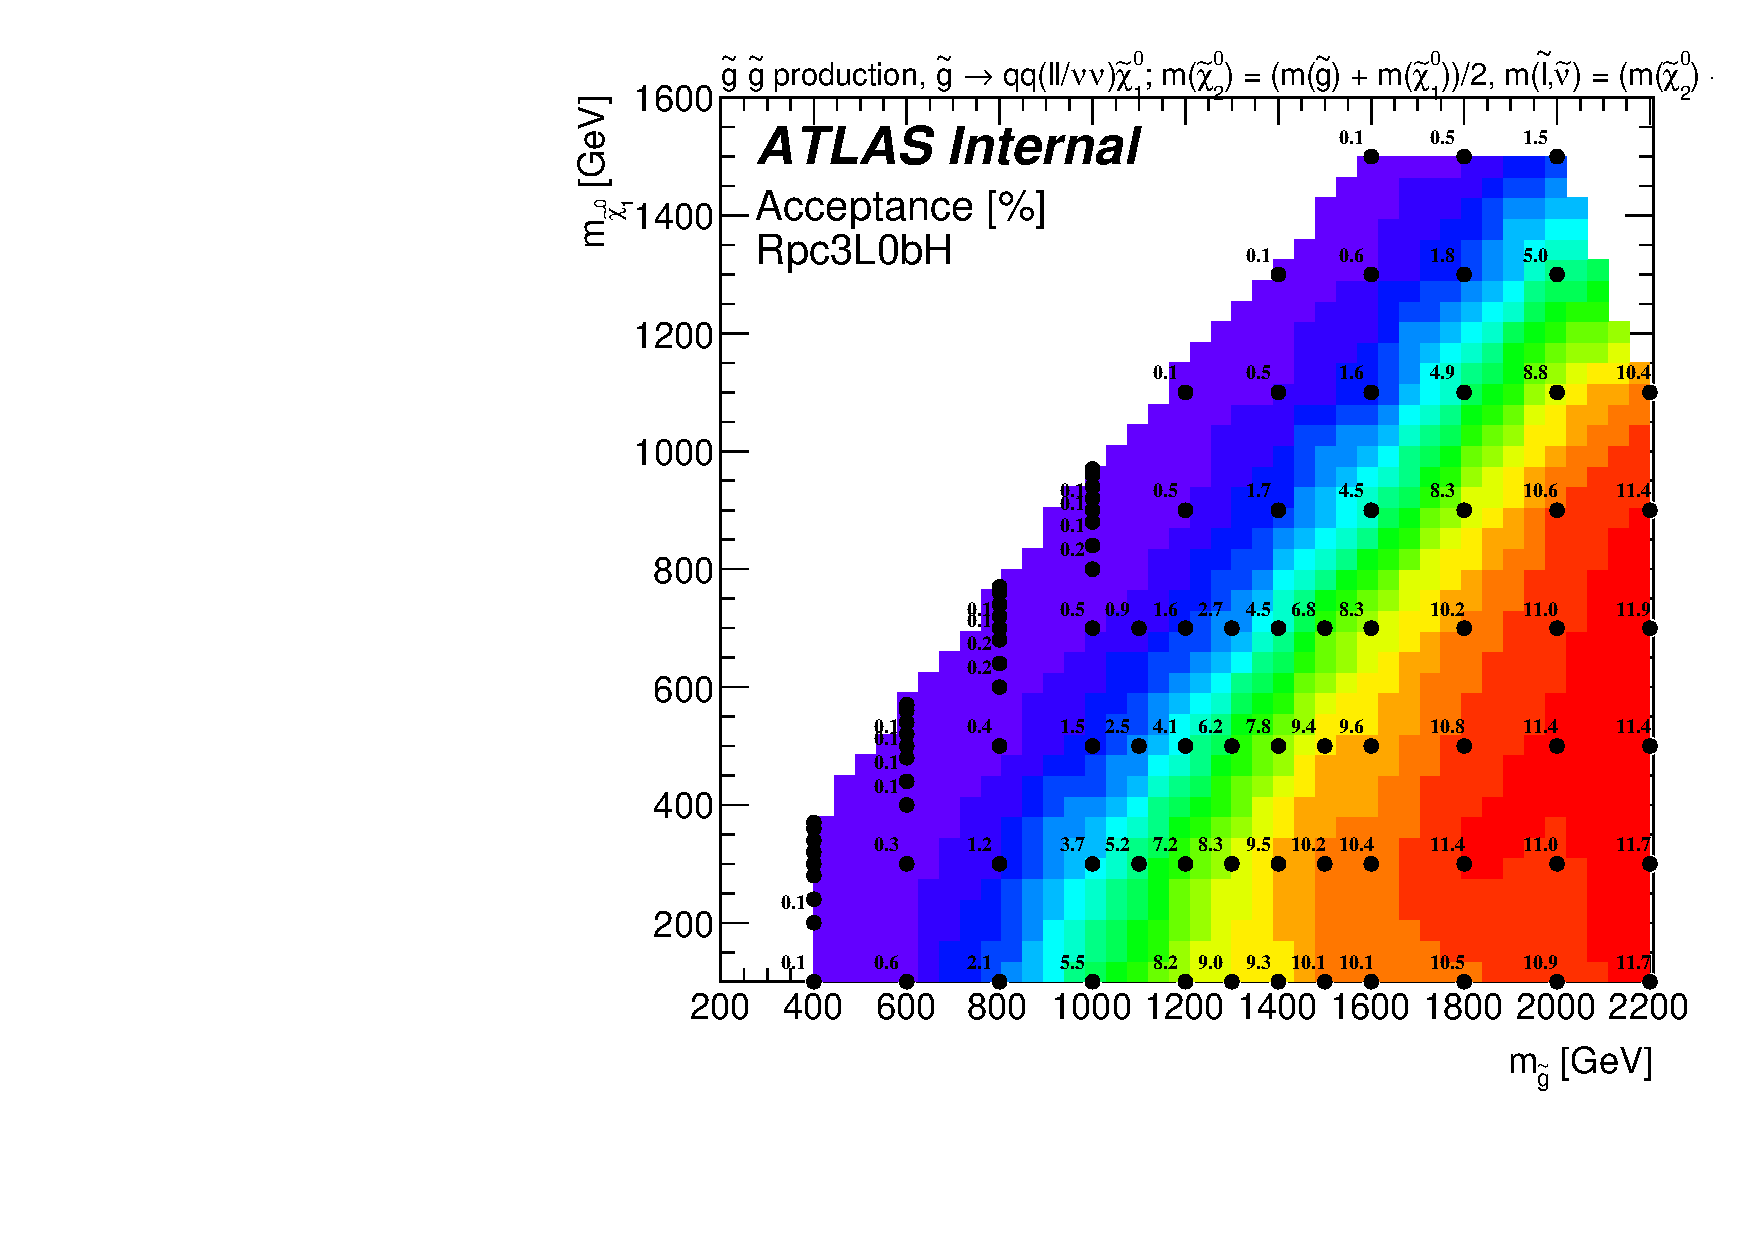
\includegraphics[width=\textwidth]{EffAcc/acceptance_GSLRpc3L0bH}\caption{Rpc3L0bH acceptance}\end{subfigure}
\begin{subfigure}[t]{0.49\textwidth}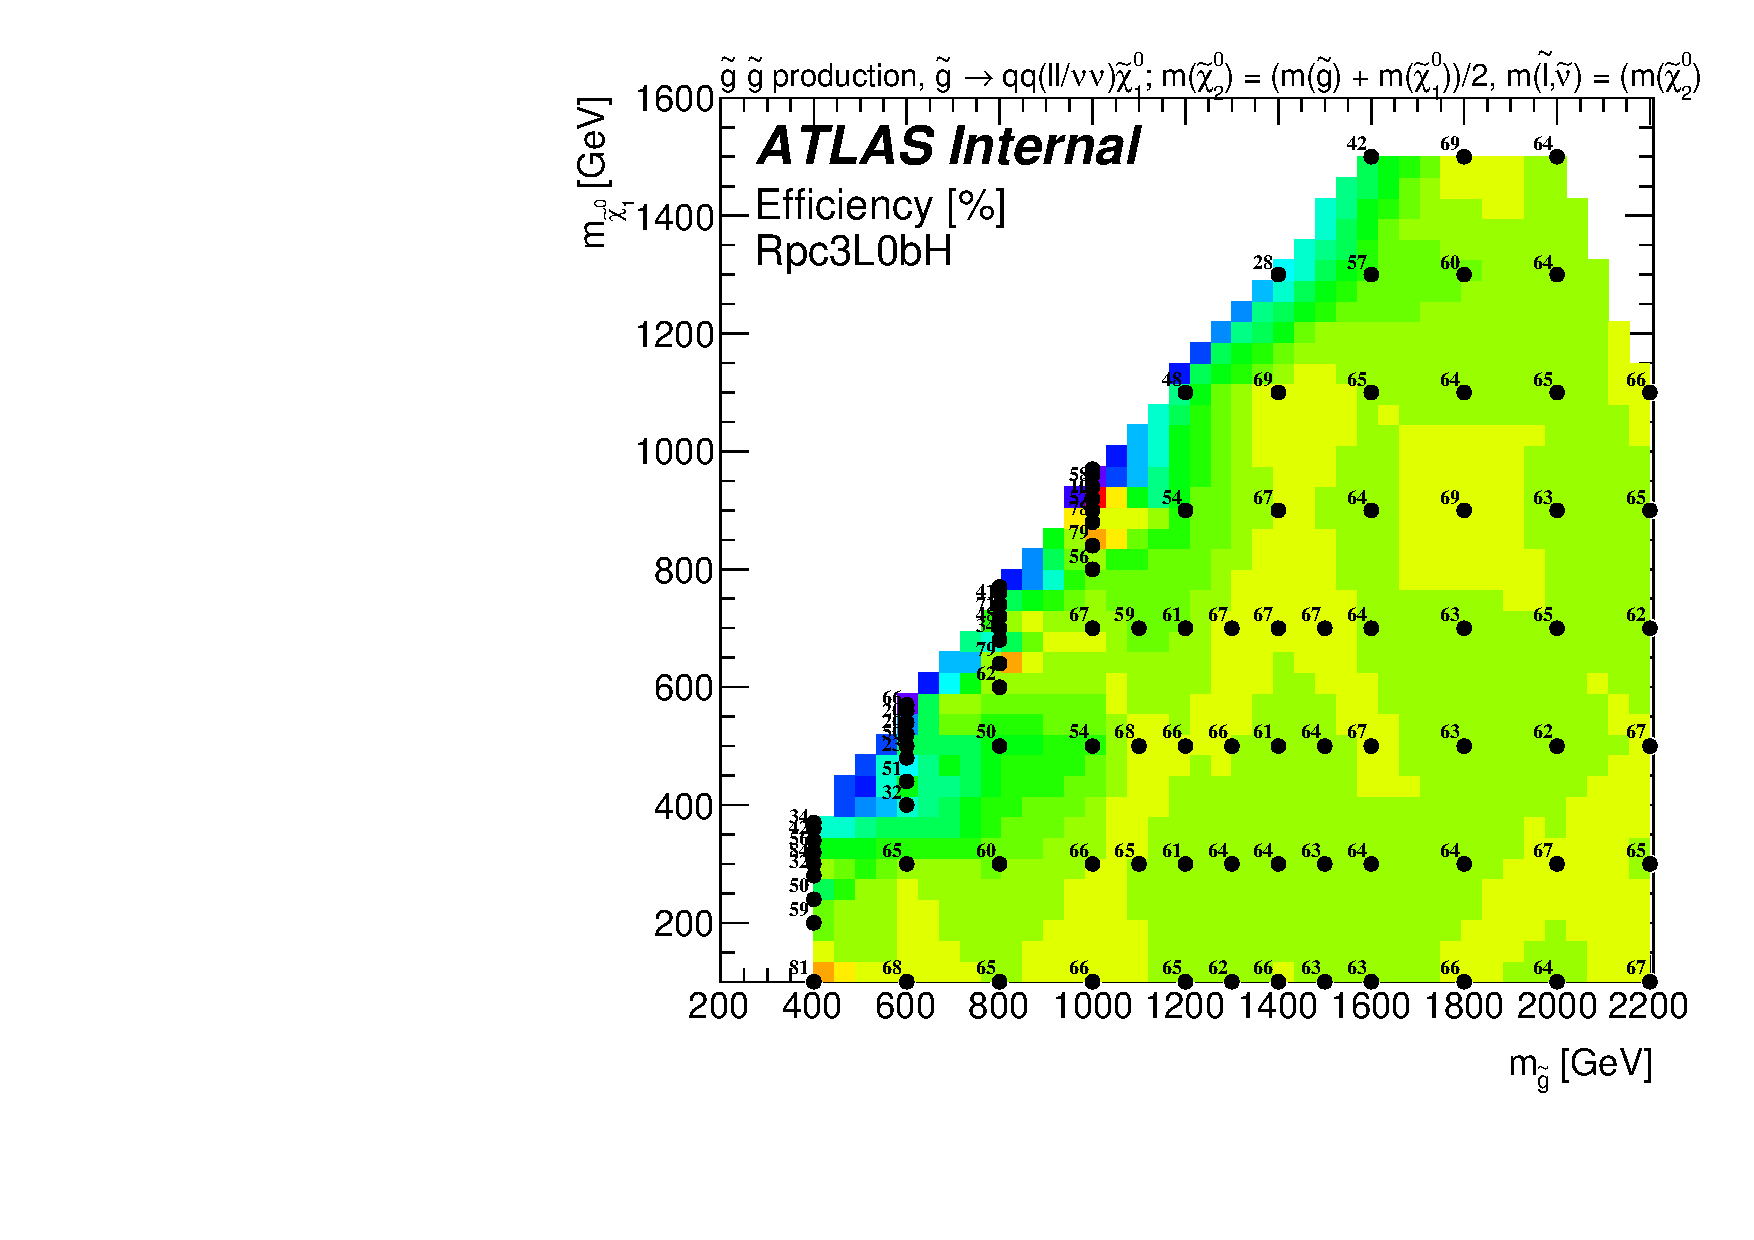
\includegraphics[width=\textwidth]{EffAcc/efficiency_GSLRpc3L0bH}\caption{Rpc3L0bH efficiency}\end{subfigure}
\begin{subfigure}[t]{0.49\textwidth}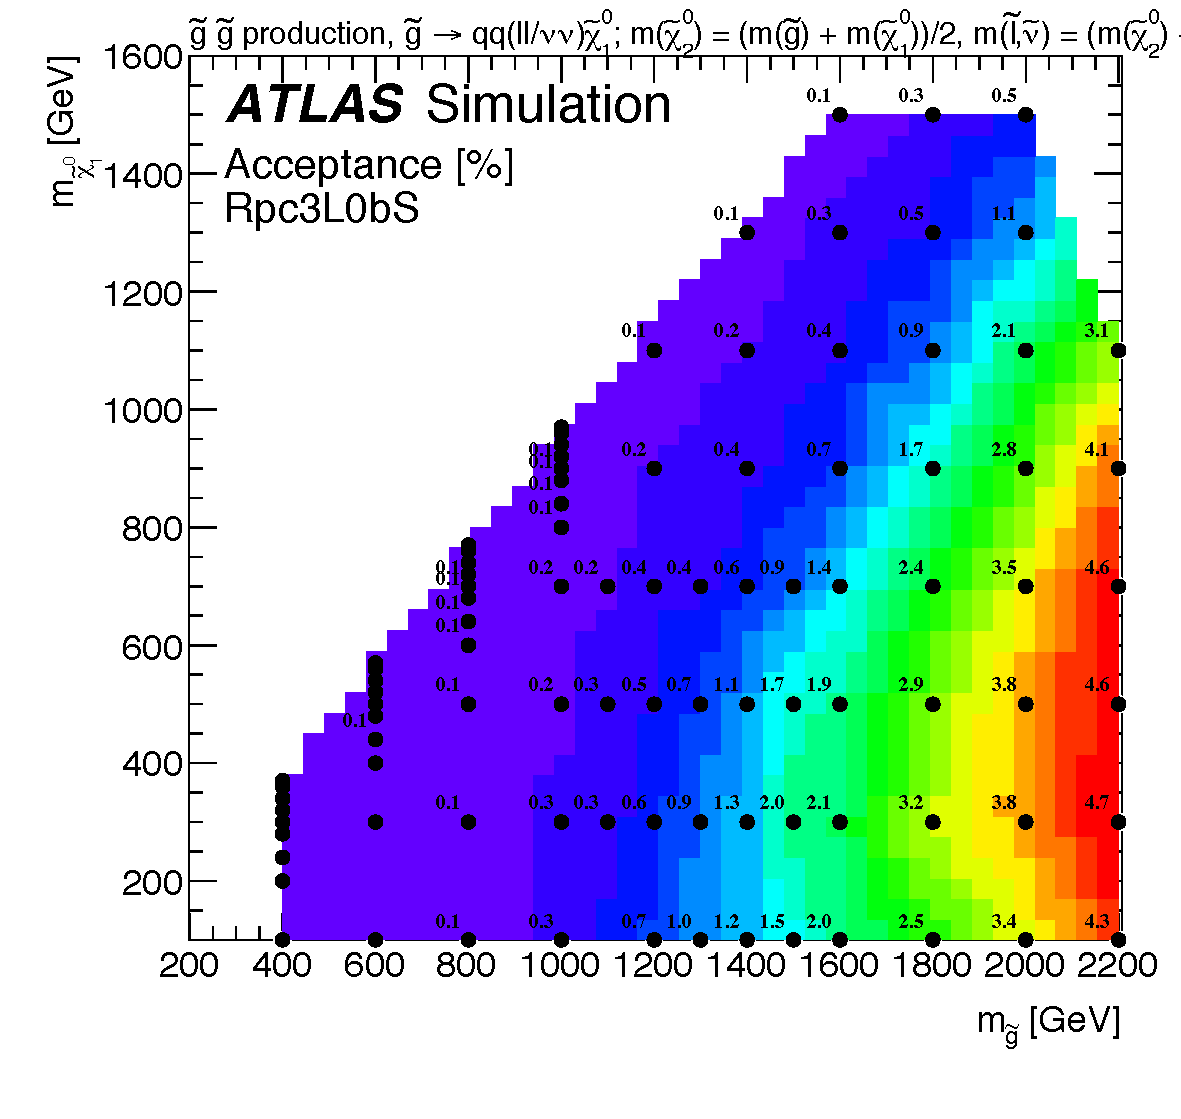
\includegraphics[width=\textwidth]{EffAcc/acceptance_GSLRpc3L0bS}\caption{Rpc3L0bS acceptance}\end{subfigure}
\begin{subfigure}[t]{0.49\textwidth}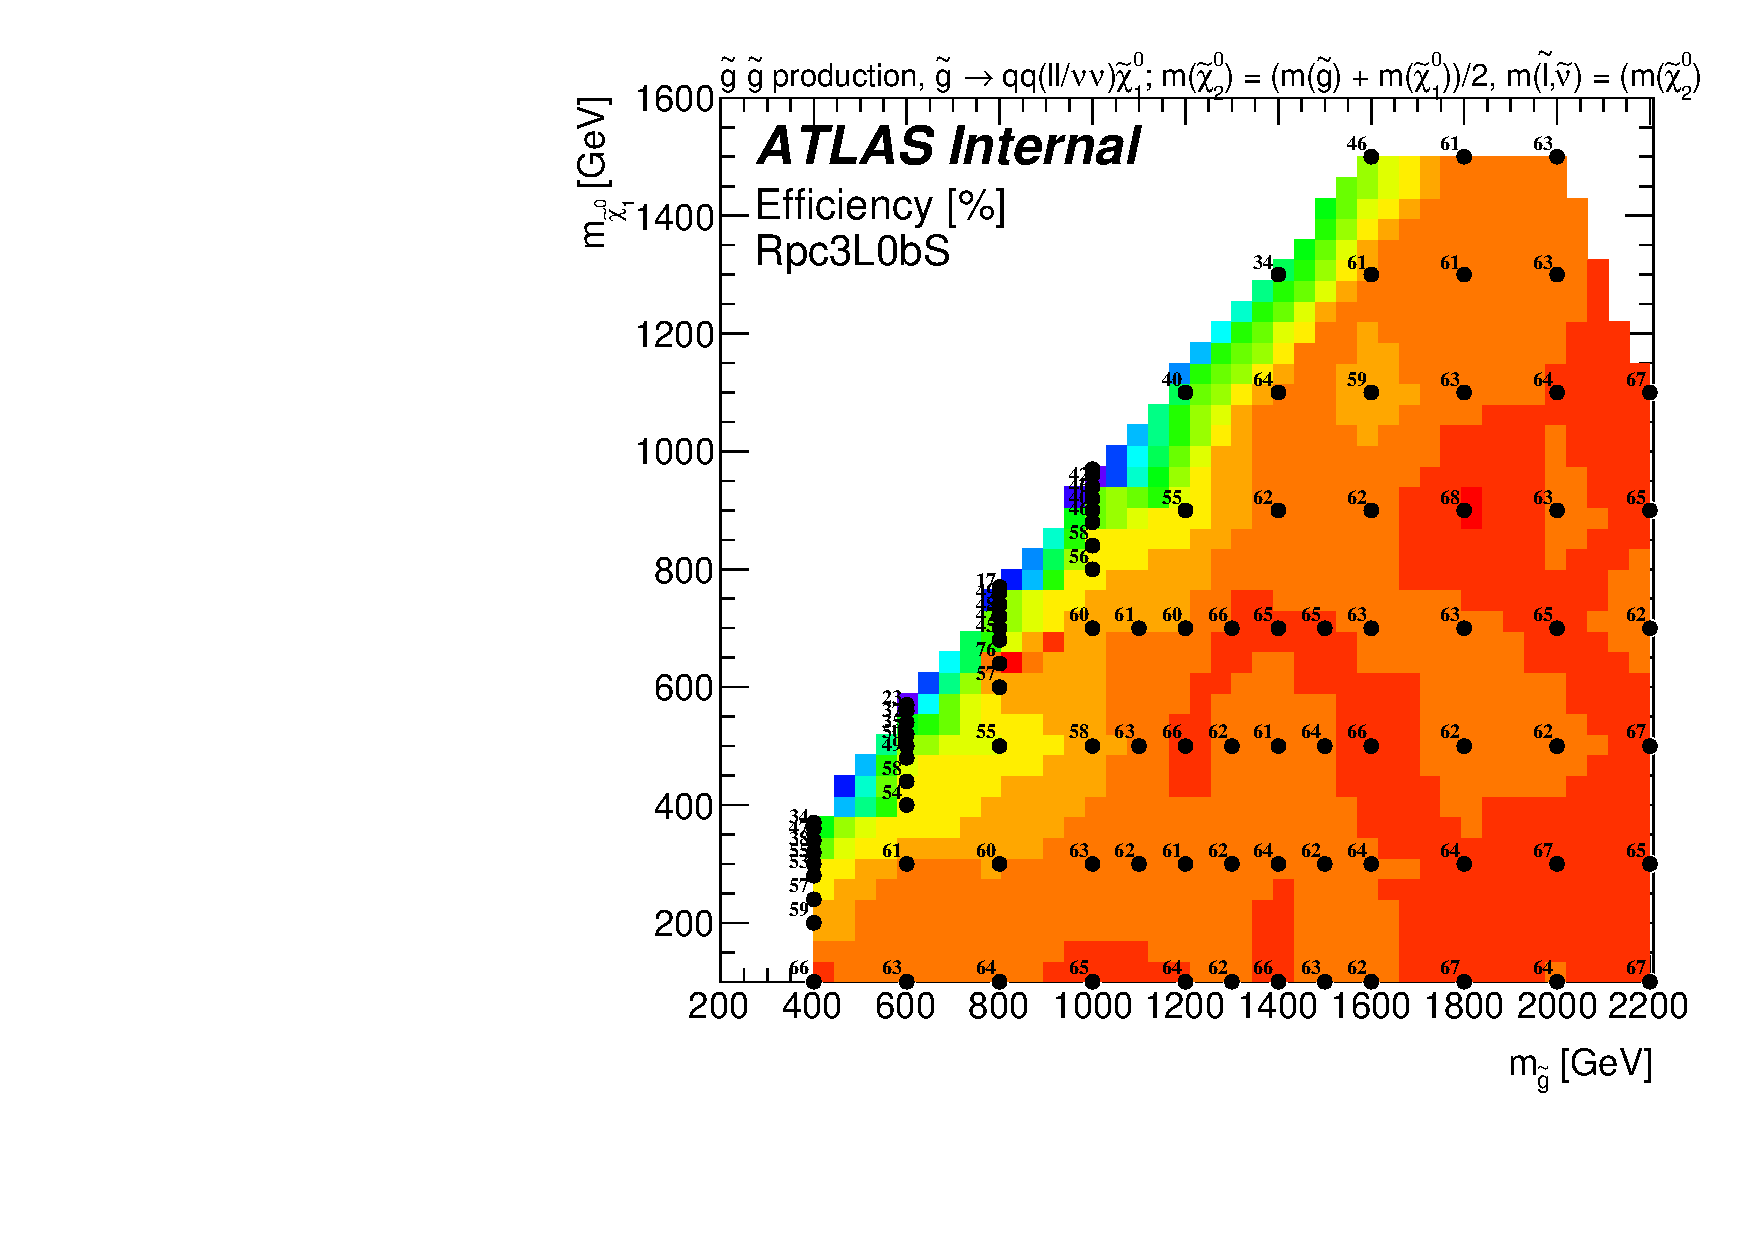
\includegraphics[width=\textwidth]{EffAcc/efficiency_GSLRpc3L0bS}\caption{Rpc3L0bS efficiency}\end{subfigure}
\caption{Signal acceptance (a,c) and reconstruction efficiency (b,d) 
for simplified models of $\gluino\gluino$ production with $\gluino\to q\bar q(\ell\ell/\nu\nu)\ninoone$ decays, 
in the signal regions Rpc3L0bH (a,b) and Rpc3L0bS (c,d).}
\end{figure}

\begin{figure}[htb!]
\centering
\begin{subfigure}[t]{0.49\textwidth}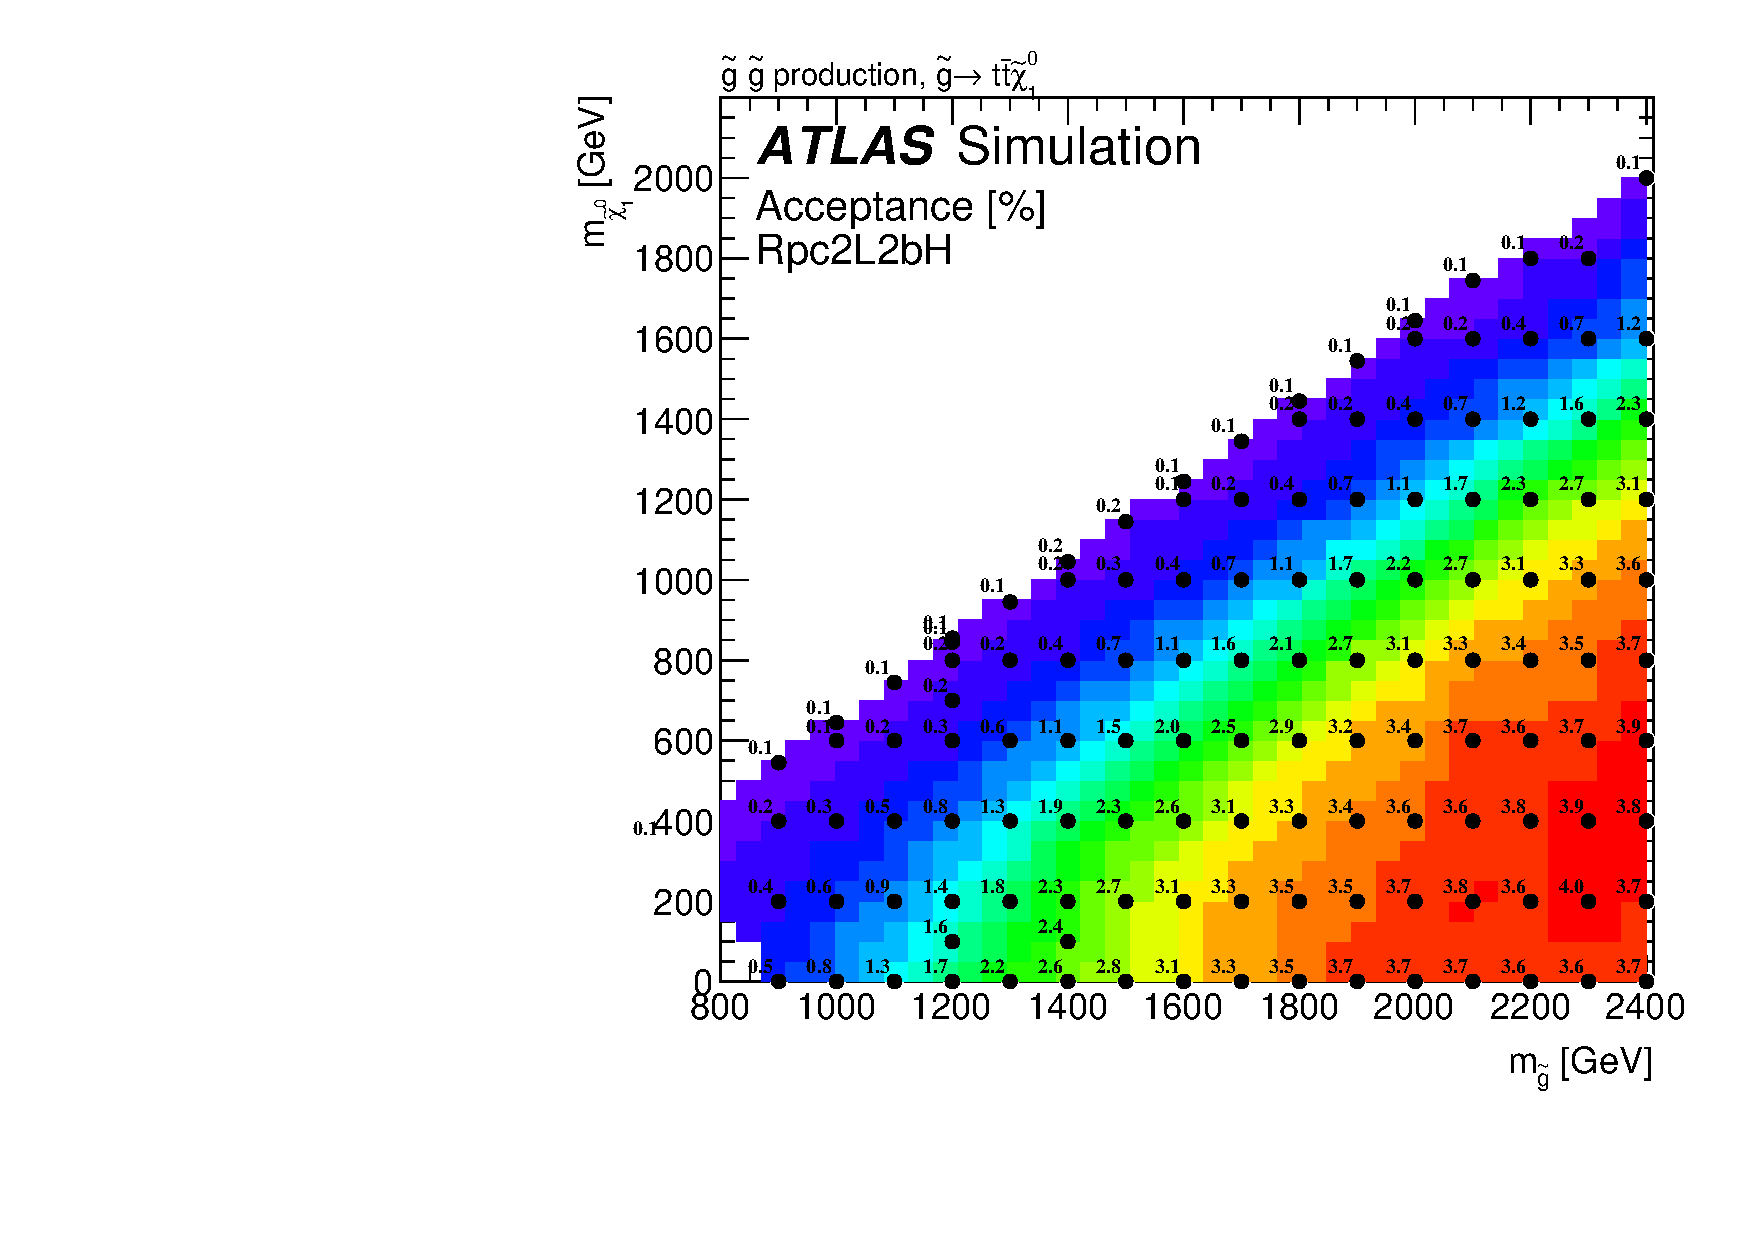
\includegraphics[width=\textwidth]{EffAcc/acceptance_GttRpc2L2bH}\caption{Rpc2L2bH acceptance}\end{subfigure}
\begin{subfigure}[t]{0.49\textwidth}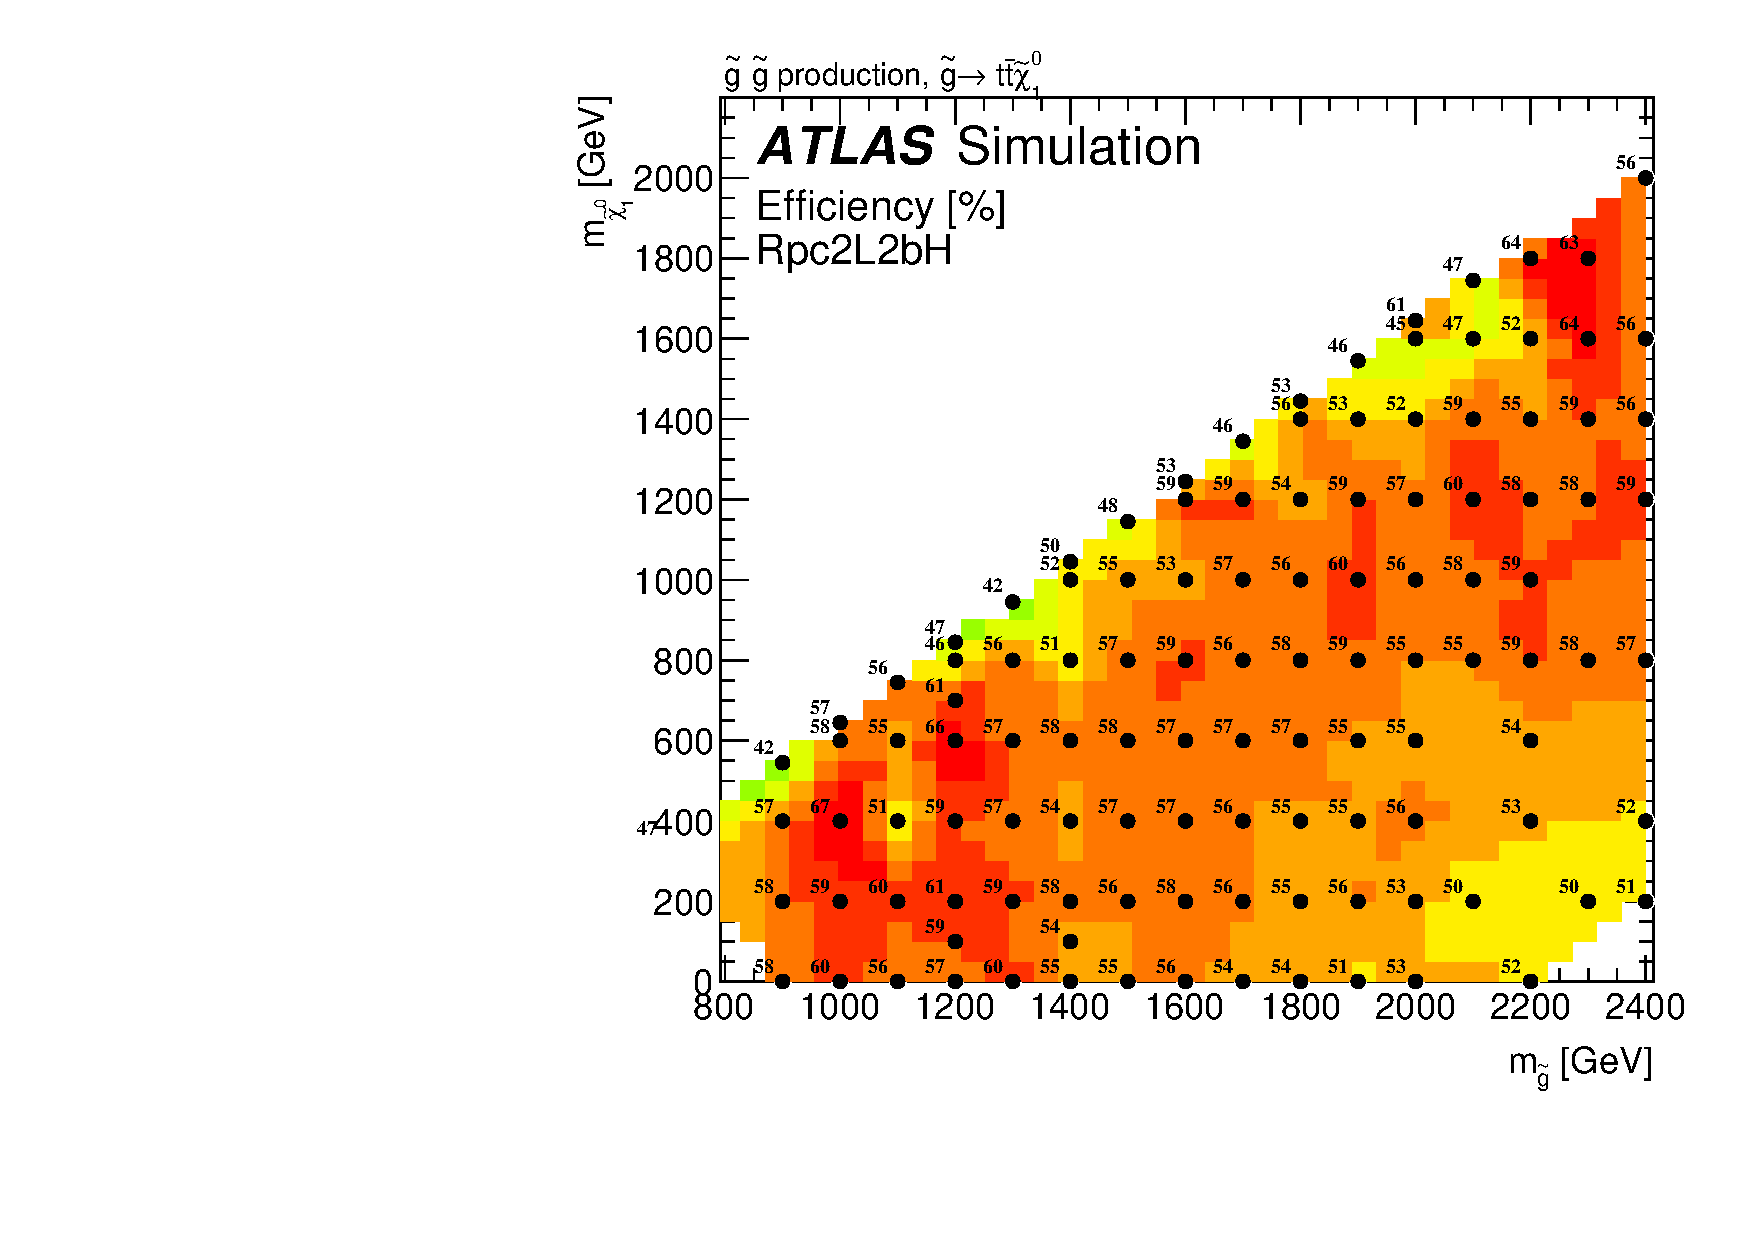
\includegraphics[width=\textwidth]{EffAcc/efficiency_GttRpc2L2bH}\caption{Rpc2L2bH efficiency}\end{subfigure}
\begin{subfigure}[t]{0.49\textwidth}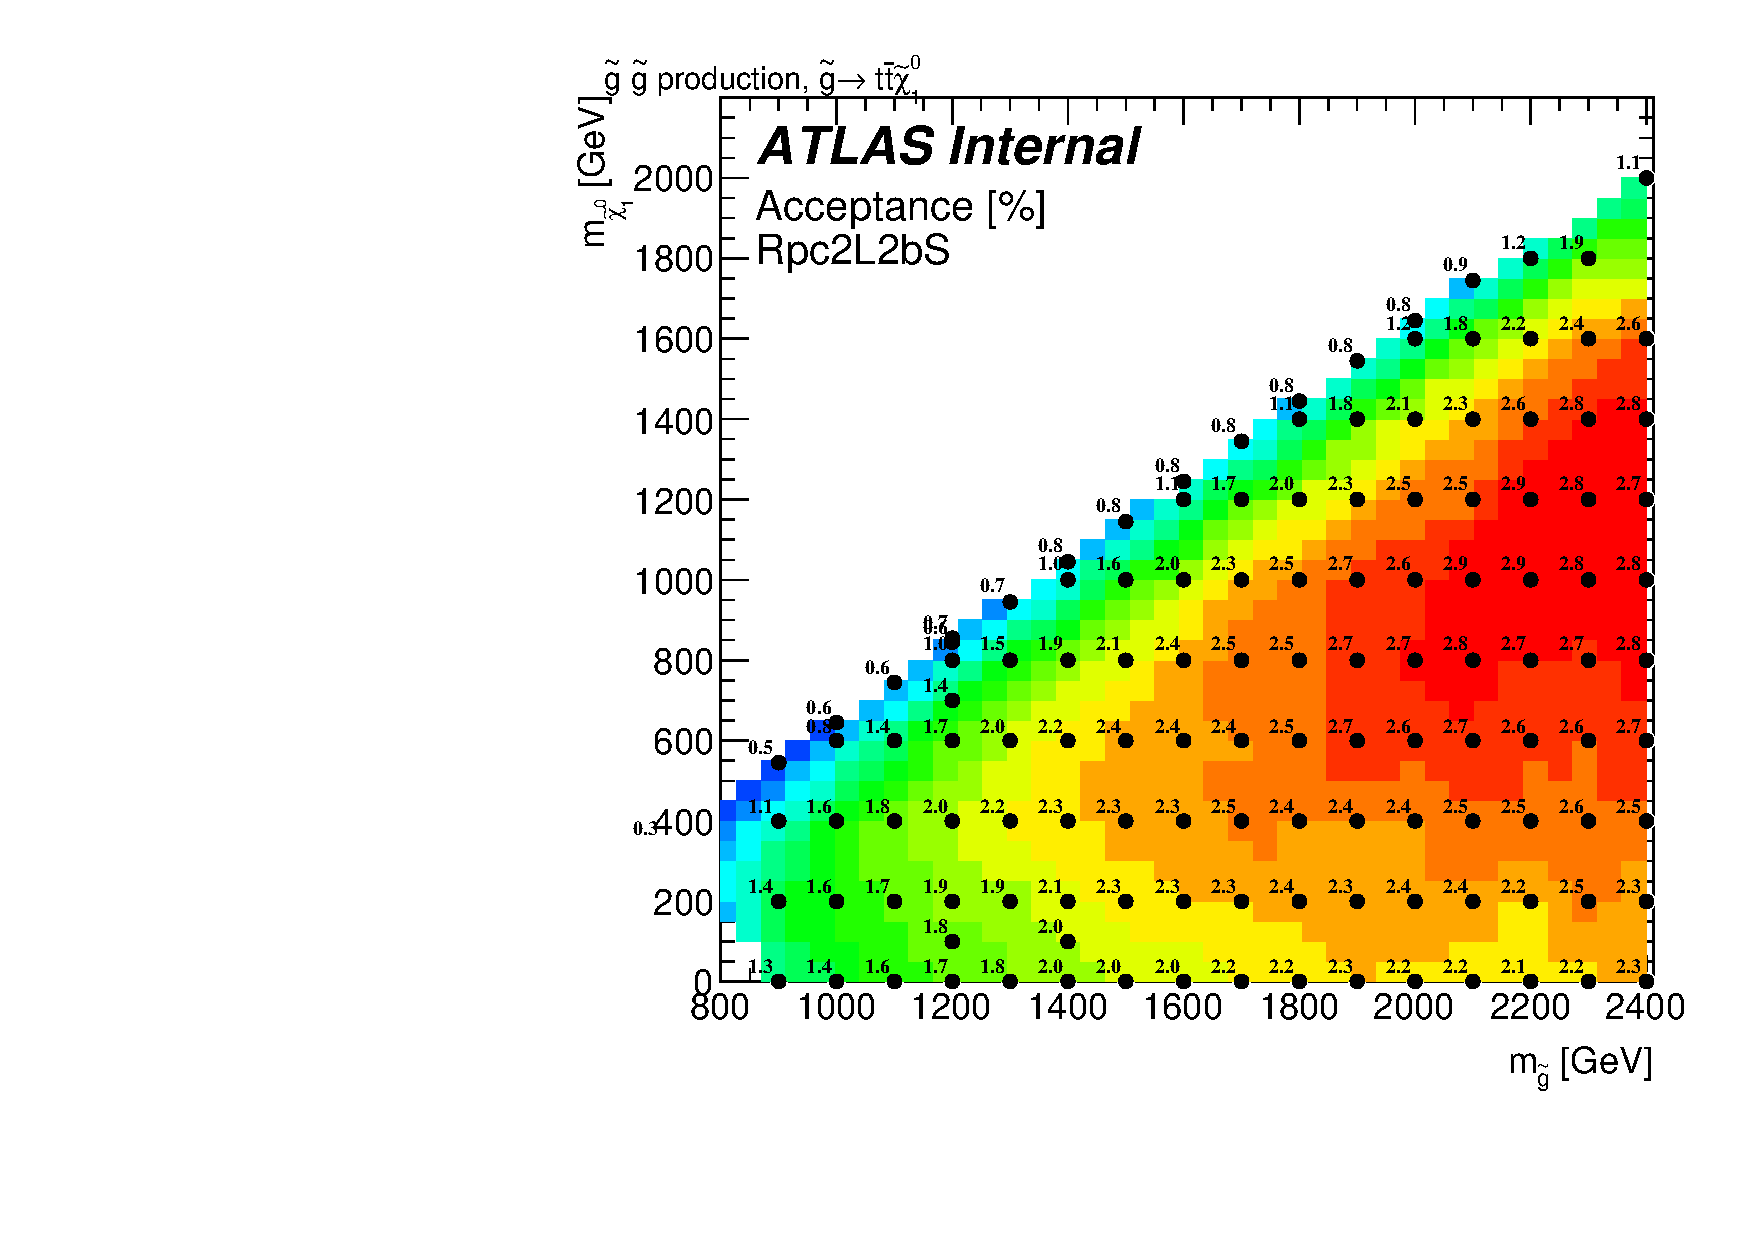
\includegraphics[width=\textwidth]{EffAcc/acceptance_GttRpc2L2bS}\caption{Rpc2L2bS acceptance}\end{subfigure}
\begin{subfigure}[t]{0.49\textwidth}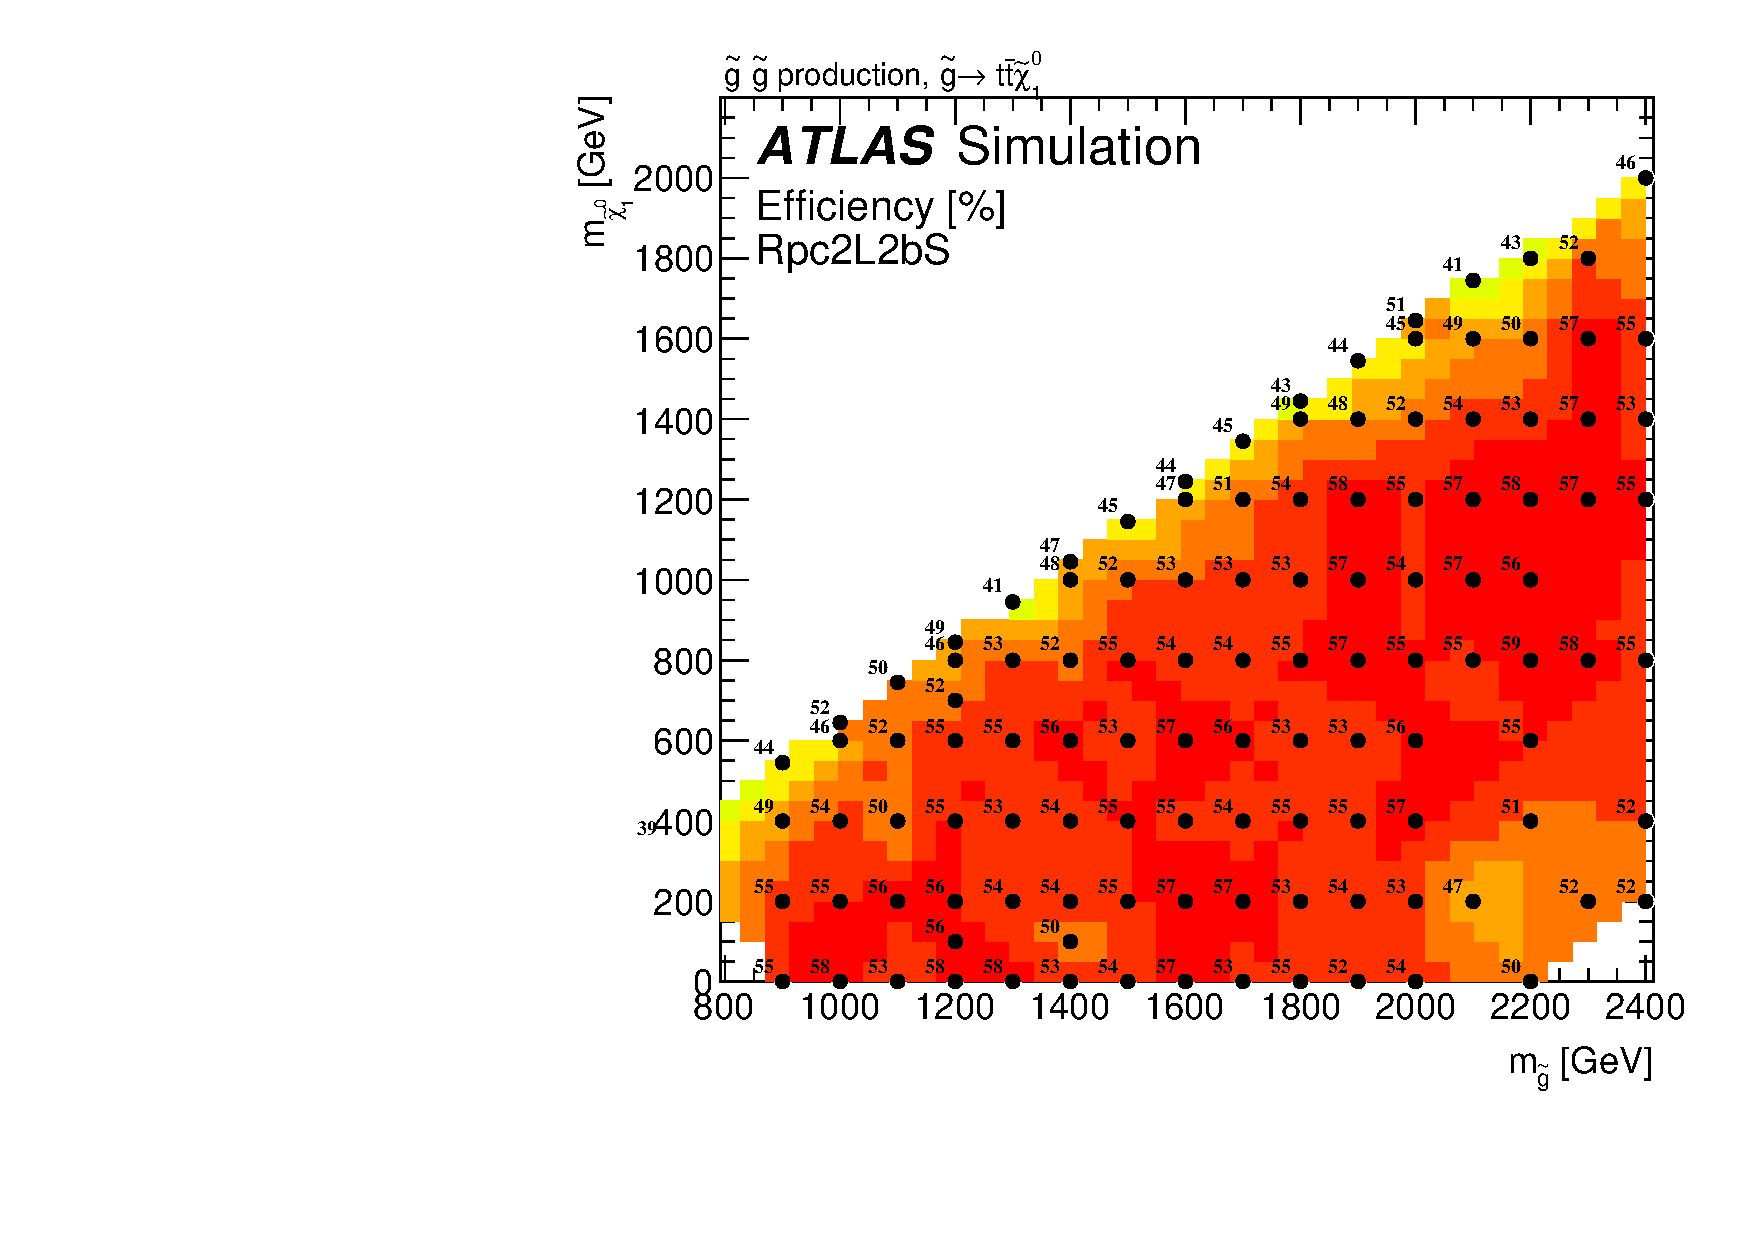
\includegraphics[width=\textwidth]{EffAcc/efficiency_GttRpc2L2bS}\caption{Rpc2L2bS efficiency}\end{subfigure}
\caption{Signal acceptance (a,c) and reconstruction efficiency (b,d) 
for simplified models of $\gluino\gluino$ production with $\gluino\to t\bar t\ninoone$ decays, 
in the signal regions Rpc2L2bH (a,b) and Rpc2L2bS (c,d).}
\end{figure}

\begin{figure}[htb!]
\centering
\begin{subfigure}[t]{0.49\textwidth}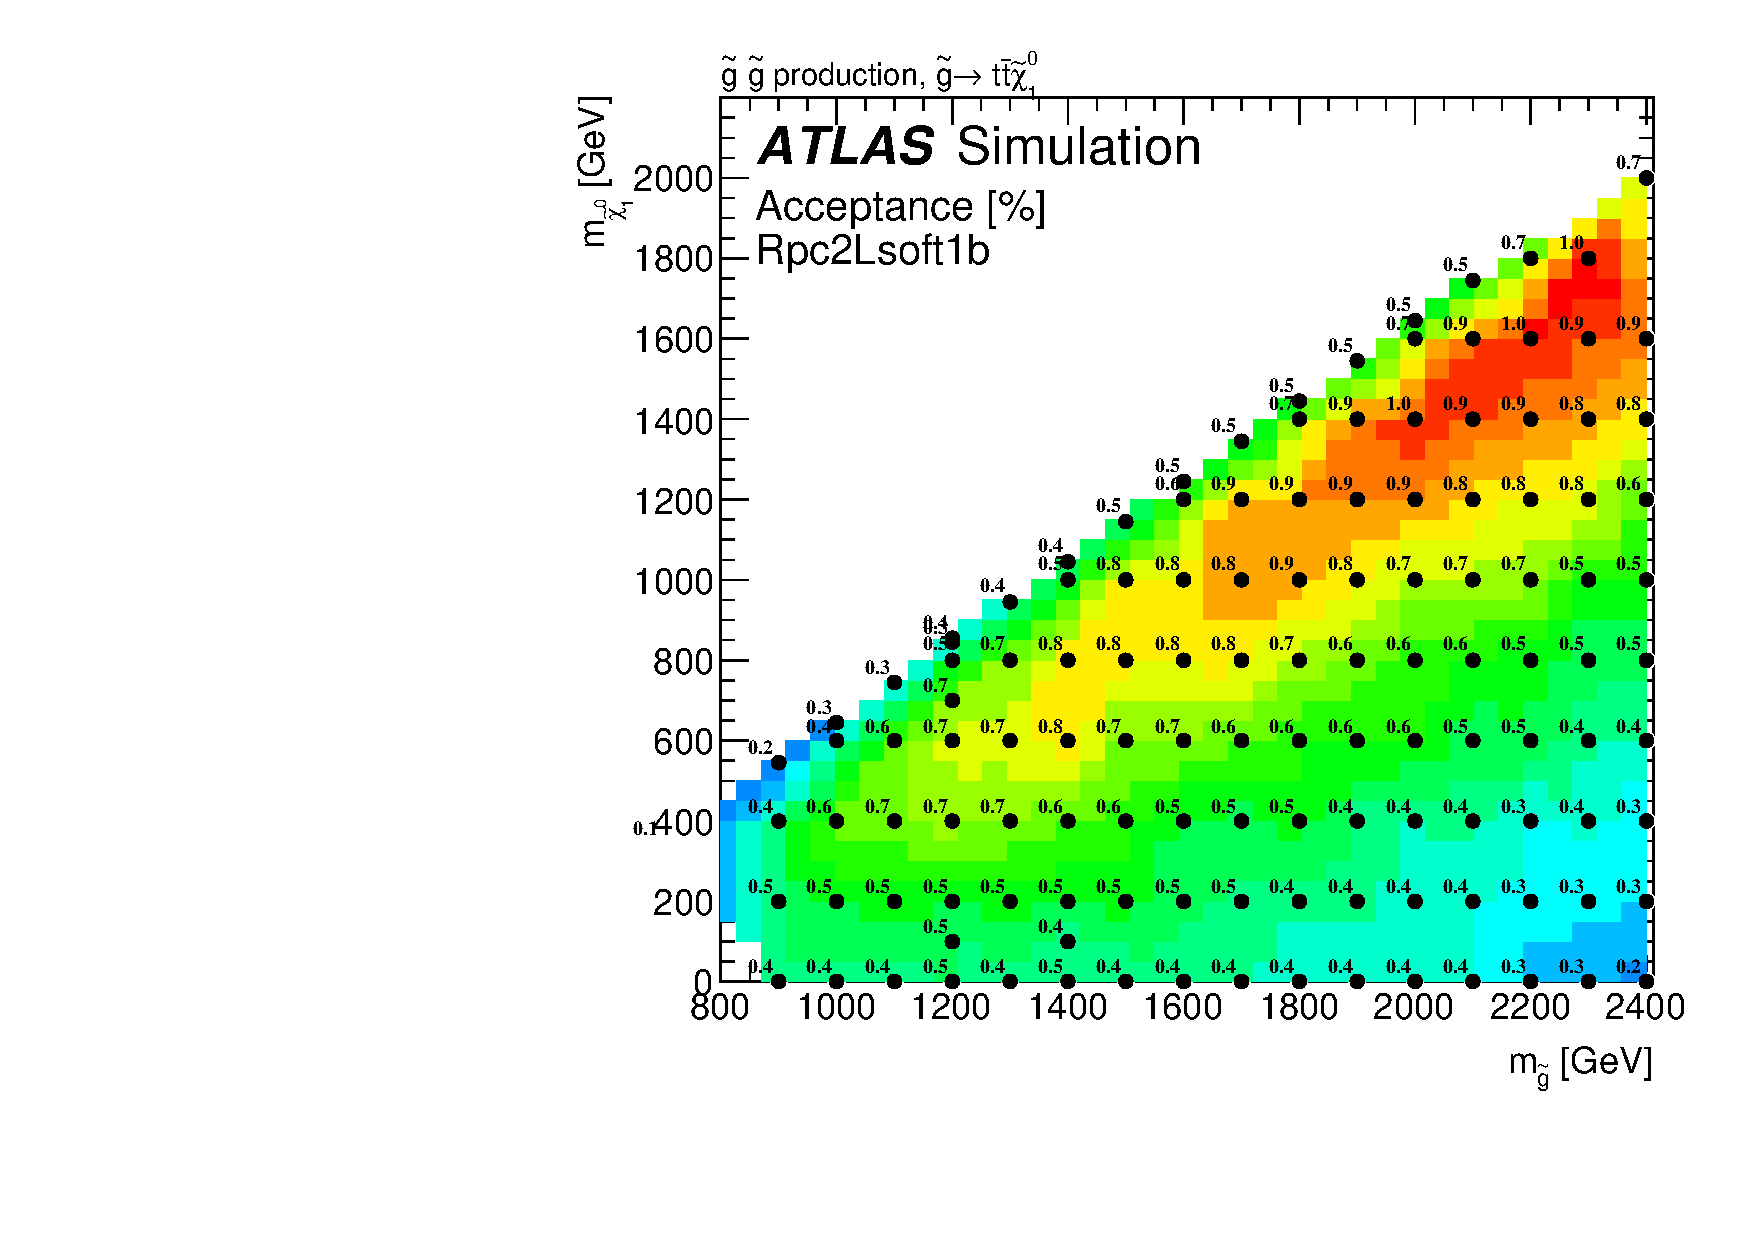
\includegraphics[width=\textwidth]{EffAcc/acceptance_GttRpc2Lsoft1b}\caption{Rpc2Lsoft1b acceptance}\end{subfigure}
\begin{subfigure}[t]{0.49\textwidth}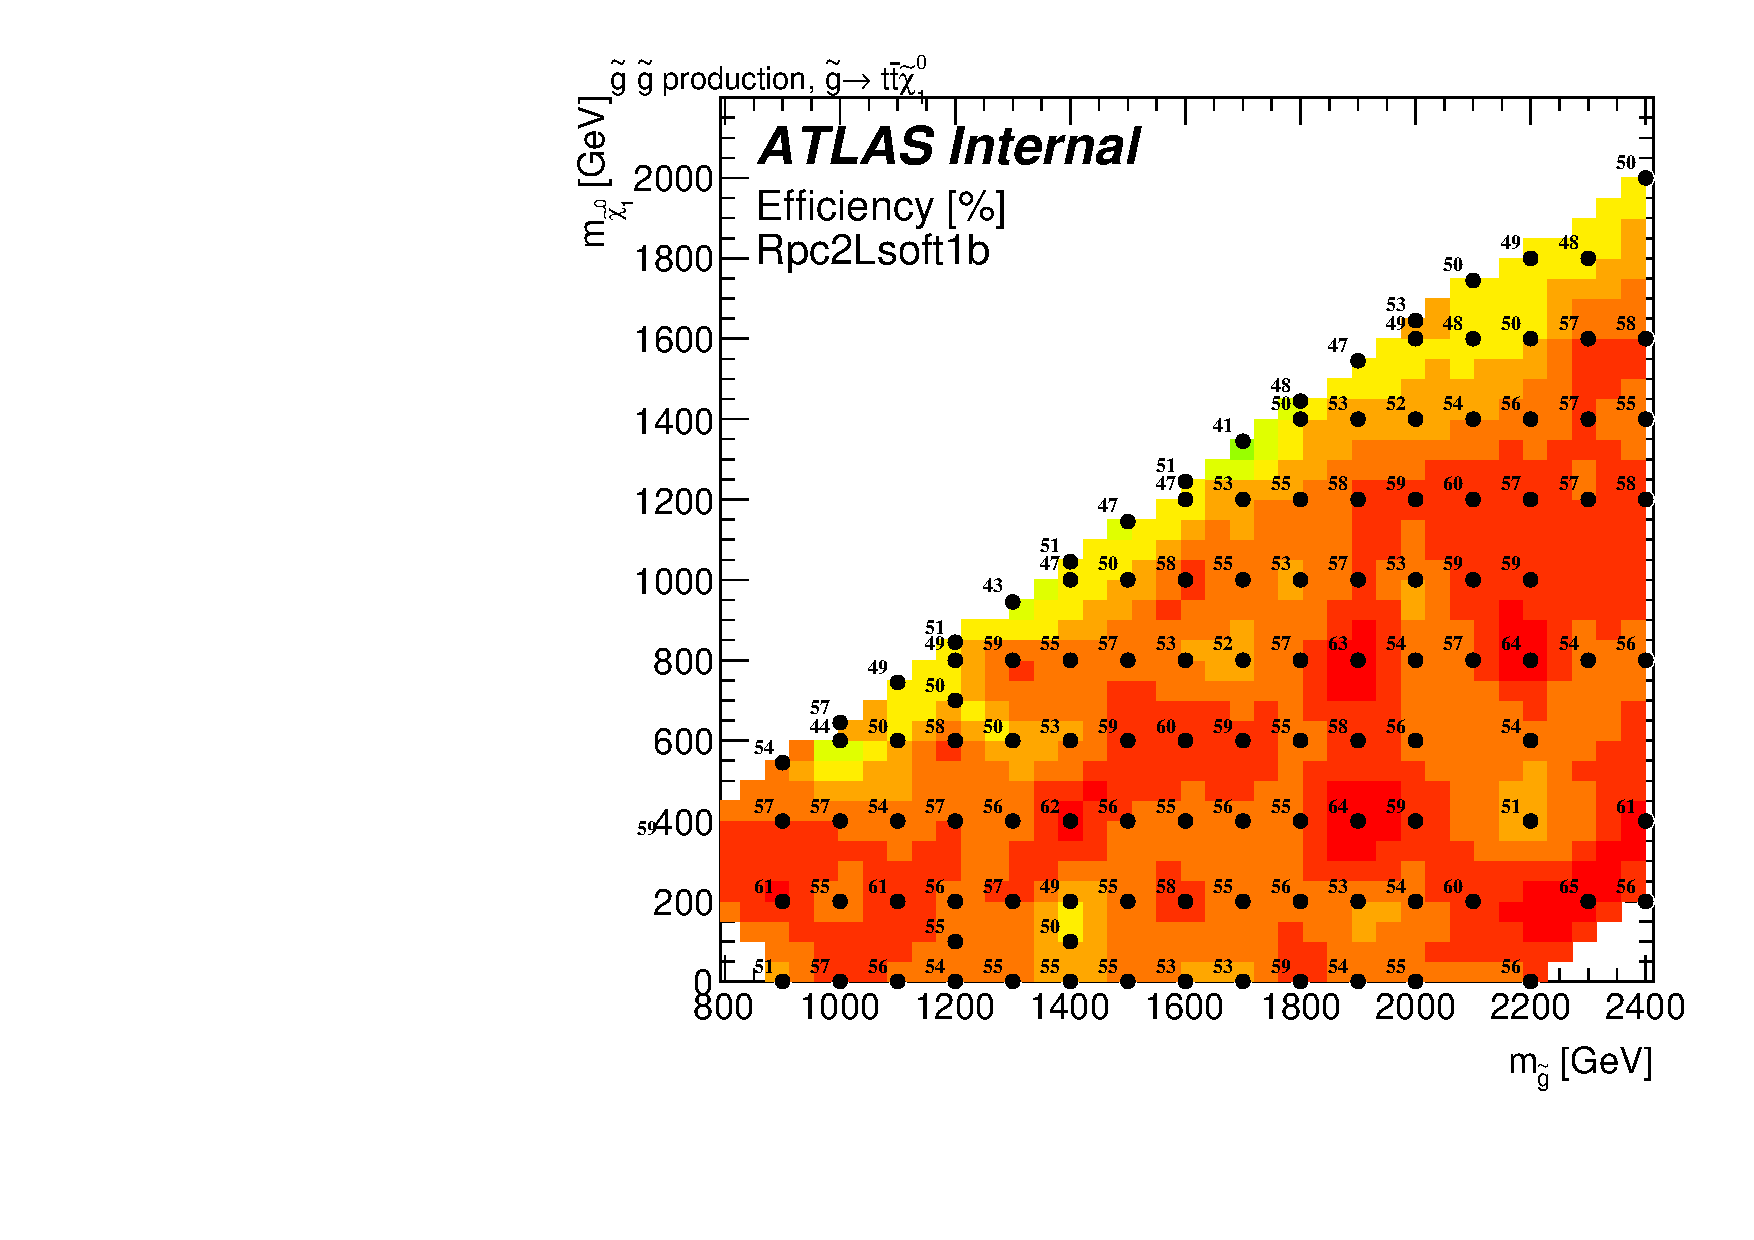
\includegraphics[width=\textwidth]{EffAcc/efficiency_GttRpc2Lsoft1b}\caption{Rpc2Lsoft1b efficiency}\end{subfigure}
\begin{subfigure}[t]{0.49\textwidth}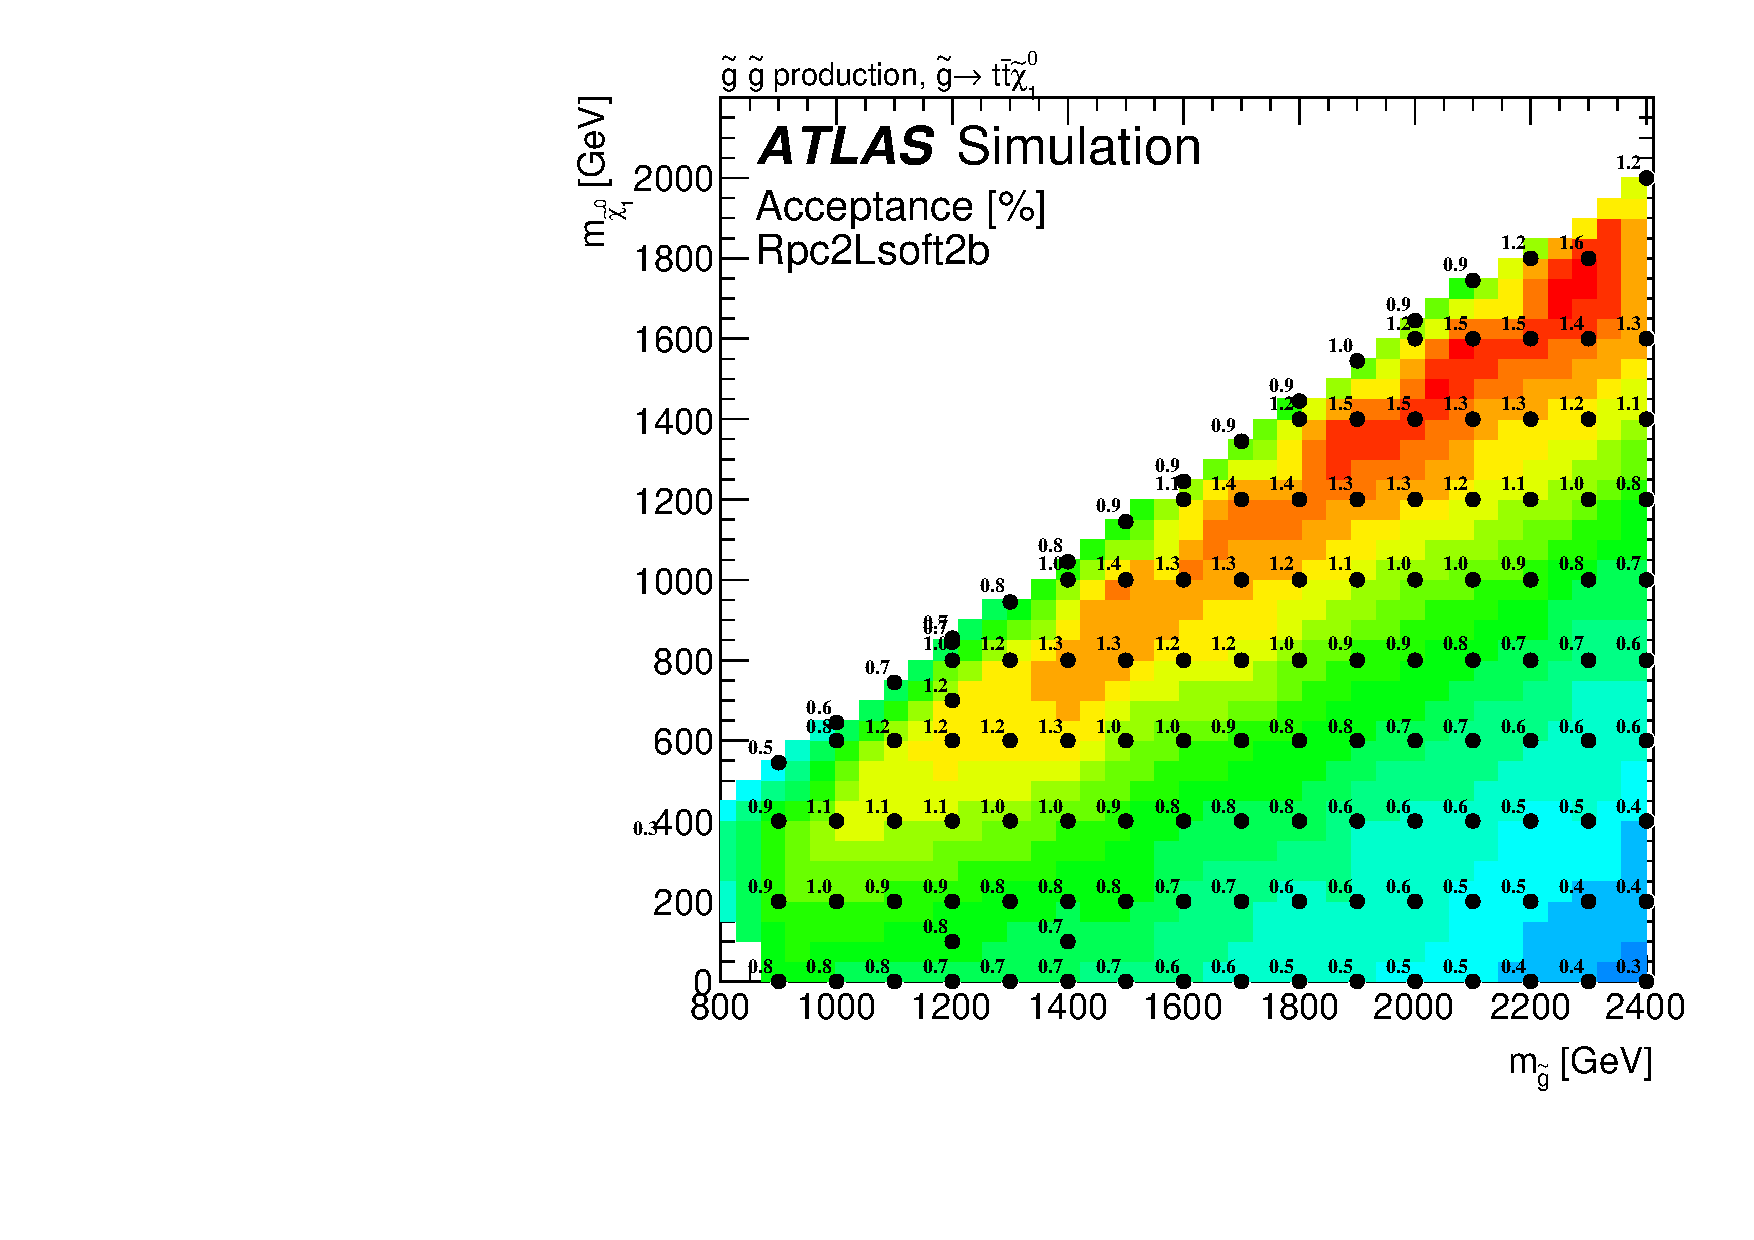
\includegraphics[width=\textwidth]{EffAcc/acceptance_GttRpc2Lsoft2b}\caption{Rpc2Lsoft2b acceptance}\end{subfigure}
\begin{subfigure}[t]{0.49\textwidth}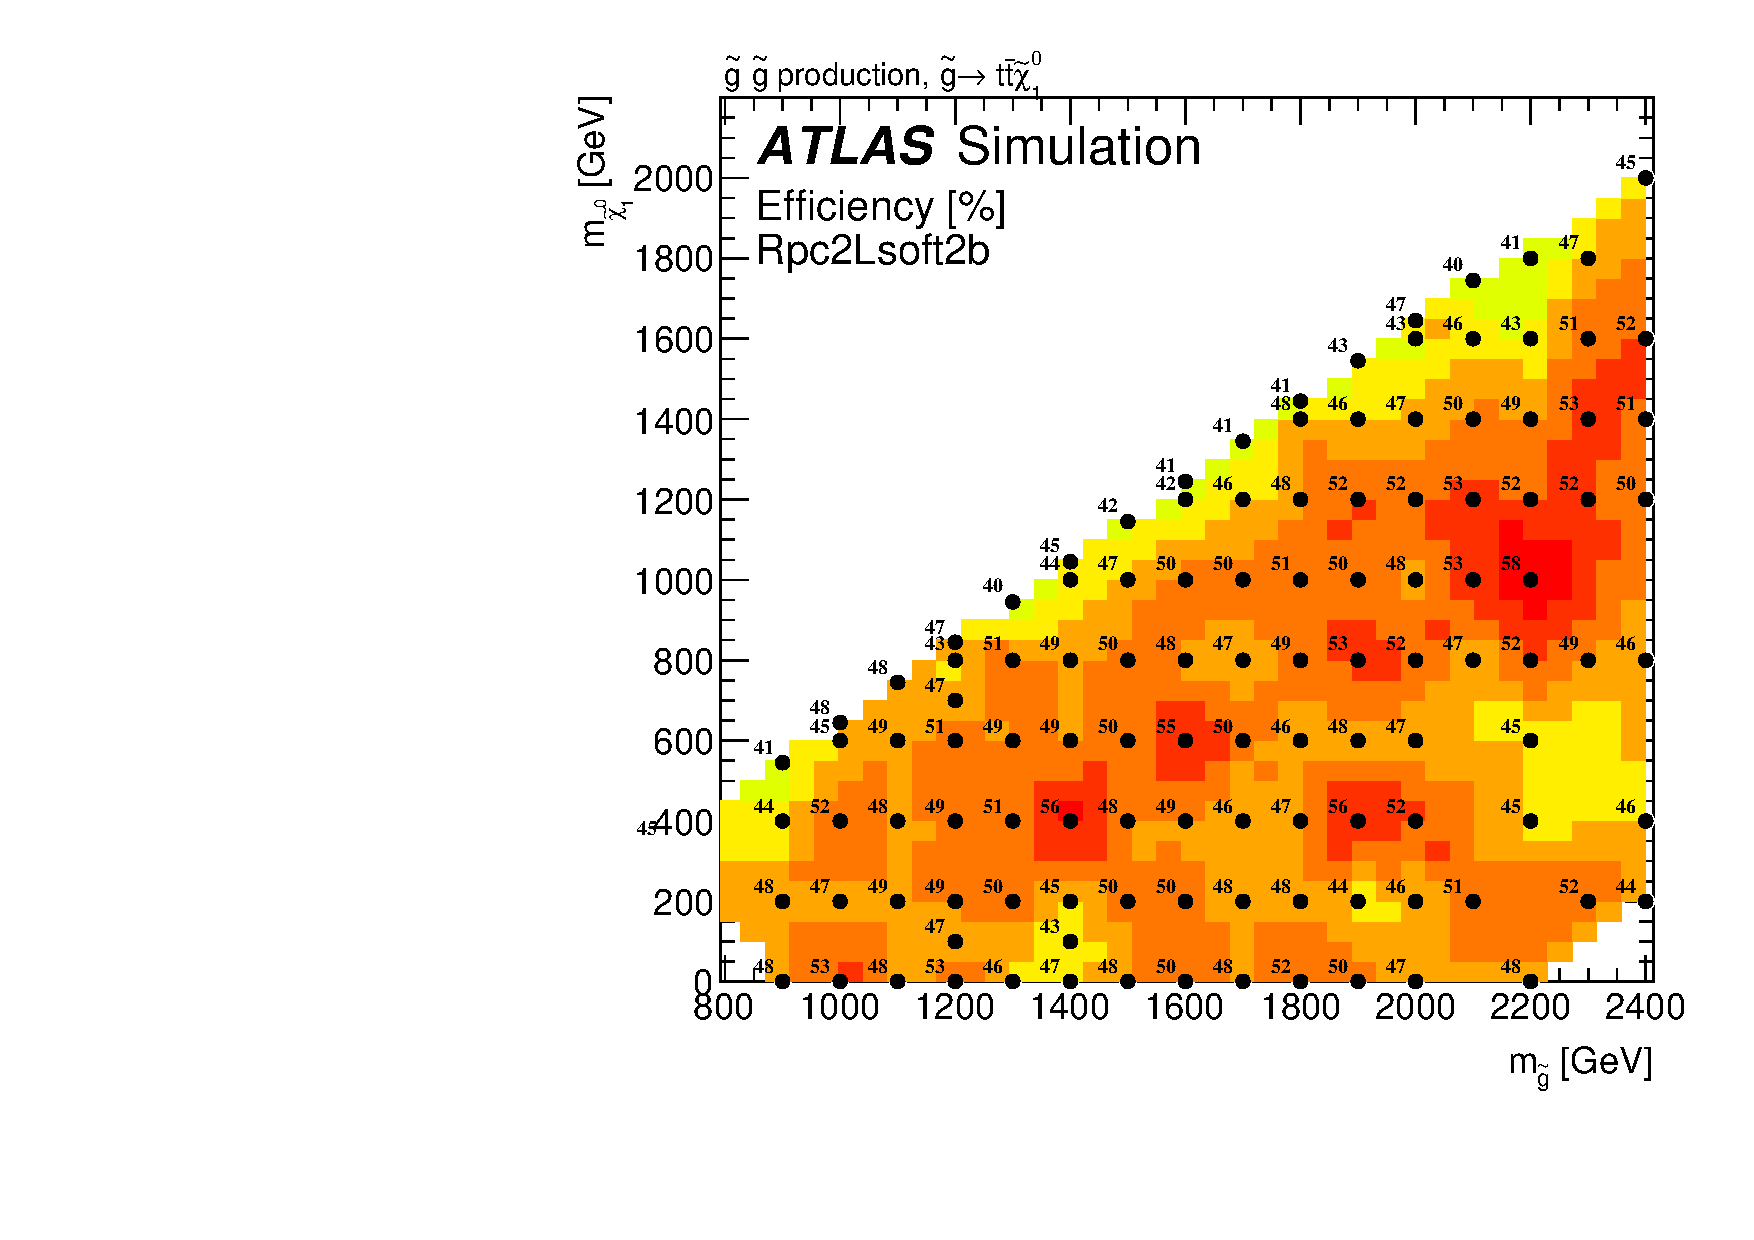
\includegraphics[width=\textwidth]{EffAcc/efficiency_GttRpc2Lsoft2b}\caption{Rpc2Lsoft2b efficiency}\end{subfigure}
\caption{Signal acceptance (a,c) and reconstruction efficiency (b,d) 
for simplified models of $\gluino\gluino$ production with $\gluino\to t\bar t\ninoone$ decays, 
in the signal regions Rpc2Lsoft1b (a,b) and Rpc2Lsoft2b (c,d).}
\end{figure}

\begin{figure}[htb!]
\centering
\begin{subfigure}[t]{0.49\textwidth}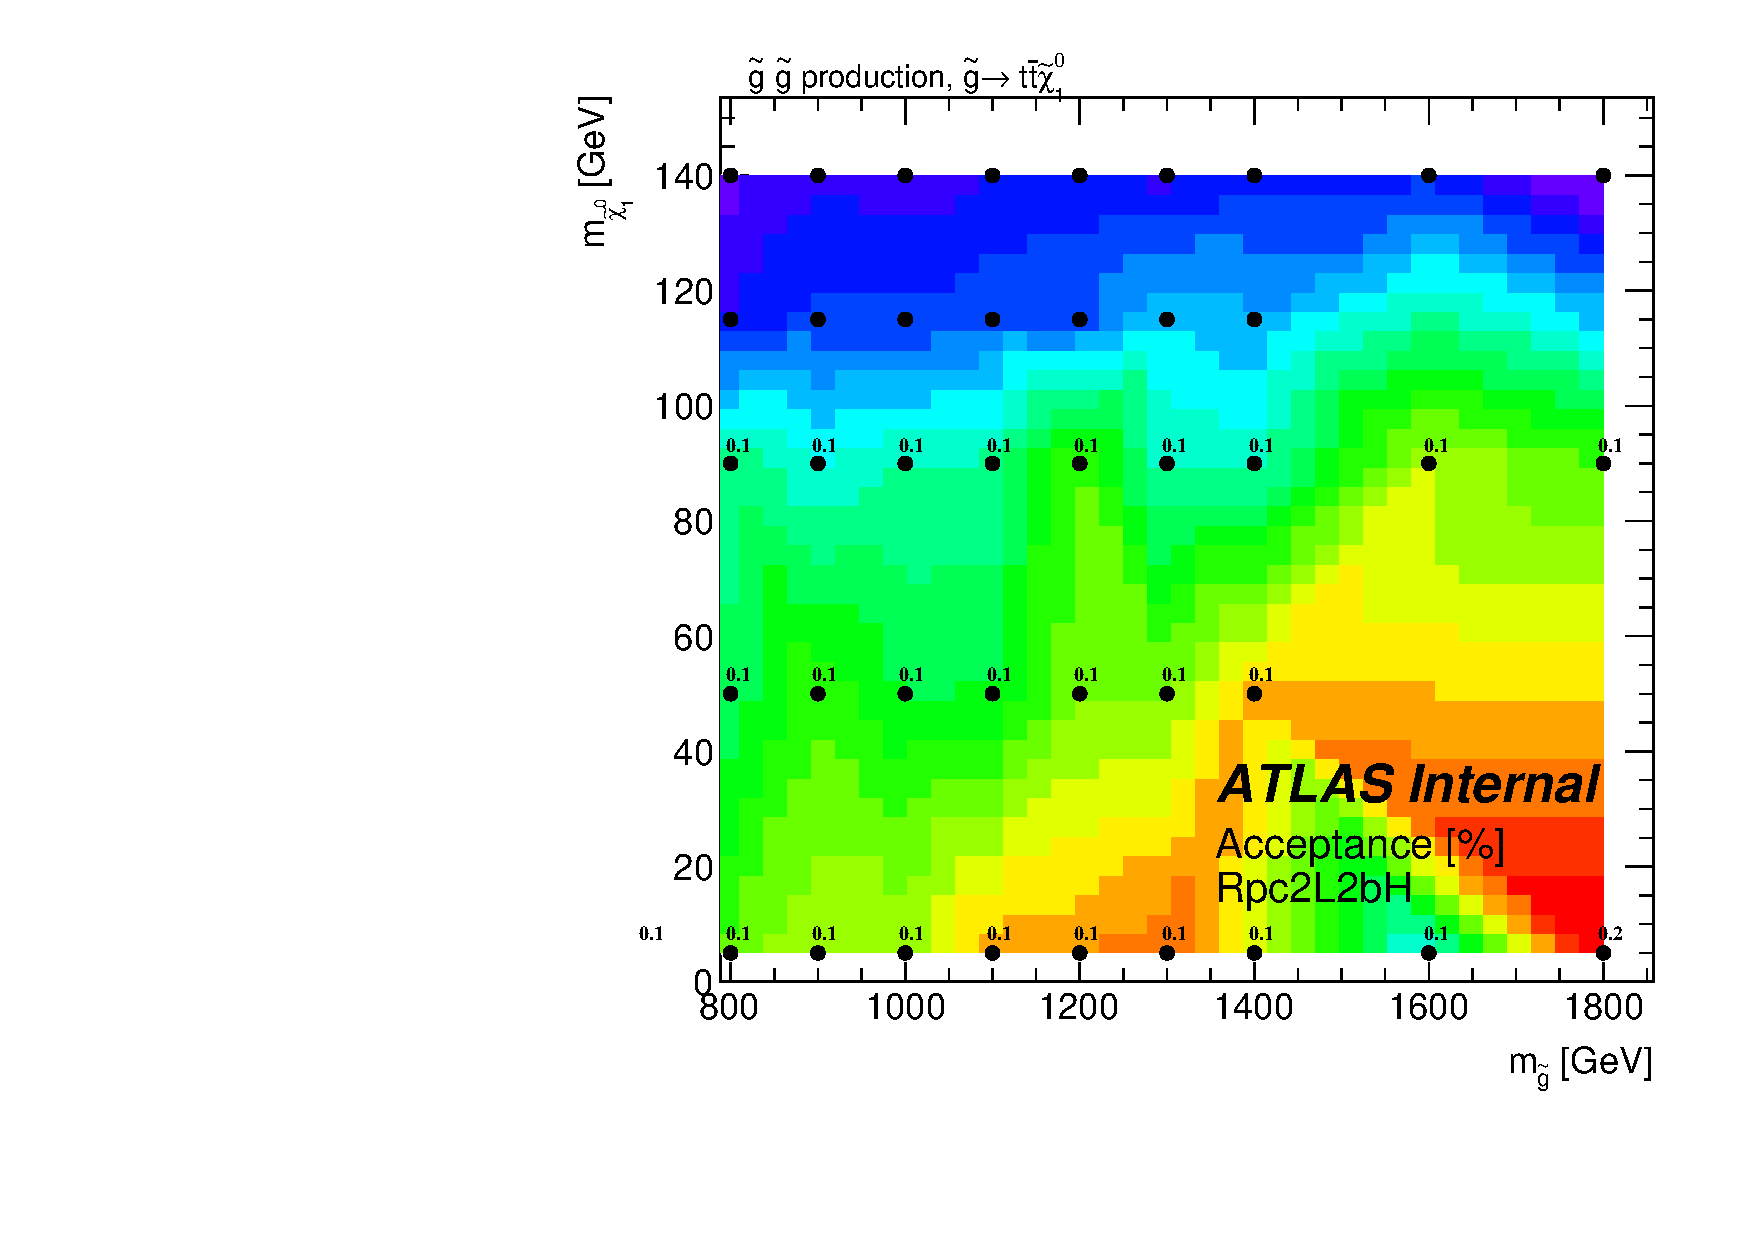
\includegraphics[width=\textwidth]{EffAcc/acceptance_ComprGttRpc2L2bH}\caption{Rpc2L2bH acceptance}\end{subfigure}
\begin{subfigure}[t]{0.49\textwidth}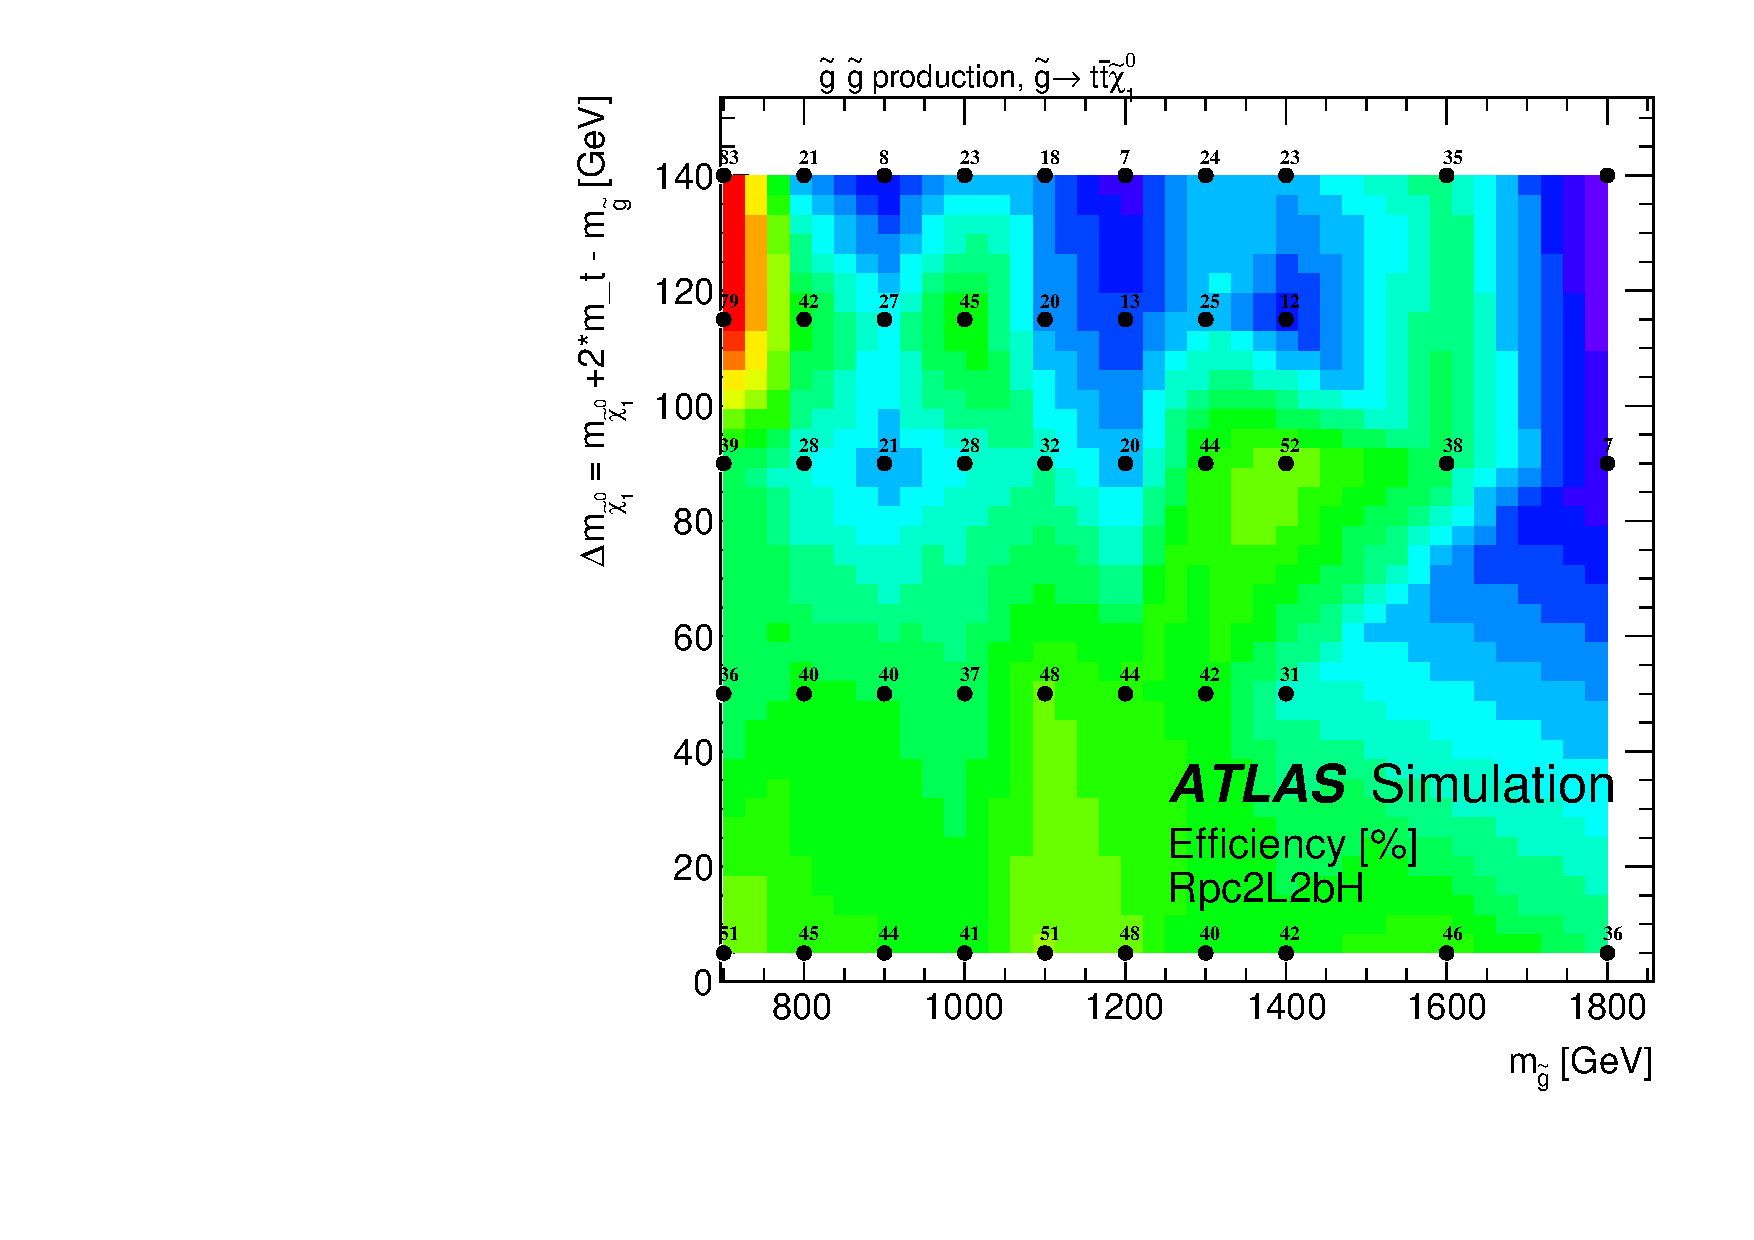
\includegraphics[width=\textwidth]{EffAcc/efficiency_ComprGttRpc2L2bH}\caption{Rpc2L2bH efficiency}\end{subfigure}
\begin{subfigure}[t]{0.49\textwidth}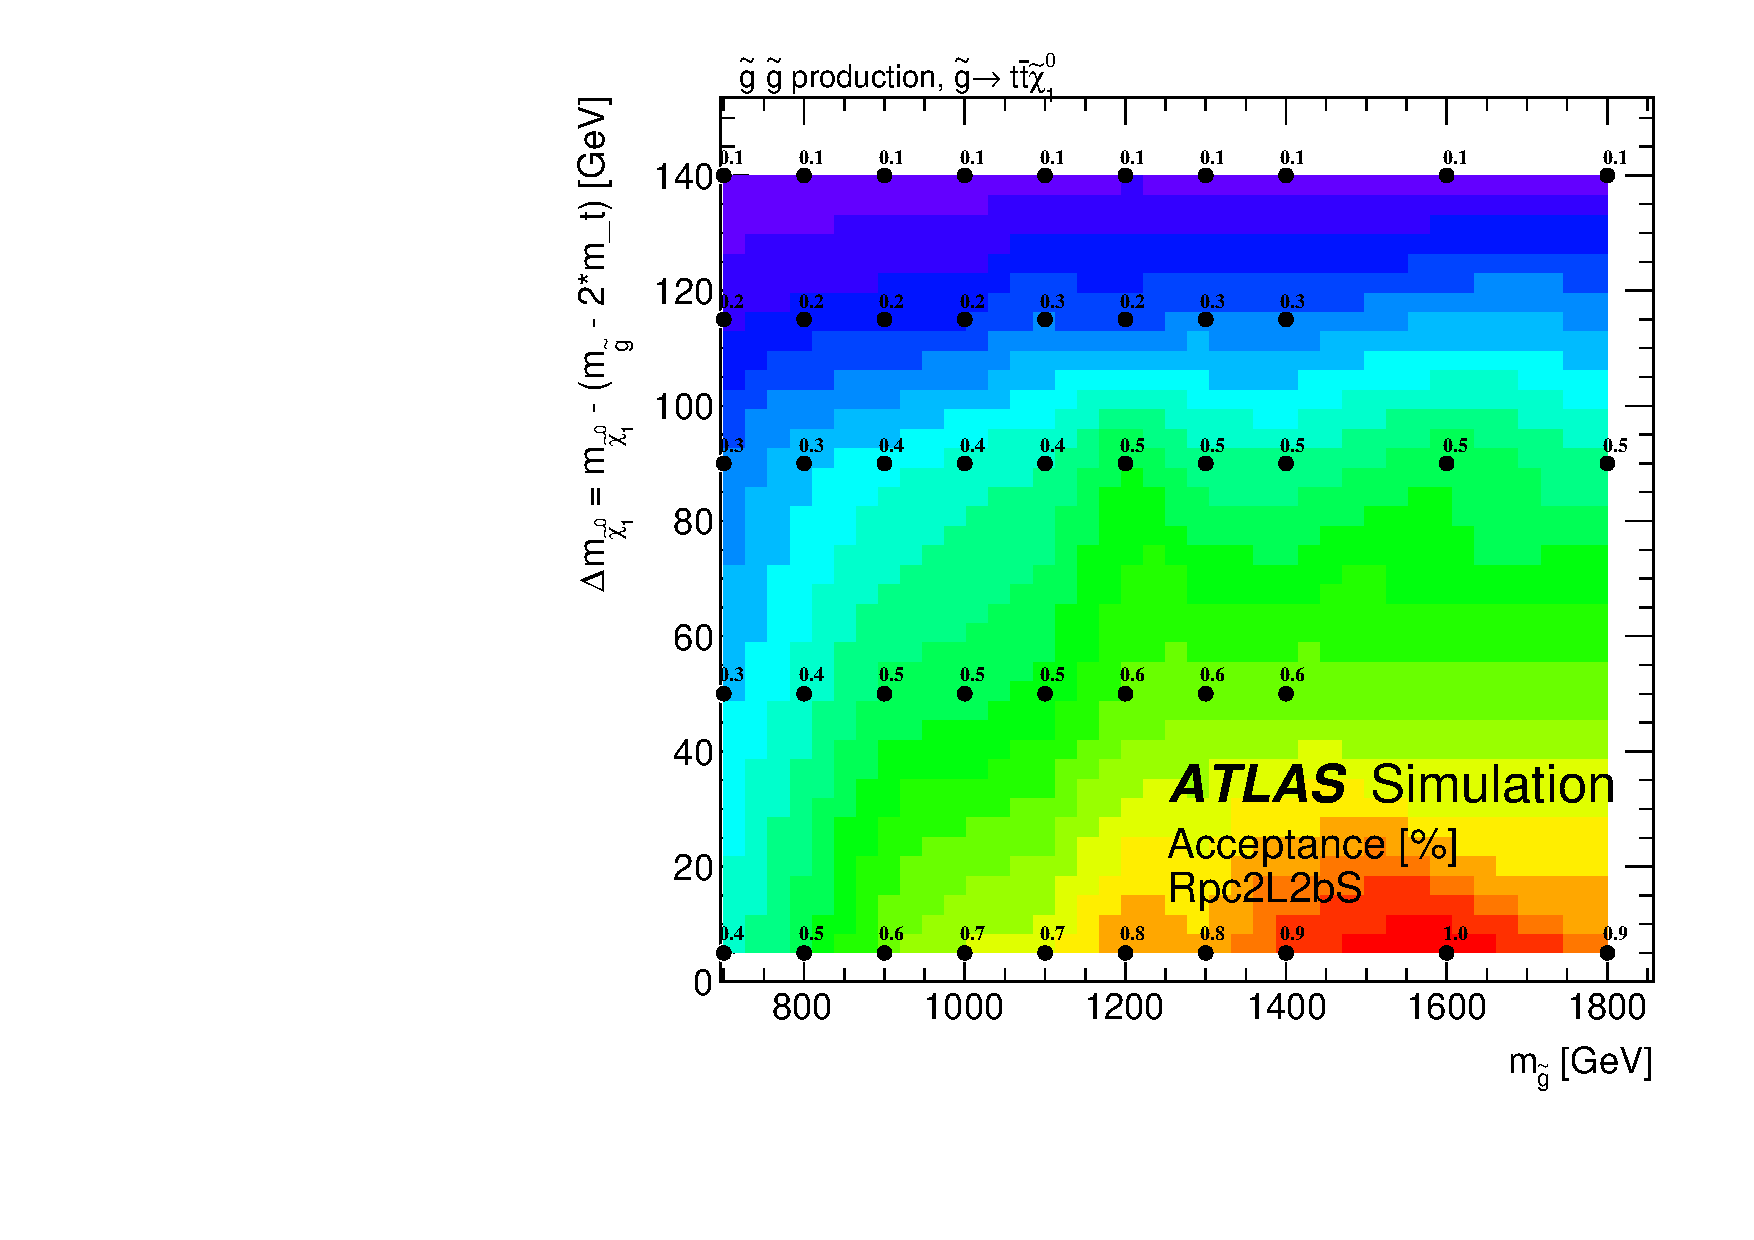
\includegraphics[width=\textwidth]{EffAcc/acceptance_ComprGttRpc2L2bS}\caption{Rpc2L2bS acceptance}\end{subfigure}
\begin{subfigure}[t]{0.49\textwidth}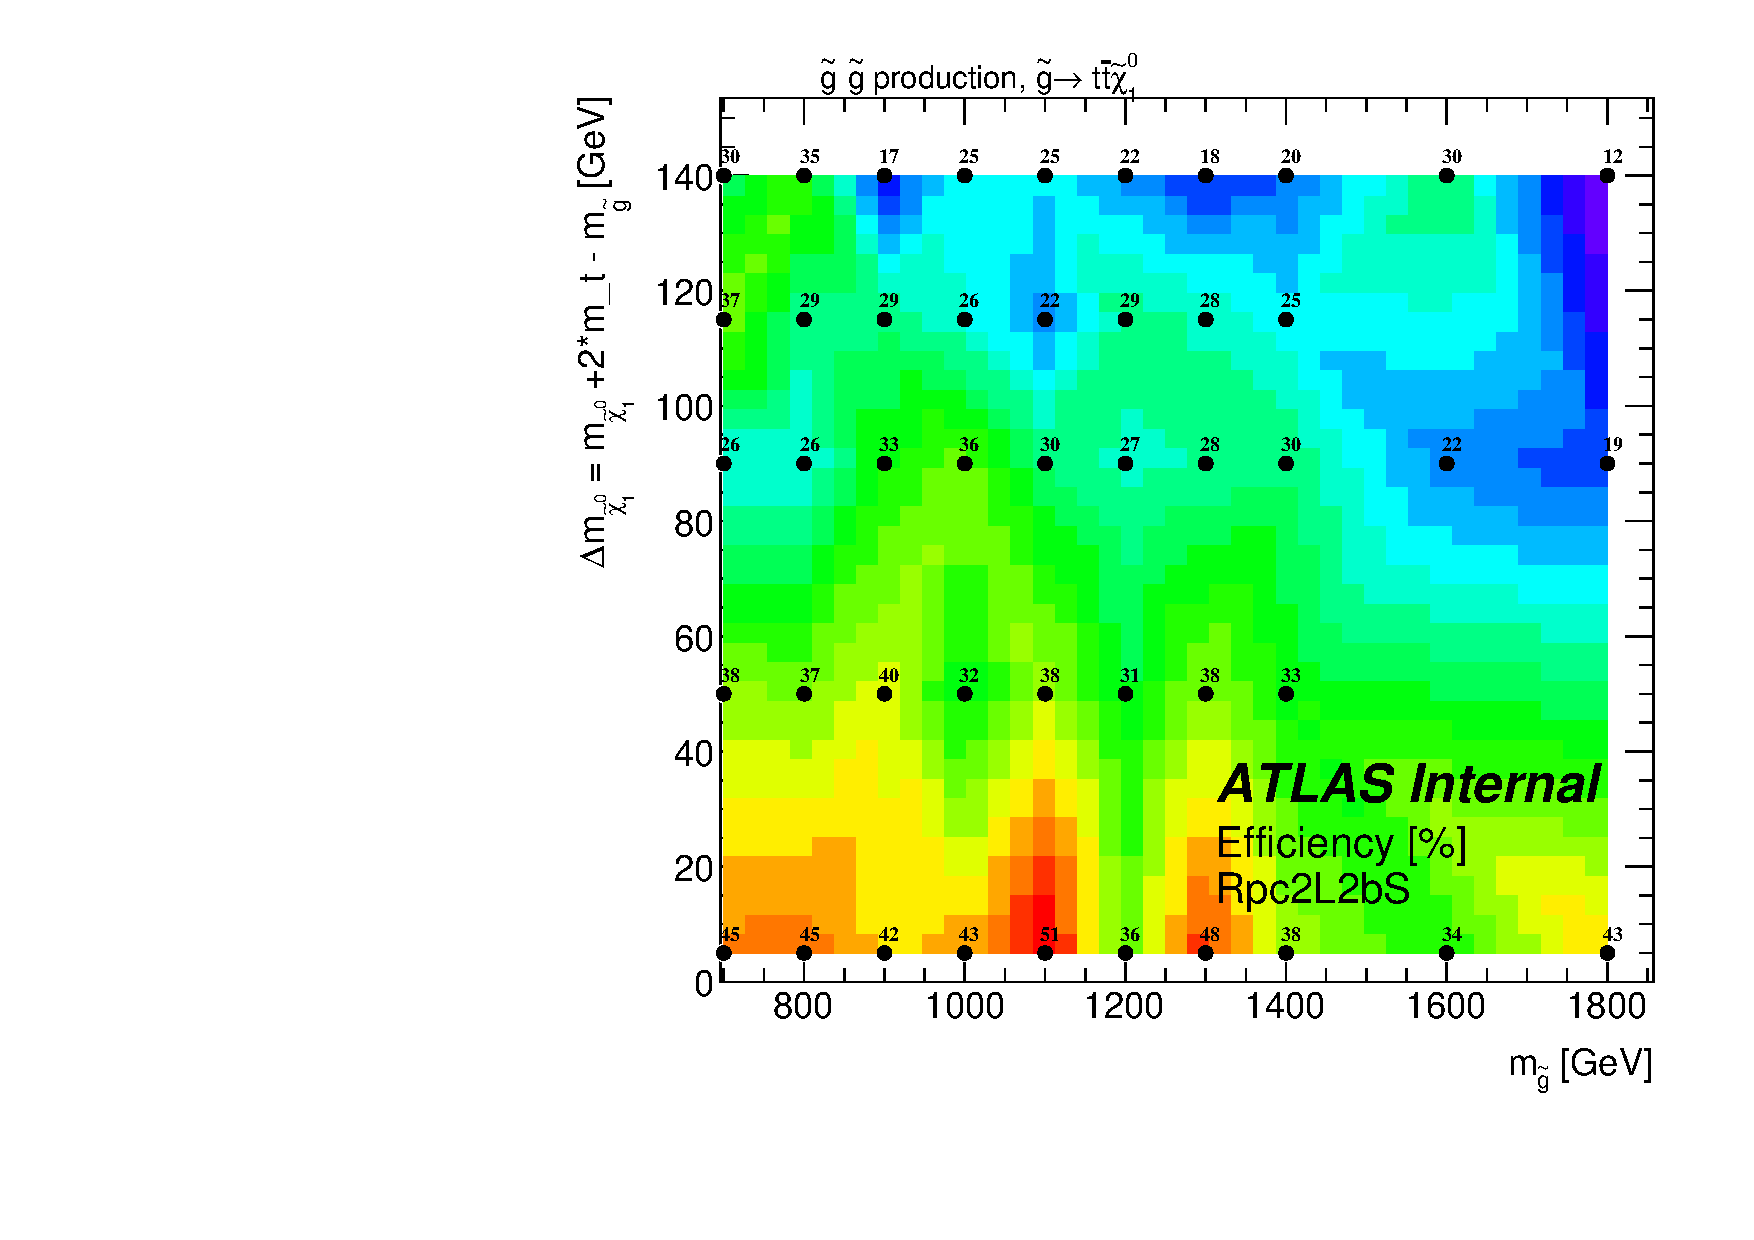
\includegraphics[width=\textwidth]{EffAcc/efficiency_ComprGttRpc2L2bS}\caption{Rpc2L2bS efficiency}\end{subfigure}
\caption{Signal acceptance (a,c) and reconstruction efficiency (b,d) 
for simplified models of $\gluino\gluino$ production with $\gluino\to tWb\ninoone$ decays (region with $\Delta m(\gluino,\ninoone)<2m_t$), 
in the signal regions Rpc2L2bH (a,b) and Rpc2L2bS (c,d).}
\end{figure}

\begin{figure}[htb!]
\centering
\begin{subfigure}[t]{0.49\textwidth}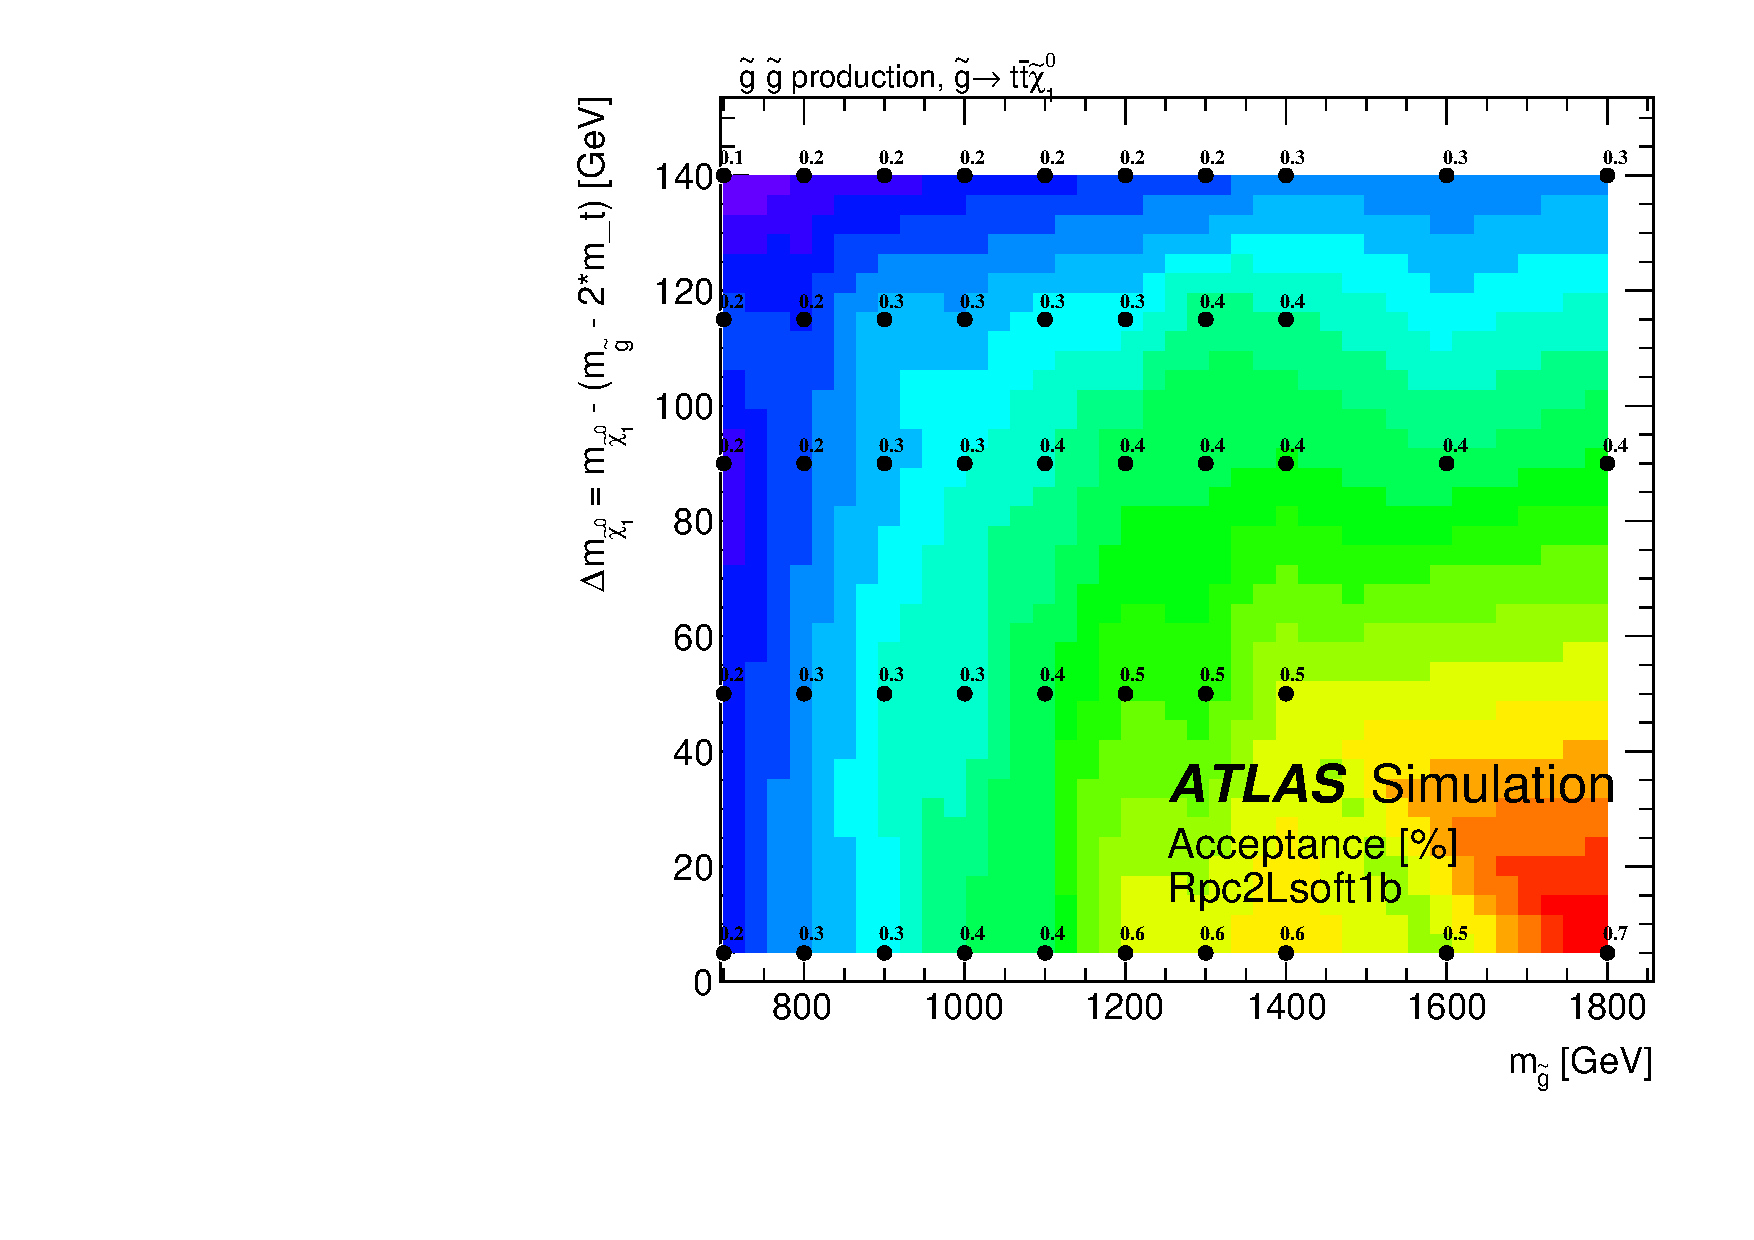
\includegraphics[width=\textwidth]{EffAcc/acceptance_ComprGttRpc2Lsoft1b}\caption{Rpc2Lsoft1b acceptance}\end{subfigure}
\begin{subfigure}[t]{0.49\textwidth}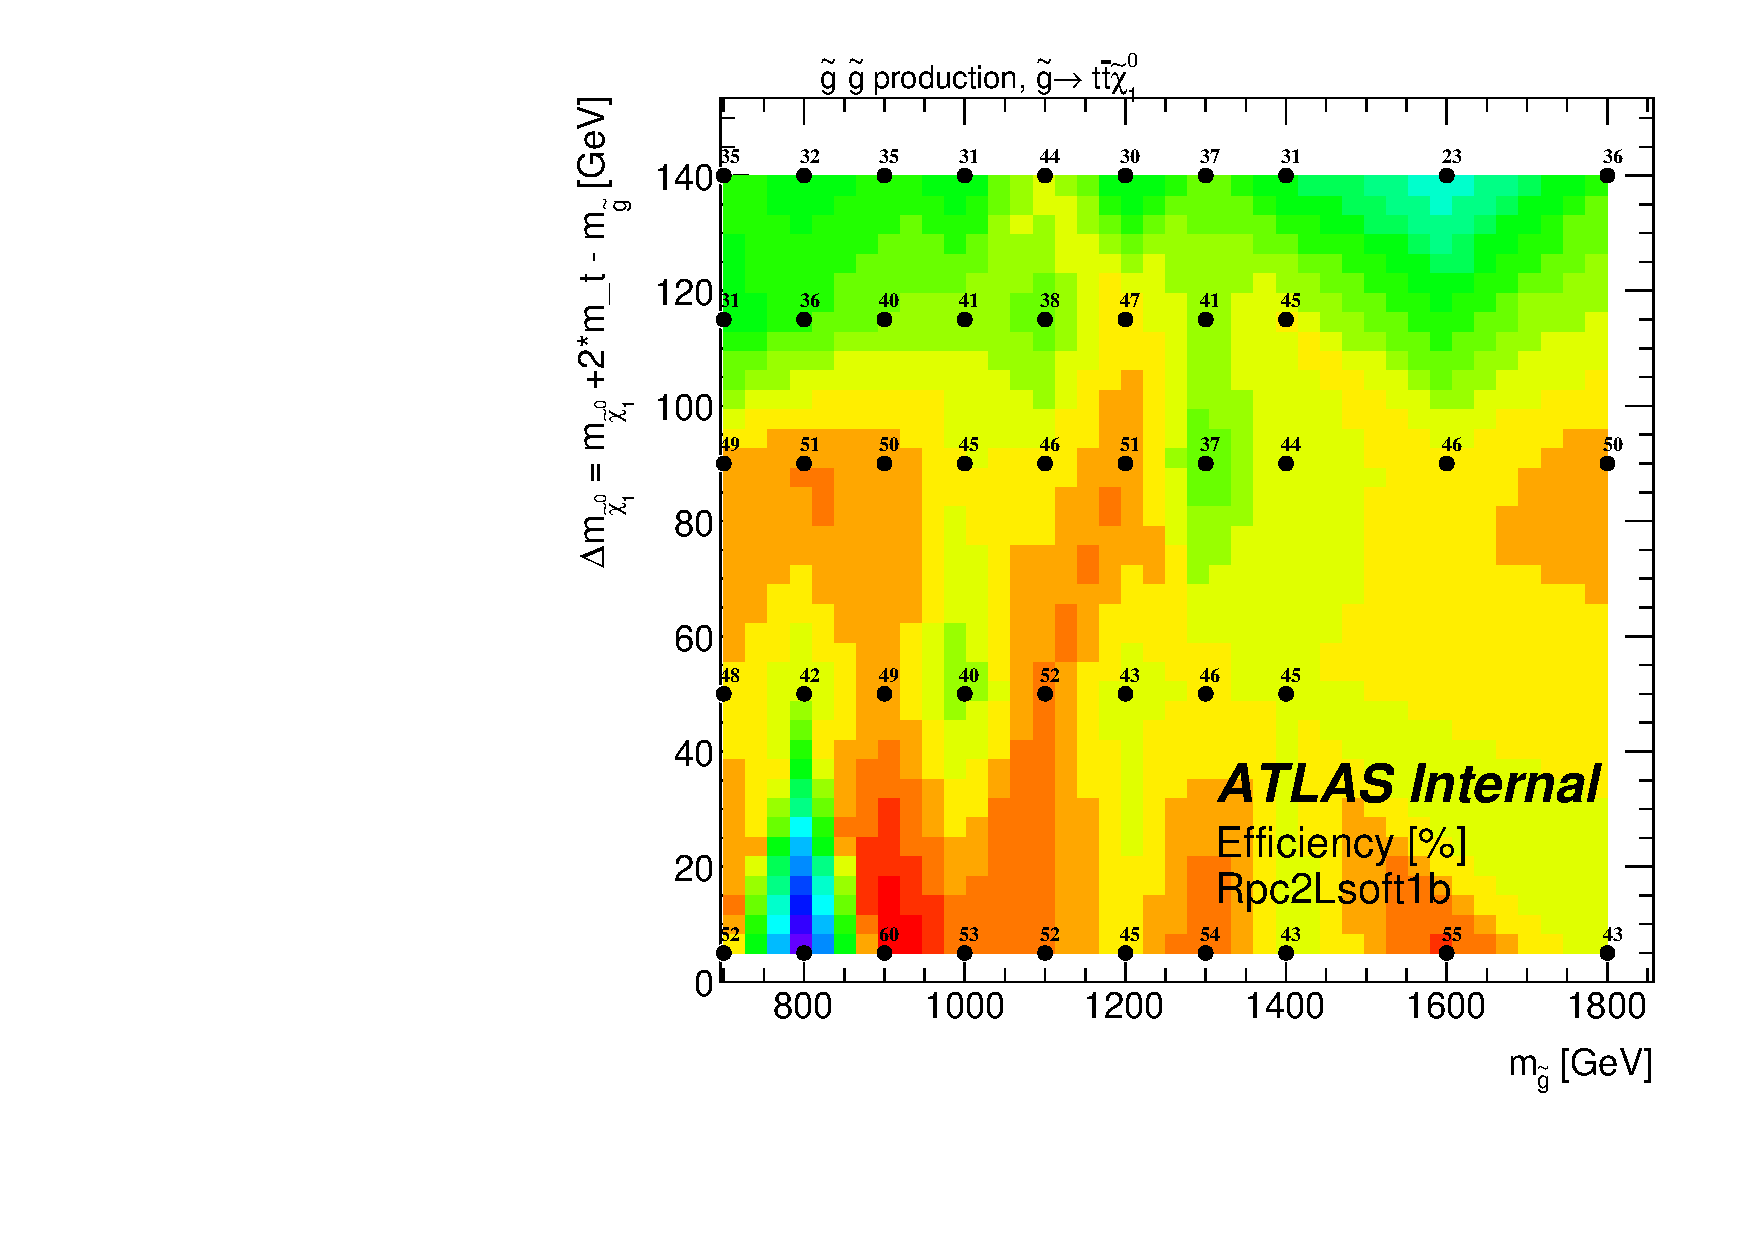
\includegraphics[width=\textwidth]{EffAcc/efficiency_ComprGttRpc2Lsoft1b}\caption{Rpc2Lsoft1b efficiency}\end{subfigure}
\begin{subfigure}[t]{0.49\textwidth}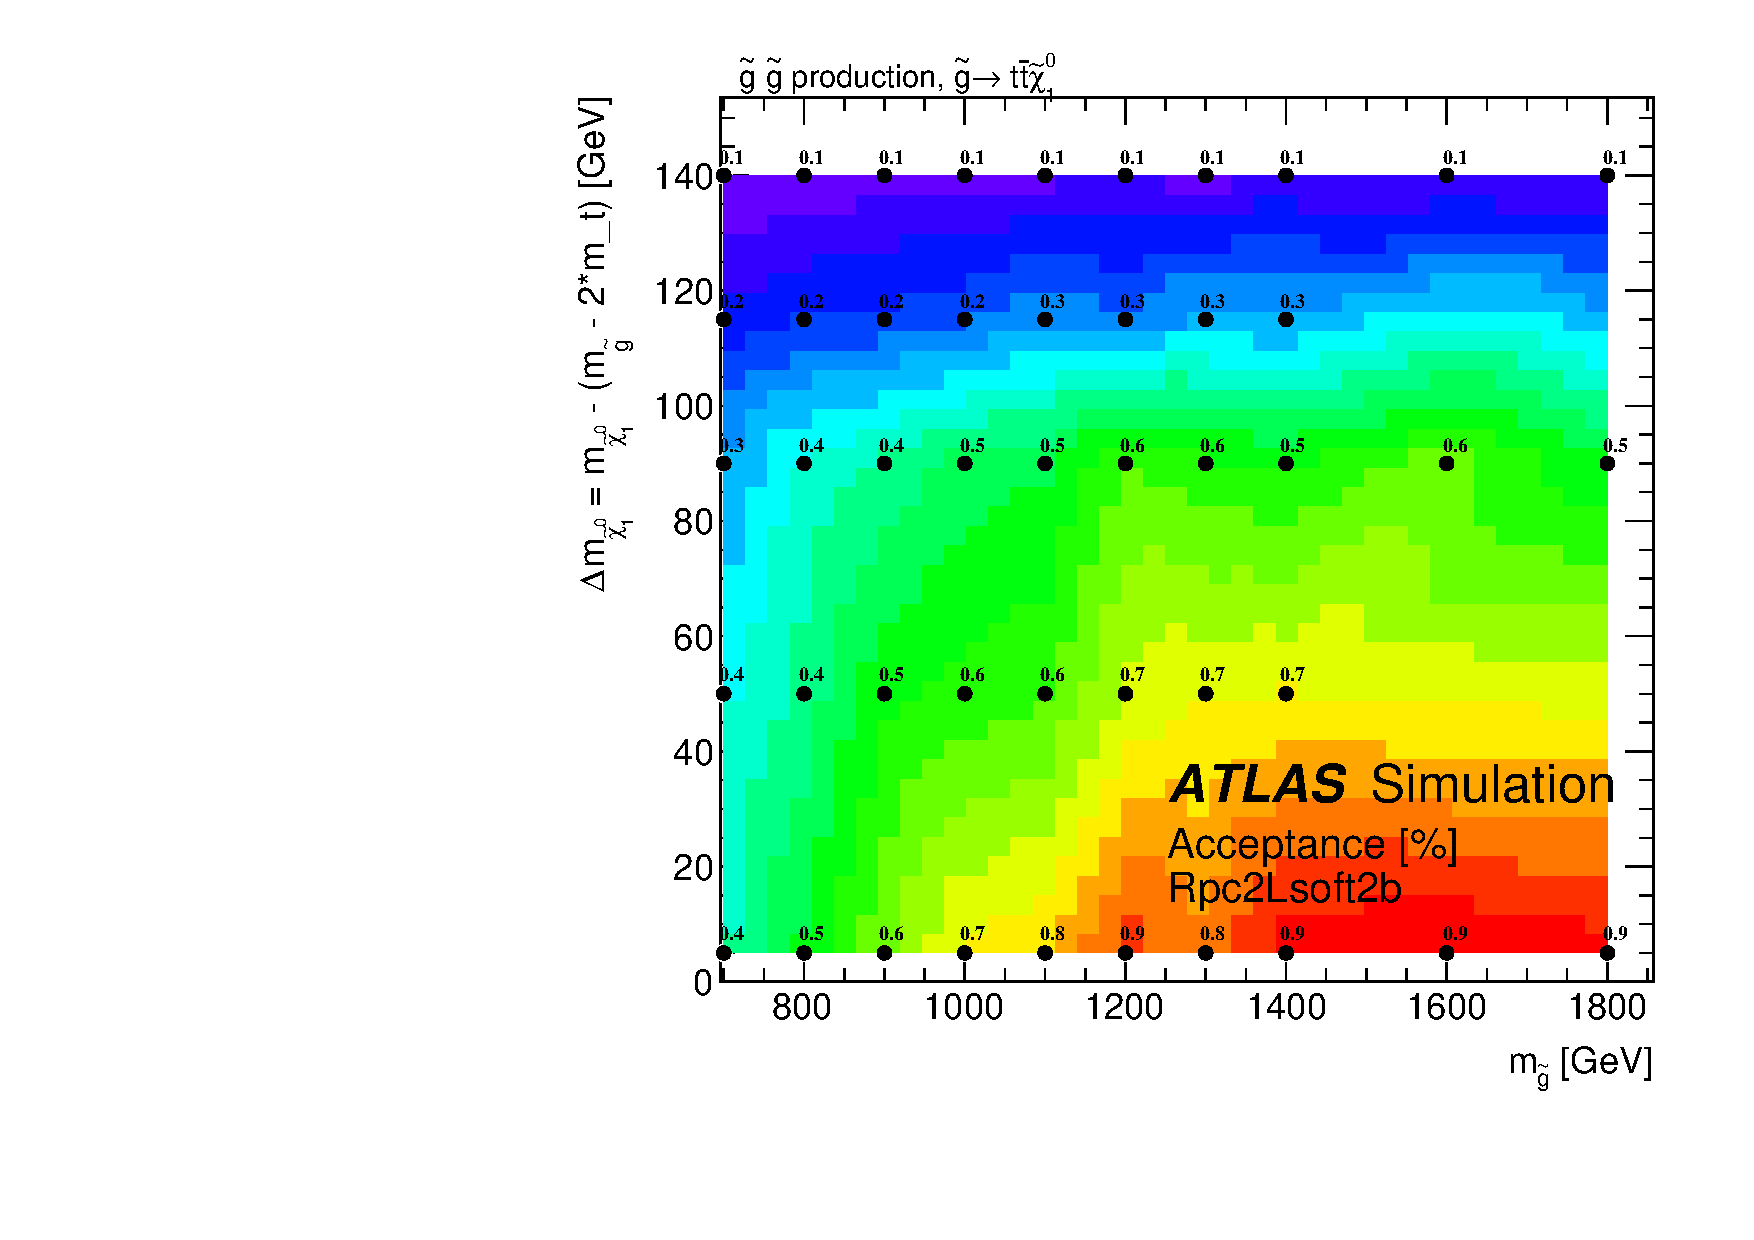
\includegraphics[width=\textwidth]{EffAcc/acceptance_ComprGttRpc2Lsoft2b}\caption{Rpc2Lsoft2b acceptance}\end{subfigure}
\begin{subfigure}[t]{0.49\textwidth}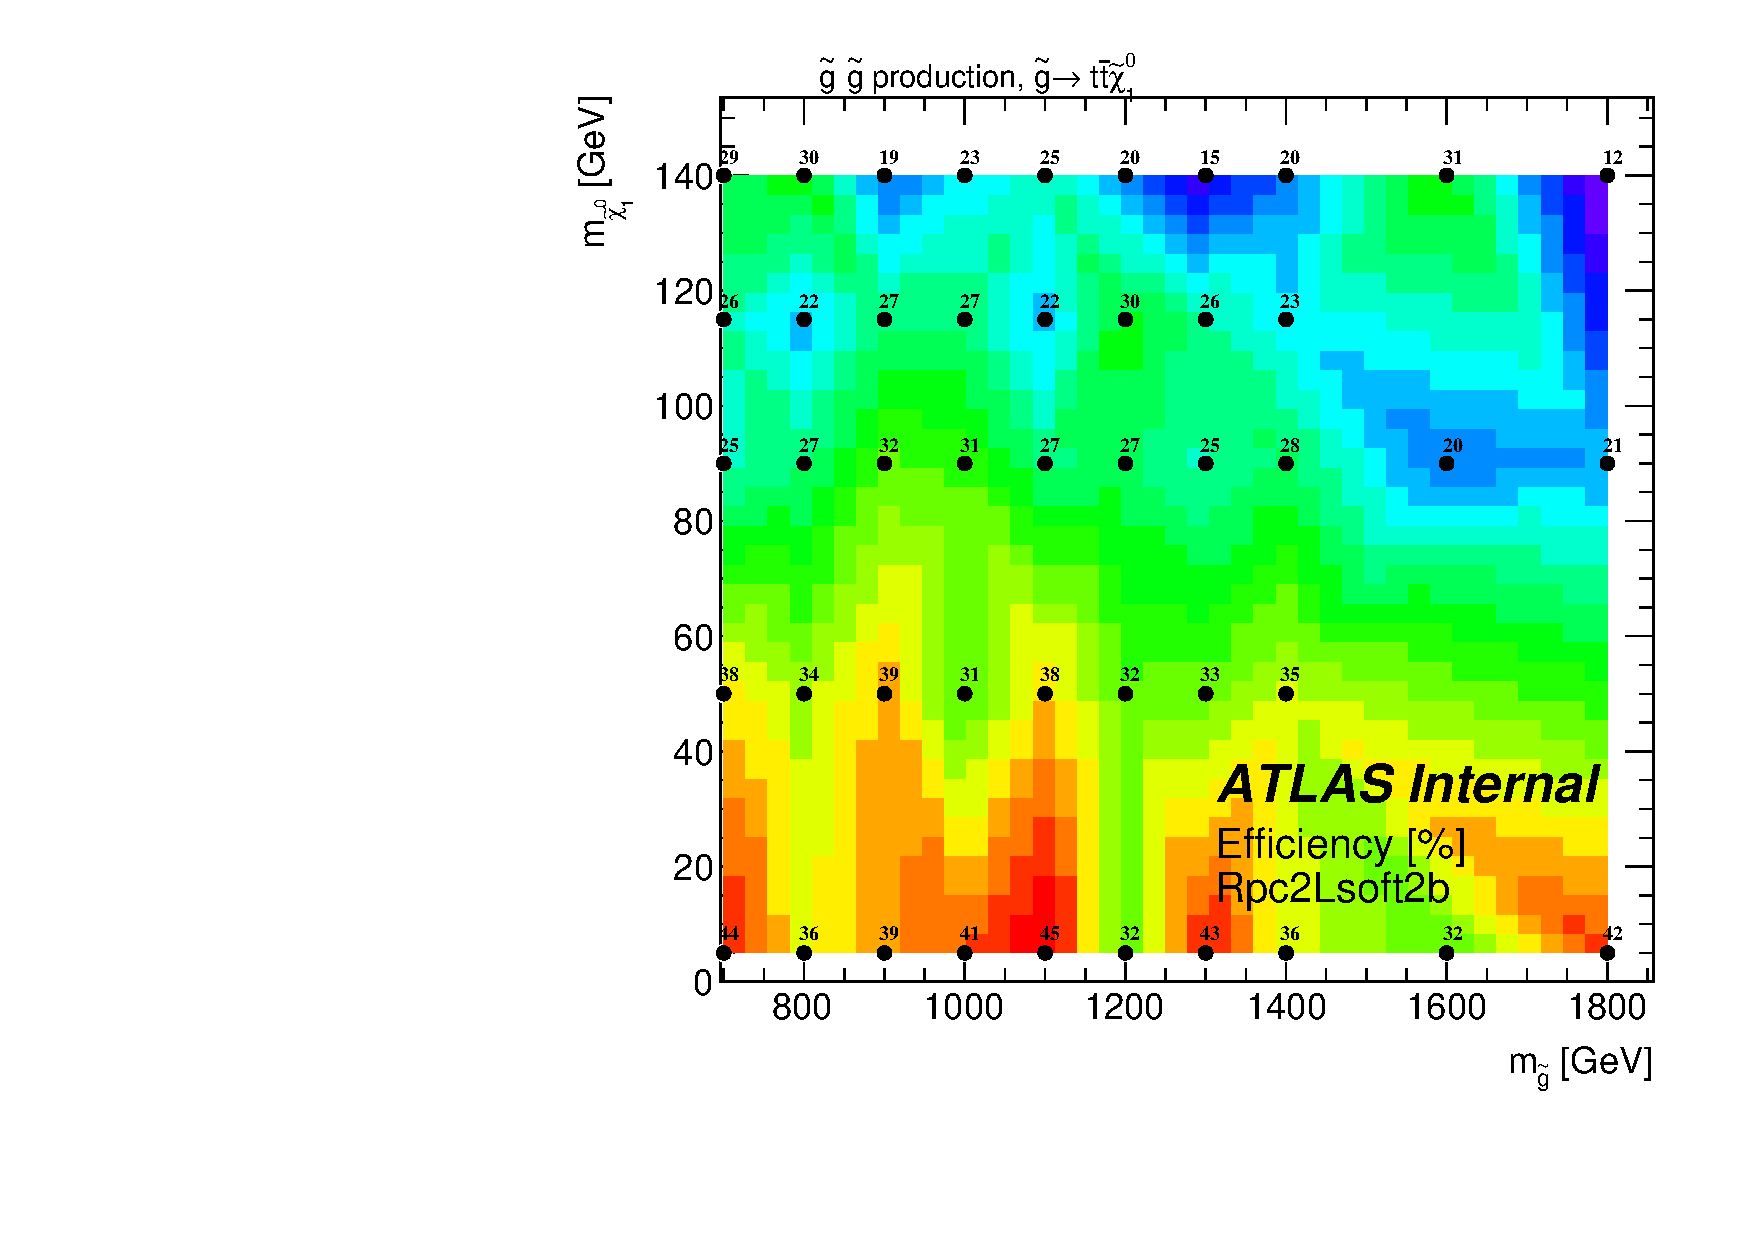
\includegraphics[width=\textwidth]{EffAcc/efficiency_ComprGttRpc2Lsoft2b}\caption{Rpc2Lsoft2b efficiency}\end{subfigure}
\caption{Signal acceptance (a,c) and reconstruction efficiency (b,d) 
for simplified models of $\gluino\gluino$ production with $\gluino\to tWb\ninoone$ decays (region with $\Delta m(\gluino,\ninoone)<2m_t$), 
in the signal regions Rpc2Lsoft1b (a,b) and Rpc2Lsoft2b (c,d).}
\end{figure}

\begin{figure}[htb!]
\centering
\begin{subfigure}[t]{0.49\textwidth}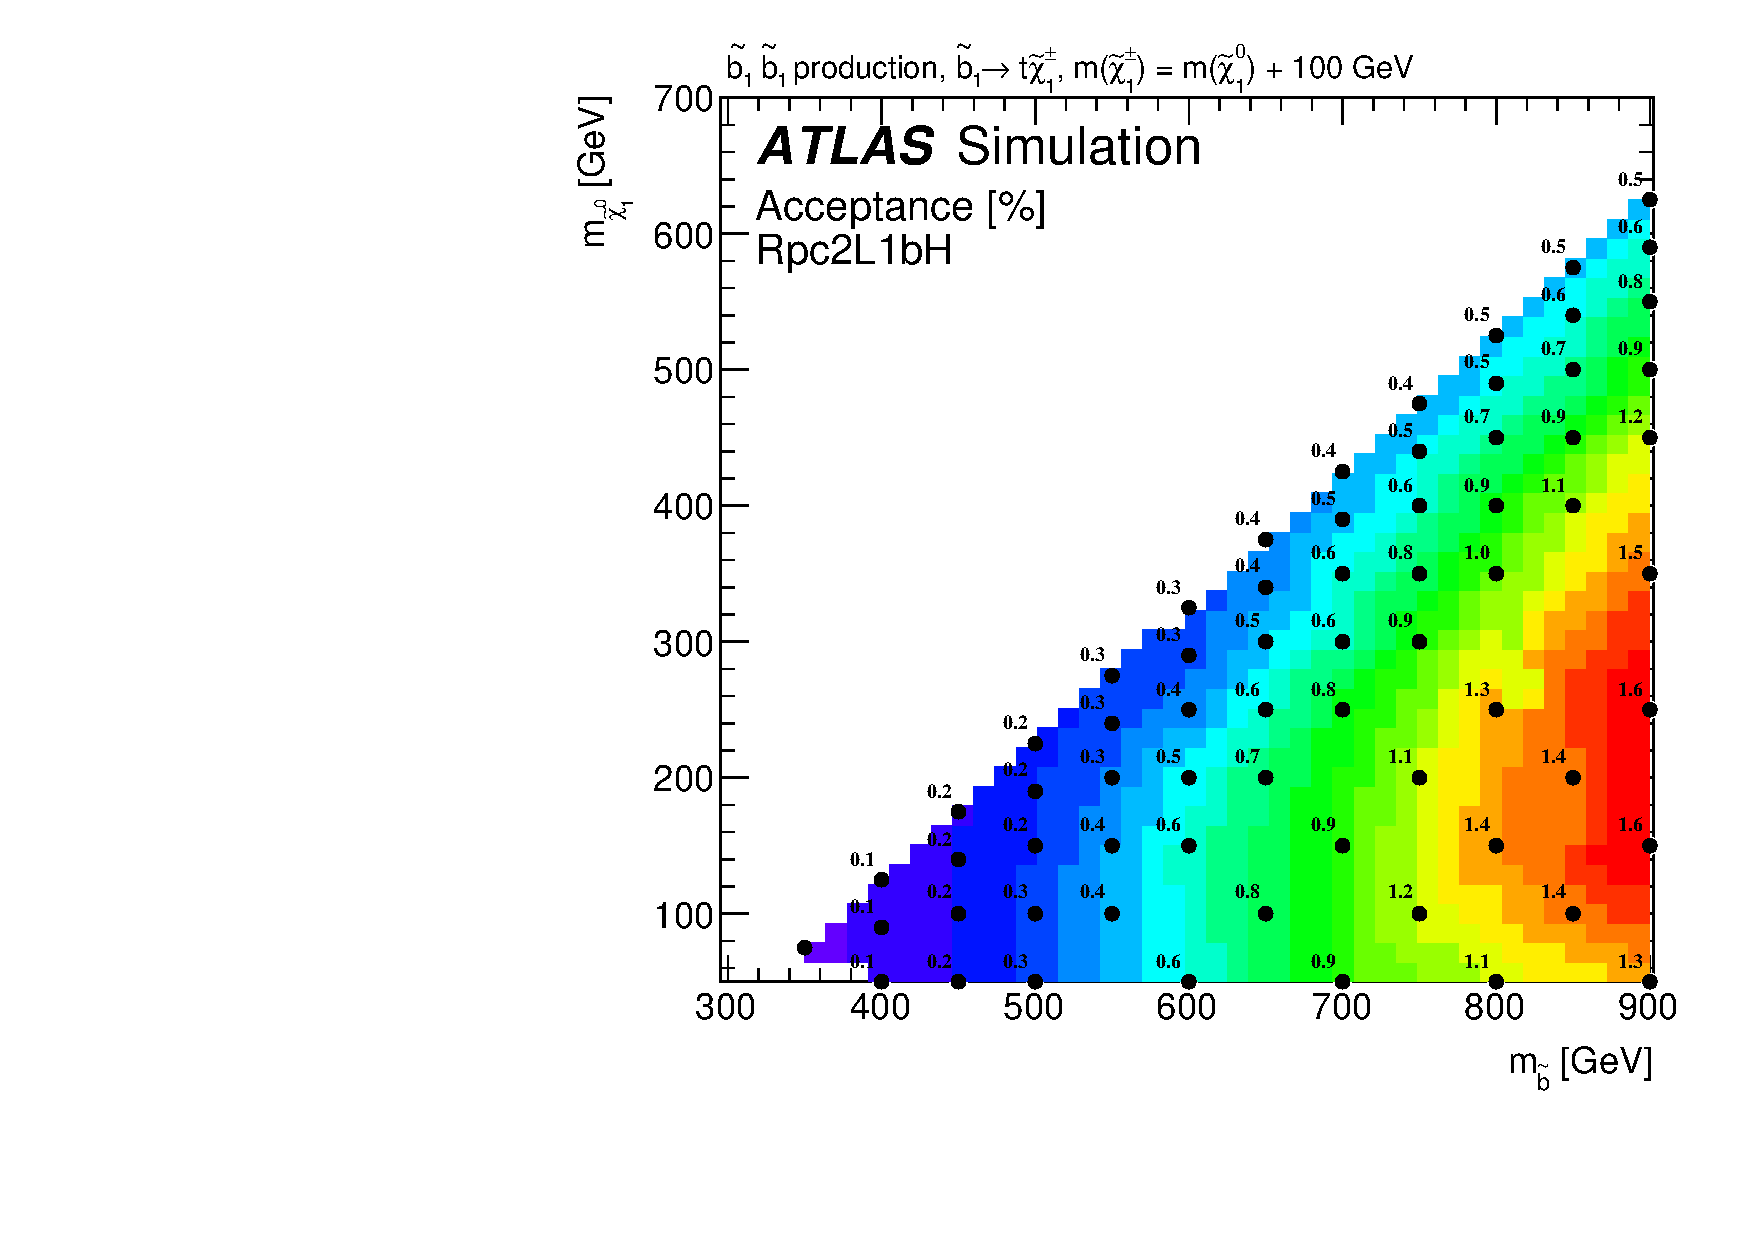
\includegraphics[width=\textwidth]{EffAcc/acceptance_BttRpc2L1bH}\caption{Rpc2L1bH acceptance}\end{subfigure}
\begin{subfigure}[t]{0.49\textwidth}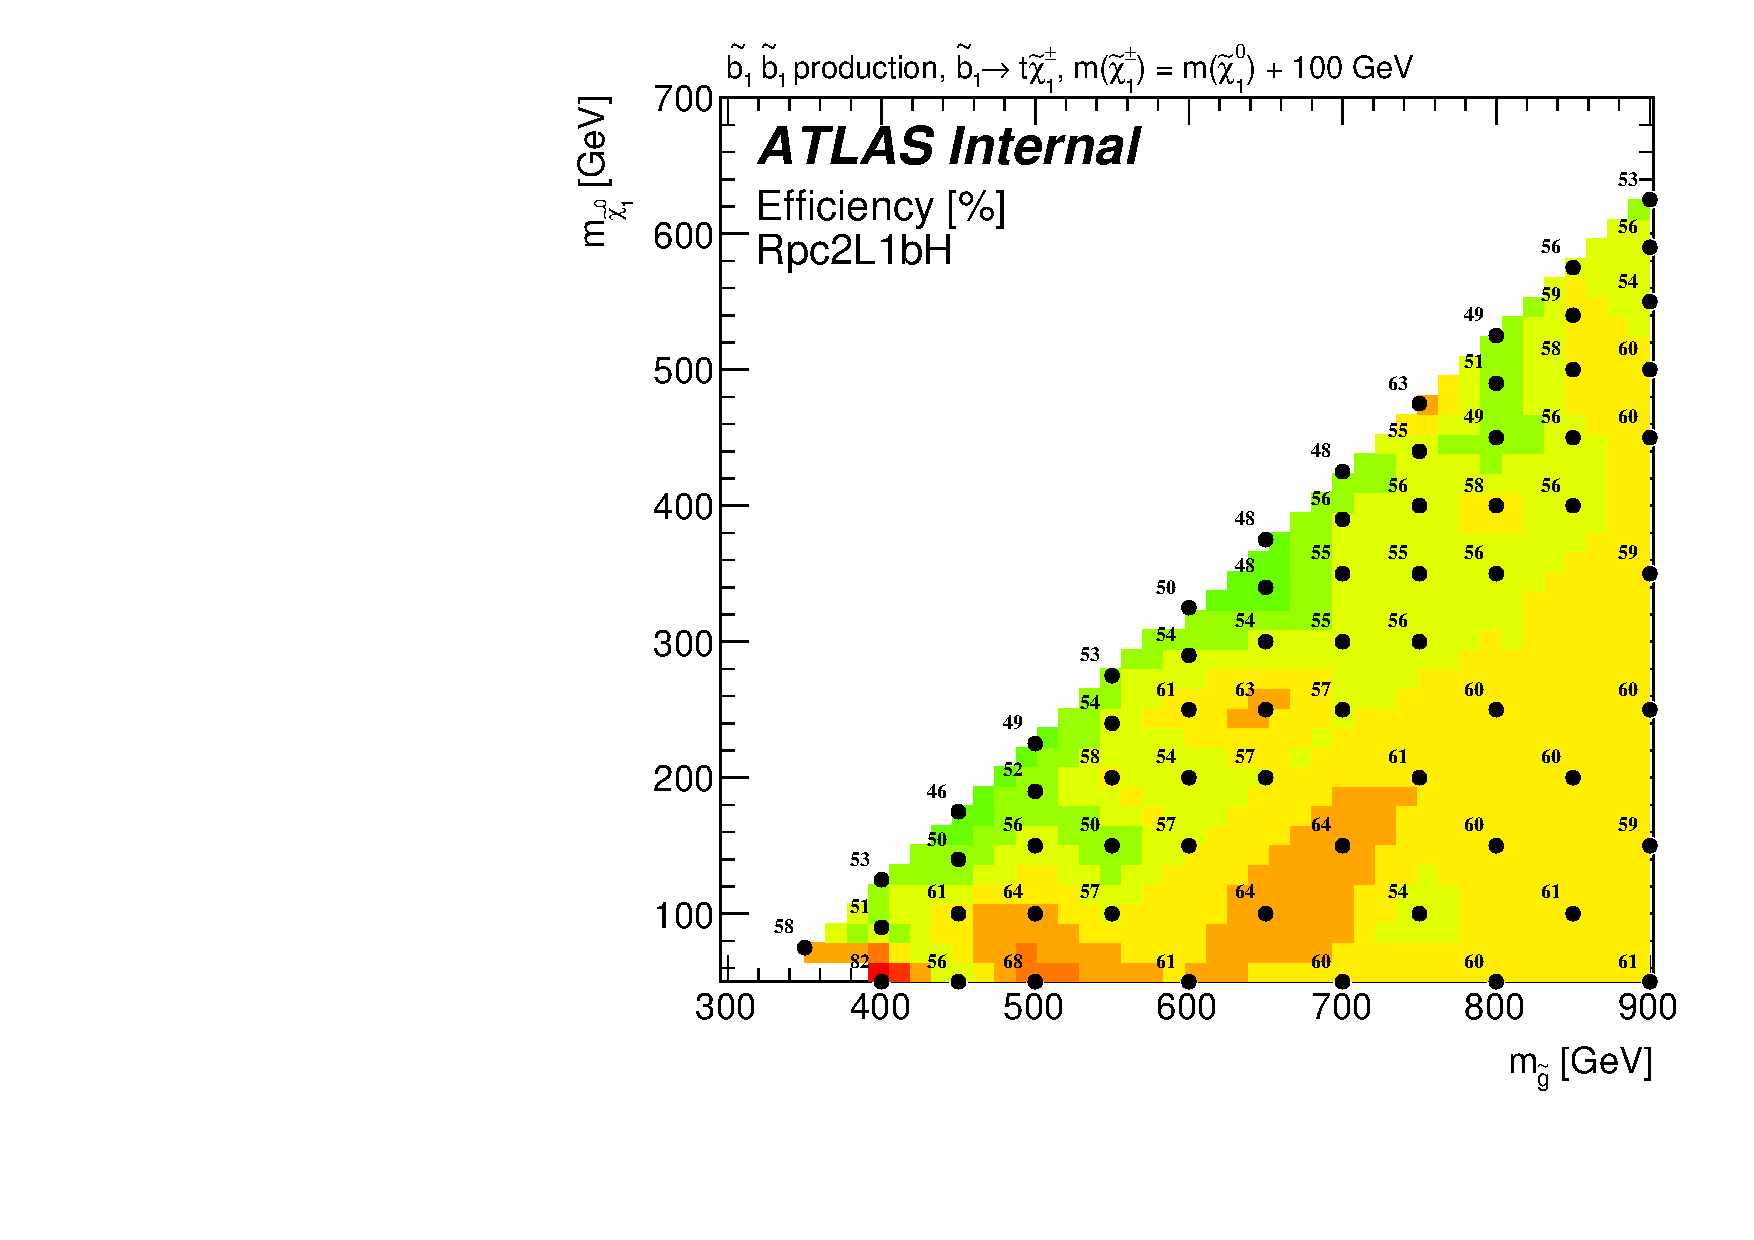
\includegraphics[width=\textwidth]{EffAcc/efficiency_BttRpc2L1bH}\caption{Rpc2L1bH efficiency}\end{subfigure}
\begin{subfigure}[t]{0.49\textwidth}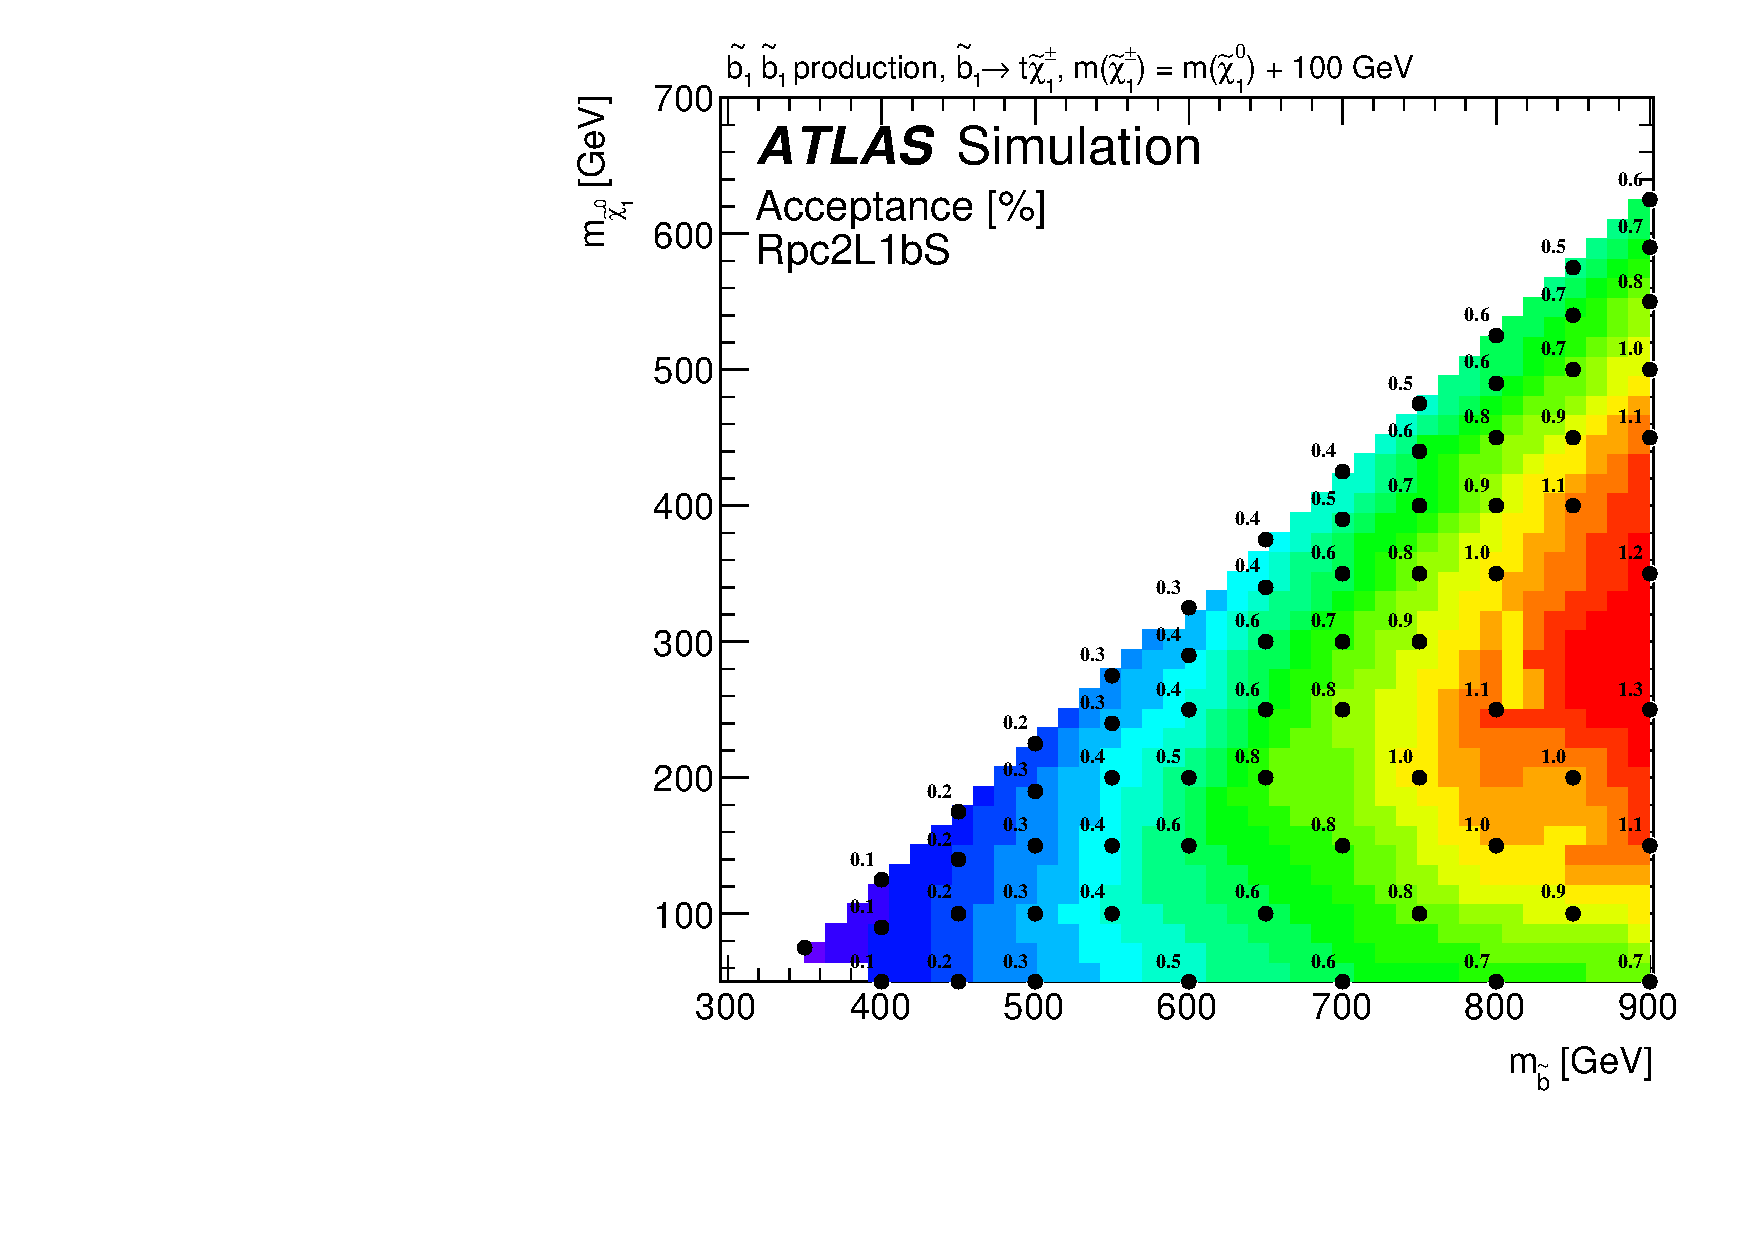
\includegraphics[width=\textwidth]{EffAcc/acceptance_BttRpc2L1bS}\caption{Rpc2L1bS acceptance}\end{subfigure}
\begin{subfigure}[t]{0.49\textwidth}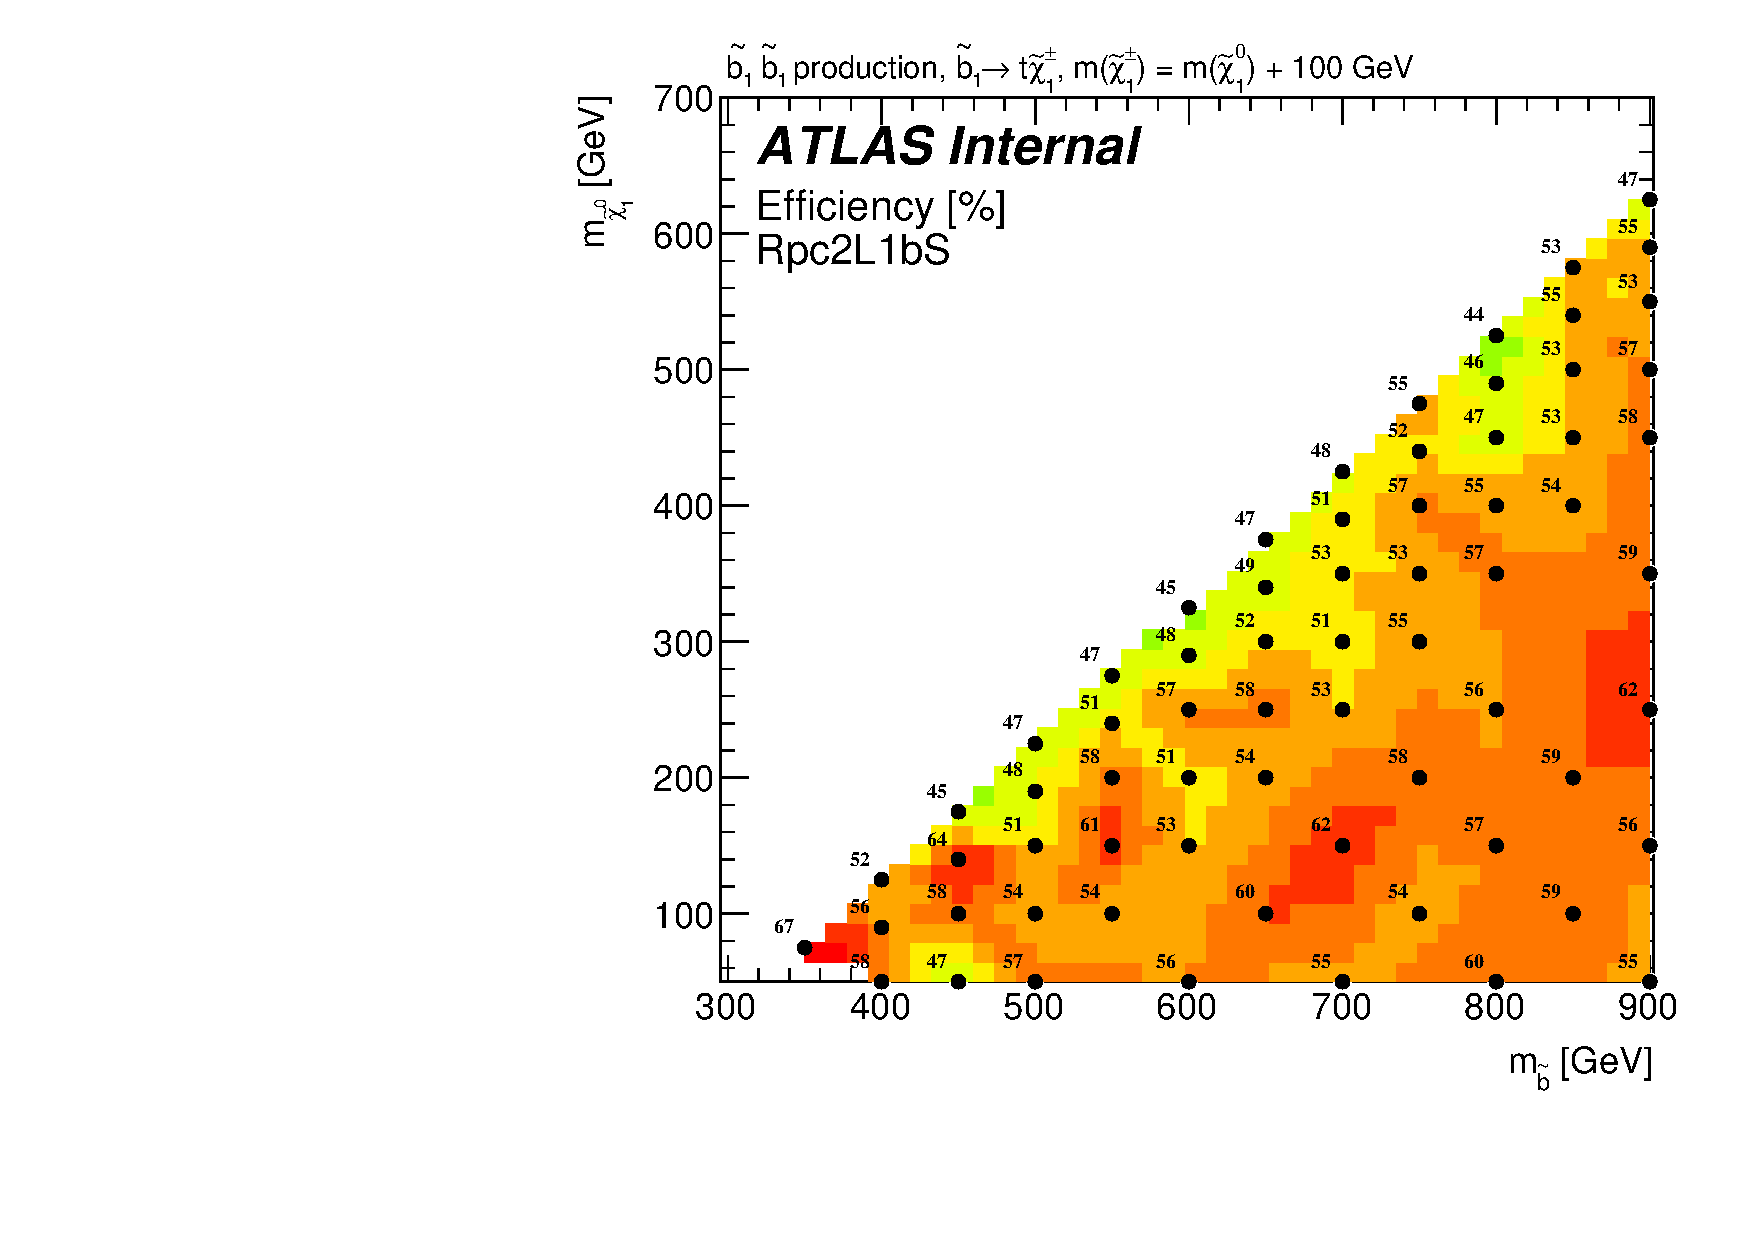
\includegraphics[width=\textwidth]{EffAcc/efficiency_BttRpc2L1bS}\caption{Rpc2L1bS efficiency}\end{subfigure}
\caption{Signal acceptance (a,c) and reconstruction efficiency (b,d) 
for simplified models of $\sbottomone\sbottomonebar$ production with $\sbottomone\to tW^{-}\ninoone$ decays, 
in the signal regions Rpc2L1bH (a,b) and Rpc2L1bS (c,d).}
\end{figure}


\begin{table}[htb!]\centering\begin{tabular}{|l|c|c|c|c|c|c|c|}\hline
\multicolumn{8}{|l|}{Rpc2L2bH,\quad $\gluino\gluino$ production in the NUHM2 model}\\\hline
$m_{\gluino}$ [GeV] & 300 & 350 & 400 & 500 & 600 & 700 & 800 \\\hline
Acceptance & 0.8\% & 1.6\% & 2.1\% & 3.2\% & 3.5\% & 4.4\% & 4.0\% \\
Efficiency & 43\% & 49\% & 50\% & 49\% & 48\% & 43\% & 49\%\\\hline
\end{tabular}
\caption{Rpc2L2bH signal region acceptance and reconstruction efficiency for $\gluino\gluino$ production in the NUHM2 model.}
\end{table}

\begin{table}[htb!]\centering\begin{tabular}{|l|c|c|c|c|c|c|}\hline
\multicolumn{7}{|l|}{Rpc3LSS1b,\quad $\stopone\stoponebar$ production,\quad $\stopone\to t\ninotwo$, $\ninotwo\to W^\mp\chargino$}\\\hline
$m_{\stopone}$ [GeV] & 550 & 600 & 650 & 700 & 750 & 800 \\\hline
Acceptance & 0.3\% & 0.3\% & 0.3\% & 0.4\% & 0.4\% & 0.4\%\\
Efficiency & 36\% & 42\% & 44\% & 37\% & 33\% & 30\%\\\hline
\end{tabular}
\caption{Rpc3LSS1b signal region acceptance and reconstruction efficiency for $\stopone\stoponebar$ production with $\stopone\to t\ninotwo$ ($\ninotwo\to W\chargino$) decays.}
\end{table}
